\documentclass[12pt,a4paper,twoside,openany]{book}
%\usepackage[work]{MCthesis}            % you can select this to work

\usepackage[final]{MCthesis}            % this is for the final submission

%%%%%%%%%%%%%%%%%%%%%%%%%%%%%%%%%%%%%%%%%%%%%%%%%%%%%%
%%%%%%%%%%%%%%%%%%%%%%%%%%%%%%%%%%%%%%%%%%%%%%%%%%%%%%
\usepackage[utf8]{inputenc}         % allow utf-8 input
% ------------------------------------------
\usepackage[T1]{fontenc}            % use 8-bit T1 fonts
\usepackage{hyperref}               % hyperlinks

% Hiding the red boxes around links
\hypersetup{
    hidelinks
}

\usepackage{url}                    % simple URL typesetting
\usepackage{booktabs}               % professional-quality tables
\usepackage{nicefrac}               % compact symbols for 1/2, etc.
\usepackage{microtype}              % microtypography
\usepackage{xcolor}                 % colors
\usepackage{amssymb,amsmath,amsfonts,amsbsy, amsthm}
\usepackage{mathrsfs}
\usepackage{bm}                     % bold vectors
\usepackage{listings}               % to include R-Code
\usepackage[section]{placeins}      % forces floats to appear in the section they are placed in
\usepackage[]{apacite}              % bibliography example
\usepackage[toc,page]{appendix}
\usepackage{framed}
\usepackage{float}
\usepackage{algorithm}              % For your pseudo-code
\usepackage{algpseudocode}          % For your pseudo-code
\usepackage[font=small, labelfont=bf, textfont=it]{caption}
%%%%%%%%%%%%%%%%%%%%%%%%%%%%%%%%%%%%%%%%%%%%%%%%%%%%%%
%%%%%%%%%%%%%%%%%%%%%%%%%%%%%%%%%%%%%%%%%%%%%%%%%%%%%%
\usepackage{blindtext}

%%%%%%%%%%%%%%%%%%%%%%%%%%%%%%%%%%%%%%%%%%%%%%%%%%%%
% SET VARIABLES FOR TITLE PAGE
\title{Optimal Transport in linear Independent Component Analysis}
\author{Ashutosh Jha}
\fromCity{Tuebingen}
\matnr{6639615}
\date{\today} % submission date

%%%%%%%%%%%%%%%%%%%%%%%%%%%%%%%%%%%%%%%%%%%%%%%%%%%%
%%%%%%%%%%%%%%%%%%%%%%%%%%%%%%%%%%%%%%%%%%%%%%%%%%%%
% SET VARIABLES FOR SUPERVISION AND EXAMINERS
\supervisor{Prof. Dr. Joachim Grammig\textsuperscript{1}}
           {Prof. Dr. Michel Besserve\textsuperscript{2,3}}
           {Dr. Simon Buchholz\textsuperscript{2}}

\reviewer{Prof. Dr. Joachim Grammig\textsuperscript{1}}
         {Prof. Dr. Augustin Kelava\textsuperscript{4}
          \\[1.5cm] % Adds space before the affiliations
          \multicolumn{2}{l}{\small \textsuperscript{1} Chair of Statistics, Econometrics and Empirical Economics, University of Tübingen} \\
          \multicolumn{2}{l}{\small \textsuperscript{2} Empirical Inference, Max Planck Institute for Intelligent Systems, Tübingen} \\
          \multicolumn{2}{l}{\small \textsuperscript{3} Institute for Machine Learning and AI, TU Braunschweig} \\
          \multicolumn{2}{l}{\small \textsuperscript{4} Methods Center, University of Tübingen}
         }
         {}
%%%%%%%%%%%%%%%%%%%%%%%%%%%%%%%%%%%%%%%%%%%%%%%%%%%%

%%%%%%%%%%%%%%%%%%%%%%%%%%%%%%%%%%%%%%%%%%%%%%%%%%%%%%%%%%%%%%%%%%%

% --- Better Float Parameters ---
\setcounter{topnumber}{2}
\setcounter{bottomnumber}{2}
\setcounter{totalnumber}{4}
\renewcommand{\topfraction}{0.85}
\renewcommand{\bottomfraction}{0.85}
\renewcommand{\textfraction}{0.15}
\renewcommand{\floatpagefraction}{0.8}
% -------------------------------

\begin{document}

% The \maketitle command in your MCthesis package automatically handles 
% the title page, declaration, \frontmatter, \tableofcontents, and \mainmatter.
\maketitle

\clearpage
\listoffigures
\clearpage
\listoftables
\cleardoublepage

% -----------------------------------------------------------------
% CHAPTER 1: INTRODUCTION
% -----------------------------------------------------------------
\chapter{Introduction}

\section{Motivation: Disentangling Latent Variables}
Blind Source Separation, specifically formulated as Independent Component Analysis (ICA), is a fundamental problem in modern statistics \cite{jutten1985}. 
It has widespread applications across diverse fields, including machine learning, signal processing, econometrics, and neuroscience. 
The primary objective of ICA is to recover hidden, statistically independent sources from an observed set of mixtures. 
In this thesis, we focus on the linear mixture setting. ICA is frequently contrasted with Principal Component Analysis (PCA); 
however, while PCA merely ensures that the resulting components are uncorrelated, ICA enforces the much stronger condition of full statistical independence \cite[Chapter 1]{hyvarinen2001}. 
This rigorous criterion allows ICA to successfully disentangle complex latent variables that PCA cannot fully separate.

\section{Intuition from Central Limit Theorem (CLT)}
For the linear ICA model to be identifiable, a strict condition must be met: at most one of the underlying independent sources can follow a Gaussian distribution. 
If multiple sources are Gaussian, any linear combination of them results in another Gaussian distribution, 
rendering the original signals rotationally symmetric and impossible to uniquely separate. 
This fundamental limitation naturally translates the challenge of finding independent components into an optimization problem: we must find the projections that maximize non-Gaussianity.

The theoretical justification for this approach is deeply rooted in the Central Limit Theorem (CLT). 
The CLT establishes that the sum or any linear combination of independent random variables tends toward a Gaussian distribution, 
regardless of the distributions of the original variables. Consequently, any observed mixture of independent, 
non-Gaussian sources will inherently appear more Gaussian than the constituent sources themselves. 
Therefore, by extracting the components that are the least Gaussian, we are effectively isolating the original independent signals.

\section{Information Theory, Thermodynamics and CLT}
The use of non-gaussianity as a measure for independence of components is also motivated by information 
theory. For a continuous random variable with a fixed variance, it is a foundational result that the Gaussian 
distribution uniquely possesses the maximum possible Shannon entropy. This mathematical property reveals a 
profound intrinsic link between information theory, the Central Limit Theorem, and statistical mechanics. 

In thermodynamics, isolated physical systems naturally evolve toward states of maximum entropy, or maximum 
disorder. Viewed through this interdisciplinary lens, the Central Limit Theorem serves as the statistical 
manifestation of this physical principle. The mathematical process of linearly mixing independent sources 
inherently increases the overall entropy of the system, inevitably driving the joint distribution toward 
the high-entropy Gaussian state. 

Recovering the underlying independent components, then, is conceptually equivalent to reversing this 
thermodynamic process. It requires projecting the empirical data away from the "disordered" high-entropy 
Gaussian manifold, intentionally guiding it back toward the highly structured, lower-entropy state of the 
original independent signals.

\section{Problem Statement and Research Objectives}
In practice, the ICA pipeline begins by centering and whitening the observed mixture. 
Whitening is a crucial preprocessing step that removes linear correlations and scales the variances to unity. Once the data is whitened, 
the search for independent components is geometrically restricted to finding an optimal orthogonal rotation. 
Specifically, the problem reduces to searching the unit sphere of the Stiefel manifold, space of orthogonal matrices, 
for the rotation matrix that maximizes the non-Gaussianity of the projected data.

The primary novelty of this research lies in proposing and investigating Optimal Transport metric, the Wasserstein distance, as the objective function for this rotational search. 
Our objective is to find the orthogonal candidates on the unit sphere that maximize the Wasserstein distance to a standard normal distribution. 
While traditional ICA algorithms often rely on sample approximations of population moments (such as kurtosis) or surrogate information-theoretic measures (such as negentropy approximations), 
the Wasserstein metric offers a distinct advantage: 
it evaluates the true global geometry of the empirical distribution using order statistics (sorted data), providing a highly robust, non-parametric measure of distance to Gaussianity. 

\section{Structure of the Thesis}
The remainder of this thesis is structured as follows. Chapter 2 establishes the theoretical foundations of linear ICA, information geometry, and Optimal Transport. 
Chapter 3 formalizes the Optimal Transport ICA (OT-ICA) framework, proving that the squared Wasserstein ($W_2^2$) distance rigorously bounds mixture non-Gaussianity. 
Chapter 4 details the algorithmic enhancements required to optimize this metric on the Stiefel manifold efficiently. 
Chapter 5 presents our experimental evaluation, demonstrating the failure modes of standard proxy optimization (such as FastICA) and proposing a robust ground cost modification to handle outliers. 
Finally, Chapter 6 concludes the thesis with a summary of findings and directions for future research.


% -----------------------------------------------------------------
% CHAPTER 2: THEORETICAL FOUNDATIONS
% -----------------------------------------------------------------
\chapter{Theoretical Foundations}

\section{Linear Independent Component Analysis (ICA)}

\subsection{Notation and the Linear Mixing Model}
The foundational assumption of the linear Independent Component Analysis model is that the observed signals are generated by a linear combination of statistically independent latent sources. 
Let the observed data be denoted by a random vector $\mathbf{X} \in \mathbb{R}^d$, and the latent independent sources by $\mathbf{S} \in \mathbb{R}^d$. 
The linear mixing model is formally defined as
\begin{equation}
    \mathbf{X} = \mathbf{A} \mathbf{S}
\end{equation}
where $\mathbf{A} \in \mathbb{R}^{d \times d}$ is an unknown, invertible mixing matrix \cite[Chapter7]{hyvarinen2001}. Expanded into vector notation, the model represents the observed variables as
\begin{equation}
    \begin{bmatrix}
    x_1 \\
    x_2 \\
    \vdots \\
    x_d
    \end{bmatrix}
    = 
    \begin{bmatrix}
    a_{11} & a_{12} & \cdots & a_{1d} \\
    a_{21} & a_{22} & \cdots & a_{2d} \\
    \vdots & \vdots & \ddots & \vdots \\
    a_{d1} & a_{d2} & \cdots & a_{dd}
    \end{bmatrix}
    \begin{bmatrix}
    s_1 \\
    s_2 \\
    \vdots \\
    s_d
    \end{bmatrix}.
\end{equation}
The core objective of ICA is to estimate an unmixing matrix $\mathbf{B} \approx \mathbf{A}^{-1}$ such that the recovered components $\mathbf{Z} = \mathbf{B}\mathbf{X}$ are as 
statistically independent as possible, thereby reconstructing the original sources $\mathbf{S}$.

\subsection{Identifiability and Ambiguities}
For the linear ICA model to be identifiable, it is a strict mathematical requirement that at most one of the underlying sources $s_i$ follows a Gaussian distribution. 
If two or more sources are Gaussian, any orthogonal transformation of those sources yields another set of independent Gaussian variables. Consequently, 
the mixing matrix cannot be uniquely determined from the observed data. Furthermore, even when the non Gaussianity assumption is met, the ICA model contains two inherent ambiguities. 
First, the variances (energies) of the independent components cannot be determined, which leads to a scaling ambiguity. Second, the order of the sources is arbitrary, 
leading to a permutation ambiguity. These ambiguities are generally acceptable in practice because the structural shape and independence of the source distributions are preserved.

\subsection{Centering and Whitening}
To simplify the optimization problem, the observed data $\mathbf{X}$ is subjected to a two step preprocessing phase consisting of centering and whitening. 
Centering ensures that the data has a zero mean by subtracting the expectation
\begin{equation}
    \mathbb{E}[\mathbf{X}] = \mathbf{0}.
\end{equation}
Given centered data, the covariance matrix simplifies to $\mathrm{Cov}(\mathbf{X}) = \mathbb{E}[\mathbf{X}\mathbf{X}^\top]$. 
Whitening is then applied to transform the observed vector into a new vector $\widetilde{\mathbf{X}}$ whose components are uncorrelated and possess unit variance. 
This is achieved using the eigenvalue decomposition of the covariance matrix
\begin{equation}
    \mathrm{Cov}(\mathbf{X}) = \mathbf{V}\mathbf{\Lambda}\mathbf{V}^\top
\end{equation}
where $\mathbf{V}$ is the orthogonal matrix of eigenvectors and $\mathbf{\Lambda}$ is the diagonal matrix of eigenvalues $\lambda_j$. 
The whitening transformation matrix $\mathbf{W}$ is constructed by scaling the eigenvectors by the inverse square root of the eigenvalues
\begin{equation}
    \mathbf{W} = \mathbf{\Lambda}^{-1/2} \mathbf{V}^\top.
\end{equation}
Applying this transformation yields the whitened data $\widetilde{\mathbf{X}} = \mathbf{W}\mathbf{X}$. The covariance of this new variable is the identity matrix
\begin{equation}
    \mathrm{Cov}(\widetilde{\mathbf{X}}) = \mathbf{W} \mathbb{E}[\mathbf{X}\mathbf{X}^\top] \mathbf{W}^\top = \mathbf{\Lambda}^{-1/2} \mathbf{V}^\top \mathbf{V} \mathbf{\Lambda} \mathbf{V}^\top \mathbf{V} \mathbf{\Lambda}^{-1/2} = \mathbf{I}_d.
\end{equation}
After whitening, the search for the unmixing matrix is drastically simplified. 
If we define the unmixing operation on the whitened data as $\widetilde{\mathbf{Z}} = \mathbf{U} \widetilde{\mathbf{X}}$, the covariance of the recovered components is
\begin{equation}
    \mathrm{Cov}(\widetilde{\mathbf{Z}}) = \mathbf{U} \mathrm{Cov}(\widetilde{\mathbf{X}}) \mathbf{U}^\top = \mathbf{U} \mathbf{I}_d \mathbf{U}^\top = \mathbf{U}\mathbf{U}^\top.
\end{equation}
Because the independent components must have unit variance, we require $\mathbf{U}\mathbf{U}^\top = \mathbf{I}_d$. This reveals that the unmixing matrix $\mathbf{U}$ must be perfectly orthogonal. 
The ICA problem is thus reduced to finding an optimal rotation on the Stiefel manifold.

\subsection{The Insufficiency of Principal Component Analysis}
Principal Component Analysis is frequently used to decorrelate data, which corresponds to finding the matrix $\mathbf{V}^\top$ in the eigenvalue decomposition. 
However, making a sample decorrelated and whitened is not sufficient for source separation when the data is non Gaussian. 
Once the data is whitened such that $\mathbb{E}[\mathbf{X}\mathbf{X}^\top] = \mathbf{I}_d$, any rotational orientation satisfies the PCA criteria. 
For multivariate Gaussian distributions, decorrelation directly implies independence, leaving nothing further for PCA to accomplish. For non Gaussian data, however, 
higher order dependencies remain. ICA must therefore traverse the space of orthogonal matrices to find local optima of contrast functions such as $f(\mathbf{u}) = \mathbb{E}[(\mathbf{u}^\top \mathbf{X})^4]$ on the unit sphere $S_n$. 
Gradient descent and other optimization techniques are required to pinpoint the exact rotation that maximizes non Gaussianity and achieves full statistical independence.

\section{An Information Geometry Perspective on ICA}

\subsection{Product and Gaussian Manifolds}
Information geometry provides a rigorous framework for quantifying the relationship between independence and non Gaussianity by analyzing probability distributions as points on geometric manifolds. 
Following the perspective introduced by Cardoso \citeyear{cardoso2022}, ICA can be understood as projecting the empirical distribution onto two distinct subspaces. The first is the Product manifold $\mathcal{P}$, 
which contains all distributions where the components are strictly independent. The second is the Gaussian manifold $\mathcal{G}$, which encompasses all multivariate Gaussian distributions with zero mean and a fixed covariance structure. 
Standard decorrelation merely ensures that the covariance is diagonal, but full ICA operates at the intersection of these manifolds to find a linear transform that projects the empirical data as closely as possible onto the Product manifold \cite{cardoso2022}.

\begin{figure}[tbp]
    \centering
    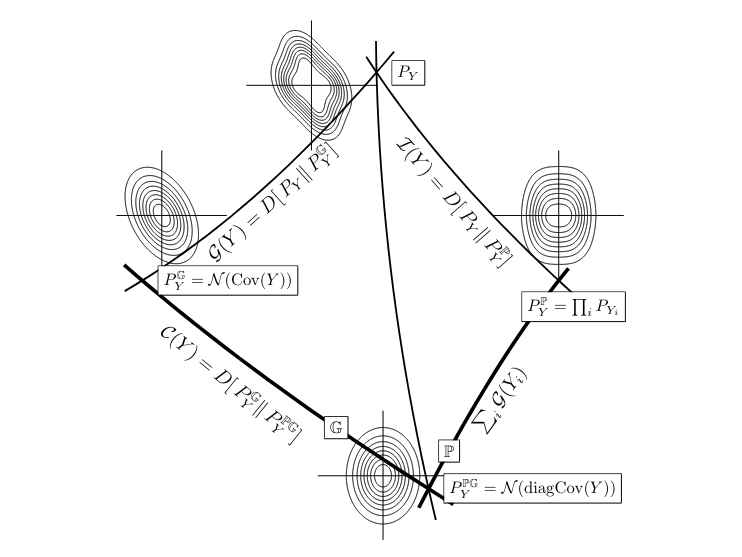
\includegraphics[width=0.85\textwidth]{pythagorean_ig_ica.png}
    \caption[Information Geometry of ICA]{The Pythagorean geometry of Independent Component Analysis. 
    The empirical joint distribution $P_Y$ is orthogonally projected onto the Product manifold $\mathcal{P}$ (yielding the independent marginals $P_Y^P$) 
    and the Gaussian manifold $\mathcal{G}$ (yielding the best Gaussian fit $P_Y^G$). The intersection of these approximations yields 
    the Product-Gaussian distribution $P_Y^{PG}$. The Kullback-Leibler divergences between these nodes geometrically represent distinct statistical properties: 
    Mutual Information $\mathscr{I}(Y) = D_{\mathrm{KL}}(P_Y \Vert P_Y^P)$, Joint Non-Gaussianity $G(Y) = D_{\mathrm{KL}}(P_Y \Vert P_Y^G)$, 
    and Correlation $C(Y) = D_{\mathrm{KL}}(P_Y^G \Vert P_Y^{PG})$. Figure adapted from \cite{cardoso2022}.}
    \label{fig:cardoso_geometry}
\end{figure}

\subsection{Kullback-Leibler Pythagorean Identities}
Distances between these distributions are measured using the Kullback-Leibler (KL) divergence. For any random vector $Y$ with a joint density $P_Y$, 
the mutual information $\mathscr{I}(Y)$ measures the distance to the closest independent product distribution
\begin{equation}
    \mathscr{I}(Y) = D_{\mathrm{KL}}\left(P_Y \,\Vert \, \prod_{i} P_{Y_i}\right).
\end{equation}
A Pythagorean identity exists on the Product manifold. For any candidate product distribution $Q = \prod_{i} q_i$, the divergence splits precisely into the mutual information and the marginal divergences
\begin{equation}
    D_{\mathrm{KL}}\left(P_Y \Vert Q\right) = \mathscr{I}(Y) + \sum_{i} D_{\mathrm{KL}}\left(P_{Y_i} \Vert q_i\right).
\end{equation}
A similar Pythagorean identity holds for the Gaussian manifold $\mathcal{G}$. The KL divergence from $P_Y$ to any arbitrary Gaussian distribution $\mathcal{N}(\Sigma)$ decomposes into 
the divergence to the best Gaussian fit and the divergence between the two Gaussian models
\begin{equation}
    D_{\mathrm{KL}}\big(P_Y \Vert \mathcal{N}(\Sigma)\big) = D_{\mathrm{KL}}\big(P_Y \Vert \mathcal{N}(\operatorname{Cov} Y)\big) + D_{\mathrm{KL}}\big(\mathcal{N}(\operatorname{Cov} Y) \Vert \mathcal{N}(\Sigma)\big).
\end{equation}

\subsection{Relating Independence, Correlation, and Non-Gaussianity}
These geometric identities can be combined to relate independence directly to non Gaussianity. We define the non Gaussianity of the joint variable $Y$ as $G(Y) = D_{\mathrm{KL}}(P_Y \,\Vert\, \mathcal{N}(\operatorname{Cov} Y))$, and the scalar measure of correlation as $C(Y) = D_{\mathrm{KL}}(\mathcal{N}(\operatorname{Cov} Y) \,\Vert\, \mathcal{N}(\operatorname{diag\,Cov} Y))$. Cardoso's unified theorem states that
\begin{equation}
    \mathscr{I}(Y) + \sum_{i} G(Y_i) = C(Y) + G(Y).
\end{equation}
Crucially, the joint non Gaussianity $G(Y)$ is invariant under invertible linear transformations. Furthermore, after the data has been whitened, 
the covariance matrix is the identity matrix, meaning $\operatorname{Cov}(Y) = \operatorname{diag\,Cov}(Y)$ and therefore the correlation term $C(Y) = 0$. 
The relationship then drastically simplifies to
\begin{equation}
    \mathscr{I}(Y) = G(Y) - \sum_{i} G(Y_i).
\end{equation}
Because $G(Y)$ is constant under rotation, minimizing the mutual information $\mathscr{I}(Y)$ is mathematically equivalent to maximizing the sum of the 
marginal non Gaussianities $\sum_i G(Y_i)$. This rigorously proves that centering and whitening constrain the data to a subspace where true statistical independence can be 
achieved solely by maximizing non Gaussianity \cite{cardoso2022}.

\section{Optimal Transport Theory}

\subsection{The Monge-Kantorovich Problem}
While information geometry utilizes Kullback-Leibler divergence, Optimal Transport offers an alternative metric space that is highly sensitive to the underlying geometry of the data. 
First formulated by Gaspard Monge \citeyear{monge1781}, the problem was originally conceptualized as finding the most cost effective way to move a distribution of mass, such as a pile of soil, 
to a target destination. 

Mathematically, this is framed as finding a transport map $T$ that pushes forward a source probability measure $\mu$ to a target measure $\nu$, denoted as $T_{\#} \mu = \nu$. 
This means that for any measurable set $A$, the mass assigned by $\nu$ is equal to the mass assigned by $\mu$ to the preimage of $A$, such that $\nu(A) = \mu(T^{-1}(A))$. 
Because finding a deterministic map $T$ is highly restrictive, Kantorovich \citeyear{kantorovich1942} later relaxed this formulation by introducing transport plans. This allowed mass from a single source 
location to be split and distributed across multiple targets. This relaxation transformed the rigorous mapping requirement into a joint probability distribution problem, 
making the computation of transport costs mathematically tractable.

\subsection{The Earth Mover's Distance ($W_1$)}
The minimal cost required to transform one probability distribution into another is formalized as the Wasserstein distance \cite[Chapter 1]{villani2003}. 
The $W_1$ distance, commonly referred to as the Earth Mover's Distance, 
quantifies the absolute effort of this transformation. For one dimensional distributions with cumulative distribution functions $F$ and $G$, the $W_1$ distance is computed as the integral of the 
absolute differences between the cumulative functions
\begin{equation}
    W_1(\mu, \nu) = \int_{-\infty}^\infty |F(x) - G(x)| \, dx.
\end{equation}
Intuitively, $W_1$ sums the vertical area between the two distribution curves. While this metric is robust to extreme outliers, it often underestimates structural deviations in variance.

\subsection{The Squared Wasserstein Distance ($W_2$)}
To better capture variations in spread and central location, the Squared Wasserstein distance is utilized \cite[Chapter 2]{villani2003}. It is most conveniently defined using the quantile functions, 
which are the inverses of the cumulative distribution functions $F^{-1}$ and $G^{-1}$. The $W_2$ distance is formulated as
\begin{equation}
    W_2(\mu, \nu) = \left( \int_0^1 |F^{-1}(t) - G^{-1}(t)|^2 \, dt \right)^{1/2}.
\end{equation}
By squaring the transport cost, the $W_2$ metric heavily penalizes local geometric distortions. When evaluating the distance between an empirical projection and a 
standard normal distribution $\mathcal{N}(0,1)$, $W_2$ provides a highly sensitive and reliable measure of Gaussianity. This makes it an ideal contrast function for Independent Component Analysis, 
as it maps the exact geometric deformations required to transform the candidate components into Gaussian noise.

\subsection{Brenier's Theorem and Caffarelli's Regularity}
\label{sec:brenier_caffarelli}
While the $W_1$ distance (often called the Earth Mover's Distance) offers an intuitive measure of transport, the transition to the squared Euclidean cost in 
the $W_2$ distance unlocks geometric properties that are essential for stable optimization. The analytical behavior of this distance is governed by 
two foundational pillars of optimal transport theory: Brenier's Theorem and Caffarelli's Regularity.

\paragraph{The Monge Map and Brenier's Theorem}
Brenier's Theorem essentially provides the proof of existence for a well-behaved functional relationship between our data and our target \cite{brenier1991}. 
It states that if our source distribution $\mu$ (our empirical data projection) is absolutely continuous, there exists a unique, deterministic way to push that data onto 
the target distribution $\nu$ (the Gaussian baseline). 

In the nomenclature of optimal transport, this unique assignment is called a \textit{Monge or Transport map}, denoted as $T$. Crucially, Brenier proved that this optimal map is not 
an arbitrary rearrangement; rather, it is the gradient of a convex potential function $\phi$, such that $T = \nabla \phi$. This is a powerful result for 
Independent Component Analysis (ICA) because it implies that the ``work'' required to transform our data into a Gaussian state follows a structured, mathematically conservative path, 
conceptually similar to an object moving through a gravitational potential field.

\paragraph{Smoothness and Caffarelli's Regularity}
While Brenier ensures that an optimal map exists, Caffarelli's regularity theory dictates how well-behaved that map is \cite{caffarelli1992}. In simple terms, 
Caffarelli demonstrated that if both our source and target probability densities are smooth and strictly bounded away from zero on their supports, 
the transport map $T$ will also be smooth and continuously differentiable. 

For the OT-ICA framework, this regularity is a vital mathematical safeguard. It guarantees that as we rotate our unmixing matrix on the Stiefel manifold (set of orthogonal matrices), 
the probability space is not being torn or folded abruptly. Instead, the transition from a non-Gaussian mixture to a Gaussian target occurs through a series of smooth, 
predictable deformations. This differentiability is precisely what allows us to reliably calculate gradients: if the transport map $T$ lacked this regularity, 
our optimization landscape would be littered with sharp discontinuities, making it nearly impossible for first-order solvers to find a stable global optimum.

% -----------------------------------------------------------------
% CHAPTER 3: THE OPTIMAL TRANSPORT ICA (OT-ICA) FRAMEWORK
% -----------------------------------------------------------------
\chapter{The Optimal Transport ICA (OT-ICA) Framework}

\section{Formulating ICA as an Optimal Transport Problem}
As established in the preceding chapter, the process of centering and whitening restricts the search for independent 
components to the manifold of orthogonal matrices. Furthermore, Cardoso's unified theorem \cite{cardoso2022} demonstrates 
that within this whitened space, the mutual information of the projections is minimized precisely when the sum of their 
marginal non-Gaussianities is maximized. Traditional Independent Component Analysis algorithms approach this optimization 
by utilizing proxy contrast functions, such as kurtosis or negentropy approximations. While computationally inexpensive, 
these proxies often capture only specific statistical moments, ignoring the broader geometric structure of the underlying probability distributions.

This thesis proposes a paradigm shift by formulating ICA directly as an Optimal Transport problem. Instead of relying on 
proxy moments, we utilize the squared Wasserstein distance, $W_2^2$, as a direct, geometrically rigorous measure of non-Gaussianity. 
Let $\mathbf{X}$ be the whitened observed mixture, and let $\mathbf{u} \in S_n$ be a candidate projection vector on the unit sphere. 
The empirical distribution of the projected data is denoted by $\mathbb{P}_{\mathbf{u}^\top \mathbf{X}}$. We formally define the 
objective of the OT-ICA framework as finding the orthogonal rotation matrix whose column vectors $\mathbf{u}$ maximize the 
transport cost to a standard normal distribution $\mathcal{N}(0,1)$:
\begin{equation}
    \hat{\mathbf{u}} = \arg\max_{\mathbf{u} \in S_n} W_2^2\big(\mathbb{P}_{\mathbf{u}^\top \mathbf{X}}, \mathcal{N}(0,1)\big).
\end{equation}
By framing the problem in this manner, we leverage the Optimal Transport metric's unique ability to capture global geometric 
deviations from Gaussianity, providing a highly sensitive contrast function.

\section{Theoretical Motivation: Bounding Mixture Non-Gaussianity}
To mathematically justify the use of $W_2^2$ as an objective function for ICA, we must prove that maximizing this distance 
recovers the true independent sources. By the Central Limit Theorem, we possess the intuitive understanding that a mixture of 
non-Gaussian sources is more Gaussian than the constituent sources themselves. In the language of Optimal Transport, this implies 
that the Wasserstein distance between a mixture and a Gaussian distribution must be strictly bounded by the distances of its independent components. 


\subsection{Constructing the Common Source Coupling}
To formally prove this bound, we construct a specific joint probability distribution, or coupling, using a common source of randomness. 
Let $\mathbf{N} = (N_1, \dots, N_d)^\top$ be a vector of $d$ independent standard normal variables, such that $\mathbf{N} \sim \mathcal{N}(0, \mathbf{I}_d)$. 
For each true independent latent source $Z_i$, there exists an Optimal Transport map $T_i$ that pushes forward the standard normal distribution 
to the source distribution, denoted as $(T_i)_{\#} \mathcal{N}(0,1) = Z_i$. 

We can construct a random variable $X$ representing a linear mixture of the sources using a weight vector $\mathbf{w}$ defined on the 
unit sphere ($\sum_{i=1}^d w_i^2 = 1$). By applying the transport maps to our common noise vector, the mixture is defined as
\begin{equation}
    X = \sum_{i=1}^d w_i T_i(N_i).
\end{equation}
Because $T_i(N_i)$ follows the distribution of $Z_i$, it follows that $X$ perfectly models the weighted mixture $\mathbf{w} \cdot \mathbf{Z}$. 
To compare this mixture to a Gaussian distribution, we construct a target variable $Y$ using the exact same underlying noise vector $\mathbf{N}$ and the same weights:
\begin{equation}
    Y = \sum_{i=1}^d w_i N_i.
\end{equation}
Given that the weights sum to unity and the components $N_i$ are independent standard normals, the resulting variable $Y$ is guaranteed to follow 
a standard normal distribution, $Y \sim \mathcal{N}(0,1)$. The pair $(X, Y)$ therefore creates a valid coupling $\pi_{X,Y}^{\mathbf{N}}$ 
between the mixture distribution and the Gaussian target.

\subsection{Proof of the $W_2$ Upper Bound}
The squared Wasserstein distance is defined as the infimum of the expected squared cost over all possible valid couplings. 
Because the infimum represents the absolute optimal transport plan, the cost of the optimal plan must be less than or equal to the cost of our 
specifically constructed coupling $(X, Y)$. This yields the fundamental inequality:
\begin{equation}
    W_2^2(\mathbf{w} \cdot \mathbf{Z}, \mathcal{N}(0,1)) \le \mathbb{E}\left[|X - Y|^2\right].
\end{equation}
We evaluate the right side of this inequality by expanding the squared difference:
\begin{align}
    |X - Y|^2 &= \left| \sum_{i=1}^d w_i T_i(N_i) - \sum_{i=1}^d w_i N_i \right|^2 \nonumber \\
              &= \left( \sum_{i=1}^d w_i \big(T_i(N_i) - N_i\big) \right)^2.
\end{align}
Squaring the summation produces a combination of diagonal terms where $i=j$ and cross terms where $i \neq j$:
\begin{equation}
    |X - Y|^2 = \sum_{i=1}^d w_i^2 \big(T_i(N_i) - N_i\big)^2 + \sum_{i \neq j} w_i w_j \big(T_i(N_i) - N_i\big)\big(T_j(N_j) - N_j\big).
\end{equation}
Taking the mathematical expectation of this expansion drastically simplifies the expression. Because the underlying noise variables $N_i$ and $N_j$ are independent, 
and the functions evaluate to a mean of zero, the expectation of all cross terms strictly vanishes. We are left solely with the expectation of the diagonal terms:
\begin{equation}
    \mathbb{E}\left[|X - Y|^2\right] = \sum_{i=1}^d w_i^2 \mathbb{E}\left[ \big(T_i(N_i) - N_i\big)^2 \right].
\end{equation}
Recognizing that $\mathbb{E}[ (T_i(N_i) - N_i)^2 ]$ is the exact definition of the squared Wasserstein distance between the individual source $Z_i$ and a 
standard normal distribution, we arrive at the final upper bound:
\begin{equation}
    W_2^2(\mathbf{w} \cdot \mathbf{Z}, \mathcal{N}(0,1)) \le \sum_{i=1}^d w_i^2 W_2^2(Z_i, \mathcal{N}(0,1)).
\end{equation}
This convexity adjacent property proves that mixing independent sources mathematically reduces the Wasserstein distance to Gaussianity. 
Maximizing the left-hand side forces the weight vector $\mathbf{w}$ to collapse toward a canonical axis, effectively isolating a single independent source.

\subsection{Comonotonicity and the Proof of Strict Inequality}
While the upper bound demonstrates that mixtures do not exceed the non-Gaussianity of their sources, successfully optimizing ICA requires proving 
that mixtures are strictly less non-Gaussian than the original sources. We must therefore determine the conditions under which the aforementioned 
inequality becomes a strict inequality. 

In a one-dimensional setting, the $W_2$ distance equals the expected squared difference of a specific coupling if and only if the random variables 
are comonotonic. By Brenier's Theorem \cite{brenier1991}, this implies there exists a strictly increasing, deterministic function mapping one variable to the other. 
For our constructed mixture variable $X$ and the Gaussian target $Y$ to be comonotonic with respect to the shared noise vector $\mathbf{N} \in \mathbb{R}^d$, 
their gradients must be perfectly parallel at every point in the probability space. This requires the existence of a scalar scaling function $\lambda(\mathbf{N})$ such that:
\begin{equation}
    \nabla X(\mathbf{N}) = \lambda(\mathbf{N}) \nabla Y(\mathbf{N}).
\end{equation}

Assuming the source distributions possess smooth and strictly positive densities, Caffarelli's regularity theory \cite{caffarelli1992} guarantees that the 
Optimal Transport maps $T_i$ are continuously differentiable. We can therefore compute the gradients of our constructed variables with respect to the noise vector $\mathbf{N}$. 
The gradient of the Gaussian target is simply the weight vector:
\begin{equation}
    Y(\mathbf{N}) = \sum_{i=1}^d w_i N_i \implies \nabla Y = \mathbf{w}.
\end{equation}
The gradient of the source mixture leverages the derivatives of the individual transport maps:
\begin{equation}
    X(\mathbf{N}) = \sum_{i=1}^d w_i T_i(N_i) \implies \nabla X = \begin{bmatrix} w_1 T'_1(N_1) \\ w_2 T'_2(N_2) \\ \vdots \\ w_d T'_d(N_d) \end{bmatrix}.
\end{equation}

Substituting these gradients back into our comonotonicity condition yields the system of equations:
\begin{equation}
    \nabla X = \lambda(\mathbf{N}) \mathbf{w}.
\end{equation}
To determine if this condition can hold for non-Gaussian sources, we differentiate both the Left-Hand Side (LHS) and the Right-Hand Side (RHS) 
with respect to $\mathbf{N}$ to compute their respective Hessian (Jacobian) matrices.

On the left hand side, because $X$ separates into independent terms $w_i T_i(N_i)$, the cross-derivatives $\frac{\partial^2 X}{\partial N_i \partial N_j}$ 
are strictly zero for all $i \neq j$. This yields a purely diagonal matrix containing the second derivatives of the transport maps.

On the right hand side,we differentiate the product $\lambda(\mathbf{N}) \mathbf{w}$. Because the weight vector $\mathbf{w}$ is a constant, 
applying the product rule yields the outer product of $\mathbf{w}$ and the gradient of the scalar function $\nabla \lambda$. This forms a Rank-1 matrix.

Equating the left and right hand sides:
\begin{equation}
    \underbrace{
    \begin{bmatrix} 
    w_1 T''_1(N_1) & 0 & \cdots & 0 \\
    0 & w_2 T''_2(N_2) & \cdots & 0 \\
    \vdots & \vdots & \ddots & \vdots \\
    0 & 0 & \cdots & w_d T''_d(N_d)
    \end{bmatrix}
    }_{\text{Hessian of } X \text{ (Diagonal)}}
    =
    \underbrace{
    \begin{bmatrix}
    w_1 \frac{\partial \lambda}{\partial N_1} & w_1 \frac{\partial \lambda}{\partial N_2} & \cdots & w_1 \frac{\partial \lambda}{\partial N_d} \\
    w_2 \frac{\partial \lambda}{\partial N_1} & w_2 \frac{\partial \lambda}{\partial N_2} & \cdots & w_2 \frac{\partial \lambda}{\partial N_d} \\
    \vdots & \vdots & \ddots & \vdots \\
    w_d \frac{\partial \lambda}{\partial N_1} & w_d \frac{\partial \lambda}{\partial N_2} & \cdots & w_d \frac{\partial \lambda}{\partial N_d}
    \end{bmatrix}
    }_{\text{Outer Product } \mathbf{w} (\nabla \lambda)^\top \text{ (Rank-1)}}
\end{equation}

This matrix equality forces a profound contradiction. Let us examine any off-diagonal entry located at row $i$ and column $j$ (where $i \neq j$). 
The diagonal LHS matrix dictates that this entry must be exactly zero. However, the RHS Rank-1 matrix evaluates this same entry as $w_i \frac{\partial \lambda}{\partial N_j}$. 
This establishes the requirement:
\begin{equation}
    w_i \frac{\partial \lambda}{\partial N_j} = 0 \quad \text{for all } i \neq j.
\end{equation}
Because we are assuming a valid mixture where the component weights are non-zero ($w_i \neq 0$), it must be true that $\frac{\partial \lambda}{\partial N_j} = 0$. 
Since this holds across all dimensions, the gradient of the scaling function is zero ($\nabla \lambda = \mathbf{0}$). 
Consequently, $\lambda(\mathbf{N})$ must be a global scalar constant, $\lambda$.

If $\lambda$ is a constant, then equating the diagonal elements of our matrices implies that $T'_i(N_i) = \lambda$. Integrating this relationship means the 
Optimal Transport maps themselves must be strictly linear functions of the form:
\begin{equation}
    T_i(x) = \lambda x + c.
\end{equation}
We know that applying a purely linear transformation to a Gaussian noise source $N_i$ can only ever produce another Gaussian distribution. 
However, the foundational identifiability assumption of ICA guarantees that our original latent sources $Z_i$ are non-Gaussian. Because the sources are non-Gaussian, 
their Optimal Transport mappings from a Gaussian base must be non-linear (curved). 

Therefore, the linear map requirement derived from the comonotonicity condition fundamentally fails for non-Gaussian sources. 
Because the condition for equality cannot be met, we conclude that for any valid mixture of independent, non-Gaussian variables, the relationship is a strict inequality:
\begin{equation}
    W_2^2(\mathbf{w} \cdot \mathbf{Z}, \mathcal{N}(0,1)) < \sum_{i=1}^d w_i^2 W_2^2(Z_i, \mathcal{N}(0,1)).
\end{equation}

\section{Empirical Landscape: $W_1$ versus $W_2^2$}
Having established the theoretical foundations of the $W_2^2$ metric, specifically the existence of a smooth, conservative transport map via Brenier and Caffarelli (Section \ref{sec:brenier_caffarelli}), 
we must evaluate its practical suitability for manifold optimization. In the context of ICA, the objective is to \textit{maximize} non-Gaussianity. 
Therefore, gradient ascent algorithms must climb the loss landscape to locate the peaks (maxima) of the distance metric to successfully isolate the independent sources.

While the $W_1$ distance (Earth Mover's Distance) is highly robust to outliers, its reliance on an $L_1$ absolute penalty introduces severe geometric pathologies 
when applied to finite empirical samples. We demonstrate why the squared $L_2$ penalty of the $W_2^2$ metric is better for gradient-based convergence.

\subsection{Empirical Gradients and Derivative Volatility}
To conduct this empirical comparison, we generated a synthetic bivariate mixture of Student-t distributions ($\nu=4$) and systematically evaluated 
both the raw distances and their first-order numerical gradients across a continuous sweep of rotation angles $\theta \in [0, \pi]$. 
Because the unmixing matrix restricts the search to orthogonal vectors, the two true independent components are geometrically separated by exactly $\pi/2$ radians ($90^\circ$).

\begin{figure}[tbp]
    \centering
    
\includegraphics[width=1.0\textwidth]{w1_vs_w2_derivatives.png} 
    \caption[Gradient Landscapes of $W_1$ and $W_2^2$]{The empirical optimization landscapes (top) and their normalized first derivatives (bottom). 
    While both metrics peak near the true independent components ($\theta \approx 0, \pi/2, \pi$), their gradient behaviors are fundamentally opposed. 
    The $W_2^2$ gradient smoothly decelerates to zero, whereas the $W_1$ gradient is highly volatile and jagged, demonstrating severe instability on finite samples.}
    \label{fig:w1_vs_w2_derivatives}
\end{figure}

The empirical results, visualized in Figure \ref{fig:w1_vs_w2_derivatives}, reveal a fundamental mathematical incompatibility between 
the $W_1$ metric and continuous gradient ascent. In Optimal Transport, because the $W_1$ cost scales strictly linearly with distance, 
the resulting optimization landscape lacks the strict convexity required to smooth out finite sample noise.

The consequence of this lack of curvature is very bad for numerical solvers, as clearly illustrated in the bottom gradient profile. 
Because $W_1$ relies on piecewise linear sorting mechanics without a squaring penalty to dampen local permutations, its empirical derivative is extremely noisy and volatile. 
It thrashes wildly as the projection angle rotates. Consequently, any first-order gradient ascent solver will suffer from uneven derivative surface, 
perpetually bouncing across local noise spikes without ever cleanly converging on the true peak. 
Furthermore, this high volatility renders second-order Quasi-Newton approximations (such as L-BFGS) completely useless, 
as no stable Hessian can be approximated from such a shattered gradient.

In contrast, the squared penalty of the $W_2^2$ metric acts as a natural mathematical smoother by heavily penalizing local geometric distortions. 
As illustrated in the gradient profiles, the $W_2^2$ derivative behaves as a stable, continuous sinusoidal wave that decelerates predictably as it approaches the global optimum. 
This retention of curvature provides a more reliable signal for gradient-based solvers, allowing the OT-ICA framework to converge more consistently 
than would be possible under the sharper, piecewise-linear landscape of the $W_1$ metric.


% -----------------------------------------------------------------
% CHAPTER 4: ALGORITHMIC DESIGN AND OPTIMIZATION
% -----------------------------------------------------------------
\chapter{Algorithmic Enhancements}

\section{The Baseline OT-ICA Algorithm}
Having established the theoretical optimality of the squared Wasserstein distance ($W_2^2$) for Independent Component Analysis, 
the challenge transitions to computationally minimizing this cost function. The baseline OT-ICA algorithm proceeds by first centering and whitening 
the observed mixture $\mathbf{X} \in \mathbb{R}^{d \times N}$, yielding the whitened data $\widetilde{\mathbf{X}}$. The algorithm then initializes 
an orthogonal unmixing matrix $\mathbf{W} \in \mathbb{R}^{d \times d}$. In the forward pass, the data is projected onto the candidate components, 
$\mathbf{Y} = \mathbf{W}\widetilde{\mathbf{X}}$. For each row (component) of $\mathbf{Y}$, the empirical cumulative distribution function is 
constructed by sorting the $N$ observations. The $W_2^2$ distance is then computed by matching these sorted empirical quantiles to the corresponding quantiles of a standard normal distribution. 

While theoretically sound, the naive implementation of this gradient descent loop faces severe computational and geometric hurdles. 
The exact Optimal Transport matching requires sorting at every iteration, presenting a significant computational bottleneck. 
Furthermore, standard gradient updates do not inherently respect the strict orthogonality constraint of the mixing matrix, 
and discrete approximations of the target Gaussian introduce gradient noise. To make OT-ICA computationally competitive with existing methods, 
several specific algorithmic and geometric enhancements are required.

\section{Computational Bottlenecks and Solutions}

\subsection{Exact Analytical Gaussian Targets}
A primary source of instability in the baseline algorithm is the discrete approximation of the target Gaussian distribution. 
Traditionally, the target quantiles are approximated by evaluating the inverse cumulative distribution function at evenly spaced intervals, 
such as $q_i = \Phi^{-1}((i - 0.5)/N)$. However, representing a continuous, infinite-tailed Gaussian distribution with a finite set of discrete points 
introduces approximation noise. When the algorithm computes the gradient of the $W_2^2$ distance, this noise translates into a jagged optimization landscape, 
severely hindering convergence as the components approach true independence.

To eliminate this approximation noise, we replace the point-sampled targets with an exact analytical formulation. Using integral calculus, 
we compute the exact expected value of a standard normal variable within each discrete quantile bin. Let the uniform probability bin edges be defined 
as $p_i = \frac{i}{N}$ for $i = 0, \dots, N$, with corresponding Gaussian domain boundaries $z_i = \Phi^{-1}(p_i)$. 
The exact analytical target value $T_i$ for the $i$-th sorted sample is computed as the conditional expectation within that interval:
\begin{equation}
    T_i = N \int_{z_{i-1}}^{z_i} x \phi(x) \, dx
\end{equation}
where $\phi(x)$ is the standard normal probability density function. Evaluating this integral yields the closed-form solution:
\begin{equation}
    T_i = N \big( \phi(z_{i-1}) - \phi(z_i) \big).
\end{equation}
By computing this exact analytical target once during initialization, the algorithm evaluates the $W_2^2$ distance against a mathematically perfect 
discrete representation of a Gaussian, ensuring perfectly smooth gradients near the global optimum.

\subsection{Batched Vectorization for Restarts}
Unlike Principal Component Analysis, which yields a unique global solution via singular value decomposition, 
the ICA optimization landscape is highly non-convex and characterized by numerous local optima. Consequently, 
identifying the true independent components strictly requires multiple random initializations (restarts) to thoroughly explore the hypothesis space. 

Because evaluating the $W_2^2$ objective inherently requires an $\mathcal{O}(N \log N)$ sorting operation for each candidate component, 
executing these random restarts sequentially via standard iterative loops is computationally prohibitive. To resolve this, we utilize a batched vectorization strategy. 
Rather than maintaining a single weight matrix, we aggregate $B$ random restarts into a single high-dimensional tensor $\mathbf{W}_{\text{batch}} \in \mathbb{R}^{B \times d \times d}$. 

This formulation allows the projection $\mathbf{Y} = \mathbf{W}_{\text{batch}} \widetilde{\mathbf{X}}$ to be computed simultaneously for all $B$ trajectories. 
The elements of the resulting batch tensor can be sorted in parallel. 
The pre-computed exact analytical target vector $\mathbf{T}$ is subsequently broadcast-subtracted across the entire batch to compute the distances and gradients in a single step.

\section{Optimization on the Stiefel Manifold}

\subsection{The Riemannian Gradient}
Because the input data is whitened, the unmixing matrix $\mathbf{W}$ must remain strictly orthogonal, satisfying $\mathbf{W}\mathbf{W}^\top = \mathbf{I}$. 
The geometric space of all such orthogonal matrices forms the Stiefel manifold, denoted $\mathcal{S}$. If we compute the standard Euclidean gradient of the squared Wasserstein distance, 
$\mathbf{G} = \nabla_{\mathbf{W}} W_2^2$, this vector points into the flat, unconstrained ambient space $\mathbb{R}^{d \times d}$. 
Updating the matrix using this Euclidean gradient would immediately violate the orthogonality constraint.

To navigate the curved geometry of the Stiefel manifold, we must project the Euclidean gradient onto the tangent space of the manifold at the current point $\mathbf{W}$, 
as illustrated in Figure \ref{fig:stiefel_manifold}. 

\begin{figure}[tbp]
    \centering
    
\includegraphics[width=0.75\textwidth]{stiefel_manifold_projection.png}
    \caption[Riemannian Optimization on the Stiefel Manifold]{Geometric sketch of optimization on the Stiefel manifold $\mathcal{S}$. 
    The Euclidean gradient $\mathbf{G}$ is projected onto the tangent space $T_{\mathbf{W}}\mathcal{S}$ to yield the Riemannian gradient $\nabla_{\mathcal{S}} \mathbf{W}$. 
    Following a step along the tangent plane, 
    a retraction maps the estimate back to the orthogonal manifold surface at $\mathbf{W}_{\text{new}}$.}
    \label{fig:stiefel_manifold}
\end{figure}

The resulting Riemannian gradient $\nabla_{\mathcal{S}} \mathbf{W}$ is given by \cite[Chapter 3]{absil2008optimization}:
\begin{equation}
    \nabla_{\mathcal{S}} \mathbf{W} = \mathbf{G} - \frac{1}{2}\big(\mathbf{G}\mathbf{W}^\top + \mathbf{W}\mathbf{G}^\top \big)\mathbf{W}.
\end{equation}
Geometrically, the term $(\mathbf{G}\mathbf{W}^\top + \mathbf{W}\mathbf{G}^\top)$ precisely measures the symmetric violation of orthogonality induced by the Euclidean gradient. 
By subtracting this specific violation, we ensure that the update step perfectly hugs the curvature of the manifold, preserving the decorrelation of the components.

\subsection{Retraction via Symmetric Decorrelation}
Although the Riemannian gradient ensures the update step is tangential to the Stiefel manifold, 
moving along this flat tangent plane for a finite step size $\eta$ will cause the new matrix $\mathbf{W}_{\text{step}} = \mathbf{W} - \eta \nabla_{\mathcal{S}} \mathbf{W}$ 
to slightly lift off the curved manifold surface. To restore exact orthogonality, the matrix must be mapped back onto the manifold 
via a mathematical operation known as a retraction \cite[Chapter 4]{absil2008optimization}.

While the Gram-Schmidt orthogonalization process is a common approach, it is fundamentally asymmetric; 
it permanently fixes the first vector and modifies subsequent vectors to fit, which inherently biases simultaneous optimization. 
Instead, we utilize symmetric decorrelation as our retraction mechanism:
\begin{equation}
    \mathbf{W}_{\text{new}} = (\mathbf{W}_{\text{step}}\mathbf{W}_{\text{step}}^\top)^{-1/2} \mathbf{W}_{\text{step}}.
\end{equation}
This operation computes the overlap covariance of the stepped matrix and applies a uniform, symmetric adjustment to all vectors simultaneously. 
This ensures that no single independent component is arbitrarily prioritized during the retraction process, maintaining the stability of the batched optimization.

\section{Total Complexity and Statistical Efficiency}
Having detailed the sorting-based objective and the Riemannian optimization steps, we can now formalize the total computational cost of the OT-ICA framework. 
For a dataset of dimension $d$ with $N$ samples, $K$ random restarts, and $T$ optimization iterations, the per-iteration complexity is dominated by:
\begin{equation}
    \mathcal{O}(K \cdot (d \cdot N \log N + d^3))
\end{equation}
The $N \log N$ term stems from the mandatory sorting of projections, while the $d^3$ term represents the cost of the symmetric decorrelation (matrix inverse square root) 
used for retraction on the Stiefel manifold.

Beyond temporal complexity, we must acknowledge the \textit{statistical sample complexity}. While our 1D projection approach maintains a robust 1D convergence rate 
of $\mathcal{O}(N^{-1/2})$, the global identification of the mixing matrix is implicitly subject to the curse of dimensionality. Theoretical results in transport theory suggest 
that the empirical Wasserstein distance in $d$ dimensions converges at a rate of $\mathcal{O}(N^{-1/d})$. In practice, as $d$ increases, the number of samples $N$ required to 
accurately resolve the 'peaks' of non-Gaussianity on the manifold surface grows. This necessitates a corresponding increase in the number of parallel restarts $K$, creating 
a trade-off between statistical resolution and computational feasibility.

\section{Navigating Discrete Optimization Landscapes}
While the OT-ICA framework demonstrates robust convergence on continuous distributions, real-world data often contains discrete signals, such as binary states, 
digital communications, or count-based market events. Applying continuous Optimal Transport directly to discrete mixtures introduces severe geometric pathologies 
that fracture the optimization landscape.

\subsection{The Shattered Landscape of Discrete CDFs}
The exact analytical Gaussian target developed in Section 4.2 relies on matching the empirical cumulative distribution function (CDF) of the projected data. 
For a continuous variable, this empirical CDF smoothly approximates a strictly increasing curve. However, for highly discrete data, any one-dimensional 
projection creates a rigid, step-like "staircase" CDF. 

This discreteness breaks the continuous geometry of the $W_2$ metric due to the fundamental mechanics of sorting. Evaluating the Wasserstein distance requires 
sorting the projected points. As the optimization algorithm rotates the unmixing matrix $\mathbf{W}$, dense clumps of discrete data points slide past one another, 
causing the sorting order to jump abruptly. Every instantaneous change in the sorting permutation causes a discontinuous shift in the gradient direction. 
Consequently, the theoretically smooth $W_2$ landscape shatters into a highly jagged, non-differentiable surface filled with combinatorial local optima. 
The optimizer becomes permanently trapped on spurious peaks (often corresponding to diagonal projections of the discrete hypercube), leading to unmixing failures.

\subsection{Continuous Smoothing via Gaussian Dithering}
To restore the smooth gradients of the Stiefel manifold without resorting to computationally prohibitive $\mathcal{O}(N^2)$ entropic regularization techniques 
(such as Sinkhorn distances), we introduce an algorithmic Gaussian Dithering step. 

Adapted from classical signal processing techniques used to decorrelate quantization error \cite{schuchman1964dither}, we inject a microscopic amount of continuous, zero-mean Gaussian noise 
($\sigma_{\text{dither}} \approx 0.01$) into the projected components immediately prior to the sorting operation in the forward pass. 
Mathematically, this operation convolves the discrete Dirac spikes of the empirical distribution with a narrow Gaussian kernel, as illustrated in Figure \ref{fig:gaussian_dithering}.

This deforms the rigid staircase of the discrete CDF into a strictly increasing, 
smooth continuous curve. By eliminating non-differentiable sorting ties, Gaussian dithering restores stable, informative gradients while preserving 
the high-speed $\mathcal{O}(N \log N)$ computational efficiency of the 1D Optimal Transport formulation.

It is crucial to emphasize that this dithering process does not constitute the injection of restrictive prior knowledge regarding the source distributions. 
Rather, it acts as a blind, universal mathematical regularizer applied uniformly to the 1D projections $\mathbf{w}^\top \mathbf{X}$. 
For latent sources that are already continuous, the addition of microscopic variance ($\sigma_{\text{dither}} \approx 0.01$) is statistically negligible and preserves 
the underlying Wasserstein geometry. For discrete sources, it prevents sorting failures.

\begin{figure}[tbp]
    \centering
    
\includegraphics[width=0.85\textwidth]{gaussian_dithering_cdf.png}
    \caption[Gaussian Dithering of Discrete CDFs]{The effect of algorithmic Gaussian Dithering. The rigid, non-differentiable staircase of a discrete empirical CDF (gray) is 
    mathematically convolved with a narrow Gaussian kernel, 
    yielding a strictly increasing, smooth continuous curve (black) that restores stable Wasserstein gradients.}
    \label{fig:gaussian_dithering}
\end{figure}

From a theoretical perspective, this dithering process is more than a heuristic; it represents a form of kernel density regularization. Mathematically, 
adding Gaussian noise $\epsilon \sim \mathcal{N}(0, \sigma_{\text{dither}}^2)$ to the projection $Y$ is equivalent to convolving the empirical measure $\mu_N$ with 
a Gaussian kernel $\phi_{\sigma}$:
\begin{equation}
    \hat{\mu}_{\sigma} = \mu_N * \phi_{\sigma}
\end{equation}
This operation transforms the discrete Dirac spikes into a smooth, strictly positive density. By Brenier's Theorem \cite{brenier1991} and Caffarelli's regularity \cite{caffarelli1992} results, 
this ensures that the resulting Optimal Transport map is not only unique but continuously differentiable. Furthermore, this approach is functionally analogous 
to \textit{Entropic Regularization} used in Sinkhorn distances, where a blur factor is introduced to make the Wasserstein distance differentiable and computationally tractable. 
By utilizing 1D dithering, we gain the smoothness of Sinkhorn divergence while retaining the $O(N \log N)$ efficiency of sorted exact transport.

\subsection{Escaping Traps with Stochastic Mini-Batching}
Even with a smoothed CDF, the global optimization landscape of a discrete mixture remains highly non-convex. Evaluating the exact $W_2$ distance using the 
full dataset guarantees deterministic convergence to the \textit{nearest} local maximum. In an environment riddled with shallow discrete traps, this deterministic behavior is fatal.

To counter this, we transition from full-batch evaluation to Stochastic Mini-Batching. At each optimization step, the algorithm evaluates 
the Wasserstein gradients using a randomly sampled subset of the data (e.g., $N_{\text{batch}} = 512$ or $1024$). This stochastic subsampling introduces calculated gradient noise, 
acting as a form of simulated annealing. A geometric trap that exists for the full dataset may not exist, or may have a significantly different gradient profile, for a specific random subset. 
This stochastic momentum allows the optimizer to 'bounce' out of spurious local minima. The combination of Gaussian dithering to smooth 
the discrete steps and stochastic mini-batching to navigate the non-convex topology allows OT-ICA to successfully separate mixed environments.

\section{OT-ICA Algorithm Overview}
The individual theoretical components and algorithmic enhancements detailed above are synthesized into the final OT-ICA training procedure. 
Algorithm \ref{alg:ot_ica} outlines the complete pseudo-code for extracting independent non-Gaussian components from a mixed dataset using stochastic Riemannian optimization.

\begin{algorithm}[H]
\caption{The Optimal Transport ICA (OT-ICA) Algorithm}
\label{alg:ot_ica}
\begin{algorithmic}[1]
\Require Observed mixture $\mathbf{X} \in \mathbb{R}^{d \times N}$, iterations $K$, learning rate $\eta$, batch size $B$, dither noise $\sigma_{\text{dither}}$
\Ensure Estimated unmixing matrix $\mathbf{W}_{\text{final}} \in \mathbb{R}^{d \times d}$
\State \textbf{Phase 1: Preprocessing \& Target Generation}
\State Center the data: $\mathbf{X} \gets \mathbf{X} - \mathbb{E}[\mathbf{X}]$
\State Whiten the data: $\widetilde{\mathbf{X}} \gets (\mathbf{X}\mathbf{X}^\top)^{-1/2} \mathbf{X}$ \Comment{Yields unit variance, uncorrelated data}
\State Compute analytical target $\mathbf{T} \in \mathbb{R}^{B}$ via exact Gaussian CDF integration
\State \textbf{Phase 2: Initialization}
\State Initialize $\mathbf{W} \in \mathbb{R}^{d \times d}$ randomly from $\mathcal{N}(0,1)$
\State Apply symmetric decorrelation:
\Statex \qquad $\mathbf{W} \gets (\mathbf{W}\mathbf{W}^\top)^{-1/2} \mathbf{W}$ \Comment{Initialize on Stiefel manifold}
\State \textbf{Phase 3: Stochastic Riemannian Optimization}
\For{$k = 1$ to $K$}
    \State Sample stochastic mini-batch $\widetilde{\mathbf{X}}_{\text{batch}} \in \mathbb{R}^{d \times B}$ from $\widetilde{\mathbf{X}}$
    \State Project data onto candidates: $\mathbf{Y} \gets \mathbf{W} \widetilde{\mathbf{X}}_{\text{batch}}$
    \State Apply Gaussian Dithering: $\mathbf{Y}_{\text{dither}} \gets \mathbf{Y} + \mathcal{N}(0, \sigma_{\text{dither}}^2)$
    \State Sort each row of $\mathbf{Y}_{\text{dither}}$ ascending to yield empirical quantiles $\mathbf{Y}_{\text{sorted}}$
    \State Compute Wasserstein objective (maximize non-Gaussianity):
    \Statex \qquad $\mathcal{L} = \frac{1}{B} \sum_{i=1}^{d} ||\mathbf{Y}_{\text{sorted}}^{(i)} - \mathbf{T}||_2^2$
    \State Backpropagate to compute Euclidean gradient: $\mathbf{G} = \nabla_{\mathbf{W}} \mathcal{L}$
    \State Project to tangent space (Riemannian Gradient): 
    \Statex \qquad $\nabla_{\mathcal{S}} \mathbf{W} = \mathbf{G} - \frac{1}{2}\big(\mathbf{G}\mathbf{W}^\top + \mathbf{W}\mathbf{G}^\top \big)\mathbf{W}$
    \State Update matrix along tangent plane:
    \Statex \qquad $\mathbf{W}_{\text{step}} = \mathbf{W} + \eta \nabla_{\mathcal{S}} \mathbf{W}$ \Comment{Gradient Ascent}
    \State Retract to Stiefel manifold via symmetric decorrelation: 
    \Statex \qquad $\mathbf{W} \gets (\mathbf{W}_{\text{step}}\mathbf{W}_{\text{step}}^\top)^{-1/2} \mathbf{W}_{\text{step}}$
    \State Optional: Apply learning rate decay $\eta \gets \eta \cdot 0.99$
\EndFor
\State \textbf{Phase 4: Finalization}
\State $\mathbf{W}_{\text{final}} \gets \mathbf{W} (\mathbf{X}\mathbf{X}^\top)^{-1/2}$ \Comment{Map back to original data space}
\State \Return $\mathbf{W}_{\text{final}}$
\end{algorithmic}
\end{algorithm}


\section{The Intractability of Fixed Point Algorithms for OT-ICA}
The industry standard algorithm for ICA, FastICA \cite[Chapter 8]{hyvarinen2001}, achieves highly efficient, super-linear convergence by employing a Newton (second-order) fixed-point step. 
FastICA is mathematically able to utilize this approach because it maximizes proxy contrast functions (such as the \textit{logcosh} function) that are static and easily differentiable. 
A natural question arises: can we formulate a "Fast-OT-ICA" by deriving an exact Newton step for the $W_2^2$ objective? 

To implement a Newton step, we would require the exact Hessian matrix of the squared Wasserstein distance, $\mathbf{H} = \nabla^2_{\mathbf{w}} W_2^2$. 
The first derivative (the gradient) of the objective with respect to the weight vector $\mathbf{w}$ utilizes the Optimal Transport map $T_{\mathbf{w}}$:
\begin{equation}
    \nabla_{\mathbf{w}} \left( \frac{1}{2} W_2^2 \right) = \mathbb{E}\Big[ \mathbf{X} \big( \mathbf{w}^\top \mathbf{X} - T_{\mathbf{w}}(\mathbf{w}^\top \mathbf{X}) \big) \Big].
\end{equation}
To compute the Hessian, we must differentiate the optimal transport map $T_{\mathbf{w}}(\mathbf{w}^\top \mathbf{X})$ itself with respect to $\mathbf{w}$. 
Applying the total derivative yields two distinct terms:
\begin{equation}
    \nabla_{\mathbf{w}} [T_{\mathbf{w}}(\mathbf{w}^\top \mathbf{X})] = \underbrace{T'_{\mathbf{w}}(\mathbf{w}^\top \mathbf{X}) \mathbf{X}}_{\text{Argument Derivative}} + \underbrace{(\nabla_{\mathbf{w}} T_{\mathbf{w}})(\mathbf{w}^\top \mathbf{X})}_{\text{Map Derivative}}.
\end{equation}
By Caffarelli's regularity theory \cite{caffarelli1992}, the transport map $T_{\mathbf{w}}$ is continuously differentiable, guaranteeing the existence of the Argument Derivative. 
The structural problem lies exclusively within the Map Derivative. 

In the 1D Optimal Transport setting, the transport map to a standard Gaussian relies directly on the empirical cumulative distribution function, $F_{\mathbf{w}}$, 
of the projected data $y = \mathbf{w}^\top \mathbf{X}$. Expanding the Map Derivative yields:
\begin{equation}
    (\nabla_{\mathbf{w}} T_{\mathbf{w}})(y) = \nabla_{\mathbf{w}} \big[ \Phi^{-1}(F_{\mathbf{w}}(y)) \big] = \frac{1}{\phi(\Phi^{-1}(F_{\mathbf{w}}(y)))} \nabla_{\mathbf{w}} F_{\mathbf{w}}(y).
\end{equation}
This introduces a severe mathematical pitfall. The term $\nabla_{\mathbf{w}} F_{\mathbf{w}}(y)$ represents the rate of change of the 
cumulative probability mass as the projection plane $\mathbf{w}$ is rotated. Conceptually and mathematically, the derivative of a 
cumulative distribution function's boundary relies strictly on the underlying Probability Density Function (PDF) evaluated exactly at that boundary. 

This requirement fundamentally defeats the primary advantage of the OT-ICA formulation. 
This advantage of 1D Optimal Transport stems from its reliance on sorting (empirical CDFs), completely circumventing the need for continuous density estimation. 
Requiring the PDF to compute the Hessian forces the algorithm to rely on density approximation methods like Kernel Density Estimation (KDE) or Normalizing Flows. 
These methods introduce statistical noise, hyperparameter tuning (e.g. bandwidth), and computational overhead.

Because the exact Hessian requires continuous density estimation, computing a true Newton-based fixed-point step for exact OT-ICA is mathematically intractable. 
Consequently, the optimal strategy for the OT-ICA framework is the utilization of Quasi-Newton methods, specifically 
the Limited-memory BFGS (L-BFGS) algorithm \cite{liu1989limited} adapted for the Stiefel manifold \cite[Chapter 6]{absil2008optimization}. 
L-BFGS intelligently approximates the inverse Hessian curvature strictly by observing the history of the highly stable, first-order Wasserstein gradients. 
This approach bridges the gap, allowing the algorithm to achieve faster convergence by preserving the sorting-based methodology of the Optimal Transport formulation.

% -----------------------------------------------------------------
% CHAPTER 5: EXPERIMENTS AND ROBUSTNESS
% -----------------------------------------------------------------
\chapter{Experimental Evaluation and Applications}

\section{Evaluation Metrics And Methodology}
\subsection{The Amari Performance Index}
To empirically evaluate the success of an Independent Component Analysis (ICA) algorithm, we require a quantitative metric that measures the distance between 
the estimated unmixing matrix $\mathbf{W}_{\text{est}}$ and the true mixing matrix $\mathbf{A}$. Because ICA is subject to inherent scaling and permutation ambiguities,
we utilize the Amari Performance Index, often referred to as the Amari error \cite{amari1996new}. 
The Amari error measures how close the global transfer matrix $\mathbf{P} = \mathbf{W}_{\text{est}} \mathbf{A}$ is to a generalized permutation matrix, 
a matrix containing exactly one non-zero element in each row and column. For a $d \times d$ matrix $\mathbf{P}$ with elements $p_{ij}$, the Amari error is defined as:
\begin{equation}
    E(\mathbf{P}) = \frac{1}{2d} \sum_{i=1}^d \left( \sum_{j=1}^d \frac{|p_{ij}|}{\max_k |p_{ik}|} - 1 \right) + \frac{1}{2d} \sum_{j=1}^d \left( \sum_{i=1}^d \frac{|p_{ij}|}{\max_k |p_{kj}|} - 1 \right).
\end{equation}
This formulation normalizes each row and column by its maximum absolute value. If $\mathbf{P}$ is a perfect generalized permutation matrix, indicating perfect source separation, 
the index evaluates exactly to zero. 

Throughout our experimental evaluations, we employ the heuristic thresholds detailed in Table \ref{tab:amari_thresholds} to interpret the Amari error.

\begin{table}[htbp]
    \centering
    \begin{tabular}{@{}lp{10cm}@{}}
        \toprule
        \textbf{Amari Error ($E$)} & \textbf{Interpretation / Quality of Separation} \\
        \midrule
        $E < 0.1$ & Excellent to near-perfect source separation. \\
        \addlinespace
        $0.1 \le E < 0.3$ & Good separation; the structural shape of the underlying sources is highly recoverable. \\
        \addlinespace
        $0.3 \le E < 0.5$ & Moderate separation; some structural details may be lost. \\
        \addlinespace
        $E \ge 0.5$ & Severe degradation; multiple sources remain significantly mixed. \\
        \addlinespace
        $E \ge 1.0$ & The estimated matrix is effectively a random orthogonal projection with no meaningful relation to the true sources. \\
        \bottomrule
    \end{tabular}
    \caption{Heuristic thresholds for interpreting the Amari Performance Index.}
    \label{tab:amari_thresholds}
\end{table}

\subsection{Computational Resource Regimes}
Because OT-ICA relies on first-order gradient descent over the highly non-convex Stiefel manifold, its capacity to find 
the true global optimum depends on the computational resources allocated to search the space, particularly as dimensionality increases. 
Conversely, FastICA utilizes a Newton-based fixed-point iteration that typically converges almost instantaneously. 
FastICA only requires extended computational limits in specific edge cases or mathematical blind spots where its structural assumptions are violated, 
causing the solver to oscillate. 

To accommodate OT-ICA's scaling requirements, and to definitively prove whether FastICA's failures in edge cases are due 
to fundamental mathematical breakdowns rather than standard optimization timeouts, all high-dimensional stress tests in 
this chapter are evaluated under two standardized computational regimes. The exact hyperparameter configurations extracted 
from our experimental framework are detailed in Table \ref{tab:compute_regimes}.

\begin{table}[htbp]
    \centering
    \small
    \begin{tabular}{@{} p{4.0cm} p{5.5cm} p{4.5cm} @{}}
        \toprule
        \textbf{Regime \& Objective} & \textbf{OT-ICA Configuration} & \textbf{FastICA Configuration} \\
        \midrule
        \textbf{Low Compute Baseline} \newline \textit{Represents standard, efficient execution.} & 
        \textbf{Restarts:} $\min(4d, 150)$ \newline
        \textbf{Deflation Phase:} 150 iterations \newline
        \textbf{Symmetric Phase:} 200 iterations & 
        \textbf{Max Iterations:} 1,000 \newline 
        \textit{Standard limit for fixed-point convergence.} \\
        \addlinespace
        \addlinespace
        \textbf{High Compute Regime} \newline \textit{Provides maximal opportunity to isolate structural failure from timeouts.} & 
        \textbf{Restarts:} $\min(15d, 600)$ \newline
        \textbf{Deflation Phase:} 300 iterations \newline
        \textbf{Symmetric Phase:} 500 iterations & 
        \textbf{Max Iterations:} 5,000 \newline 
        \textit{Extended to ensure non-convergence is strictly structural.} \\
        \bottomrule
    \end{tabular}
    \caption[Standardized Computational Regimes]{Summary of the computational regimes used to evaluate algorithmic scaling. 
    These specific iteration limits and restart thresholds cleanly separate standard optimization timeouts from fundamental mathematical failures.}
    \label{tab:compute_regimes}
\end{table}

\section{OT-ICA Methodology Validation}
We first verify that OT-ICA successfully recovers a mixture of non-gaussian distributions in a standard, 
low-dimensional environment. We generated $N=10,000$ samples from four distinct continuous independent sources: 
Laplace (super-Gaussian), Uniform (sub-Gaussian), Student-t (continuous heavy-tailed), and a Beta distribution parameterized at $(0.5, 0.5)$ 
(bimodal arcsine distribution). These sources were linearly combined using a $4 \times 4$ mixing matrix $\mathbf{A}$. 

\begin{figure}[tbp]
    \centering
    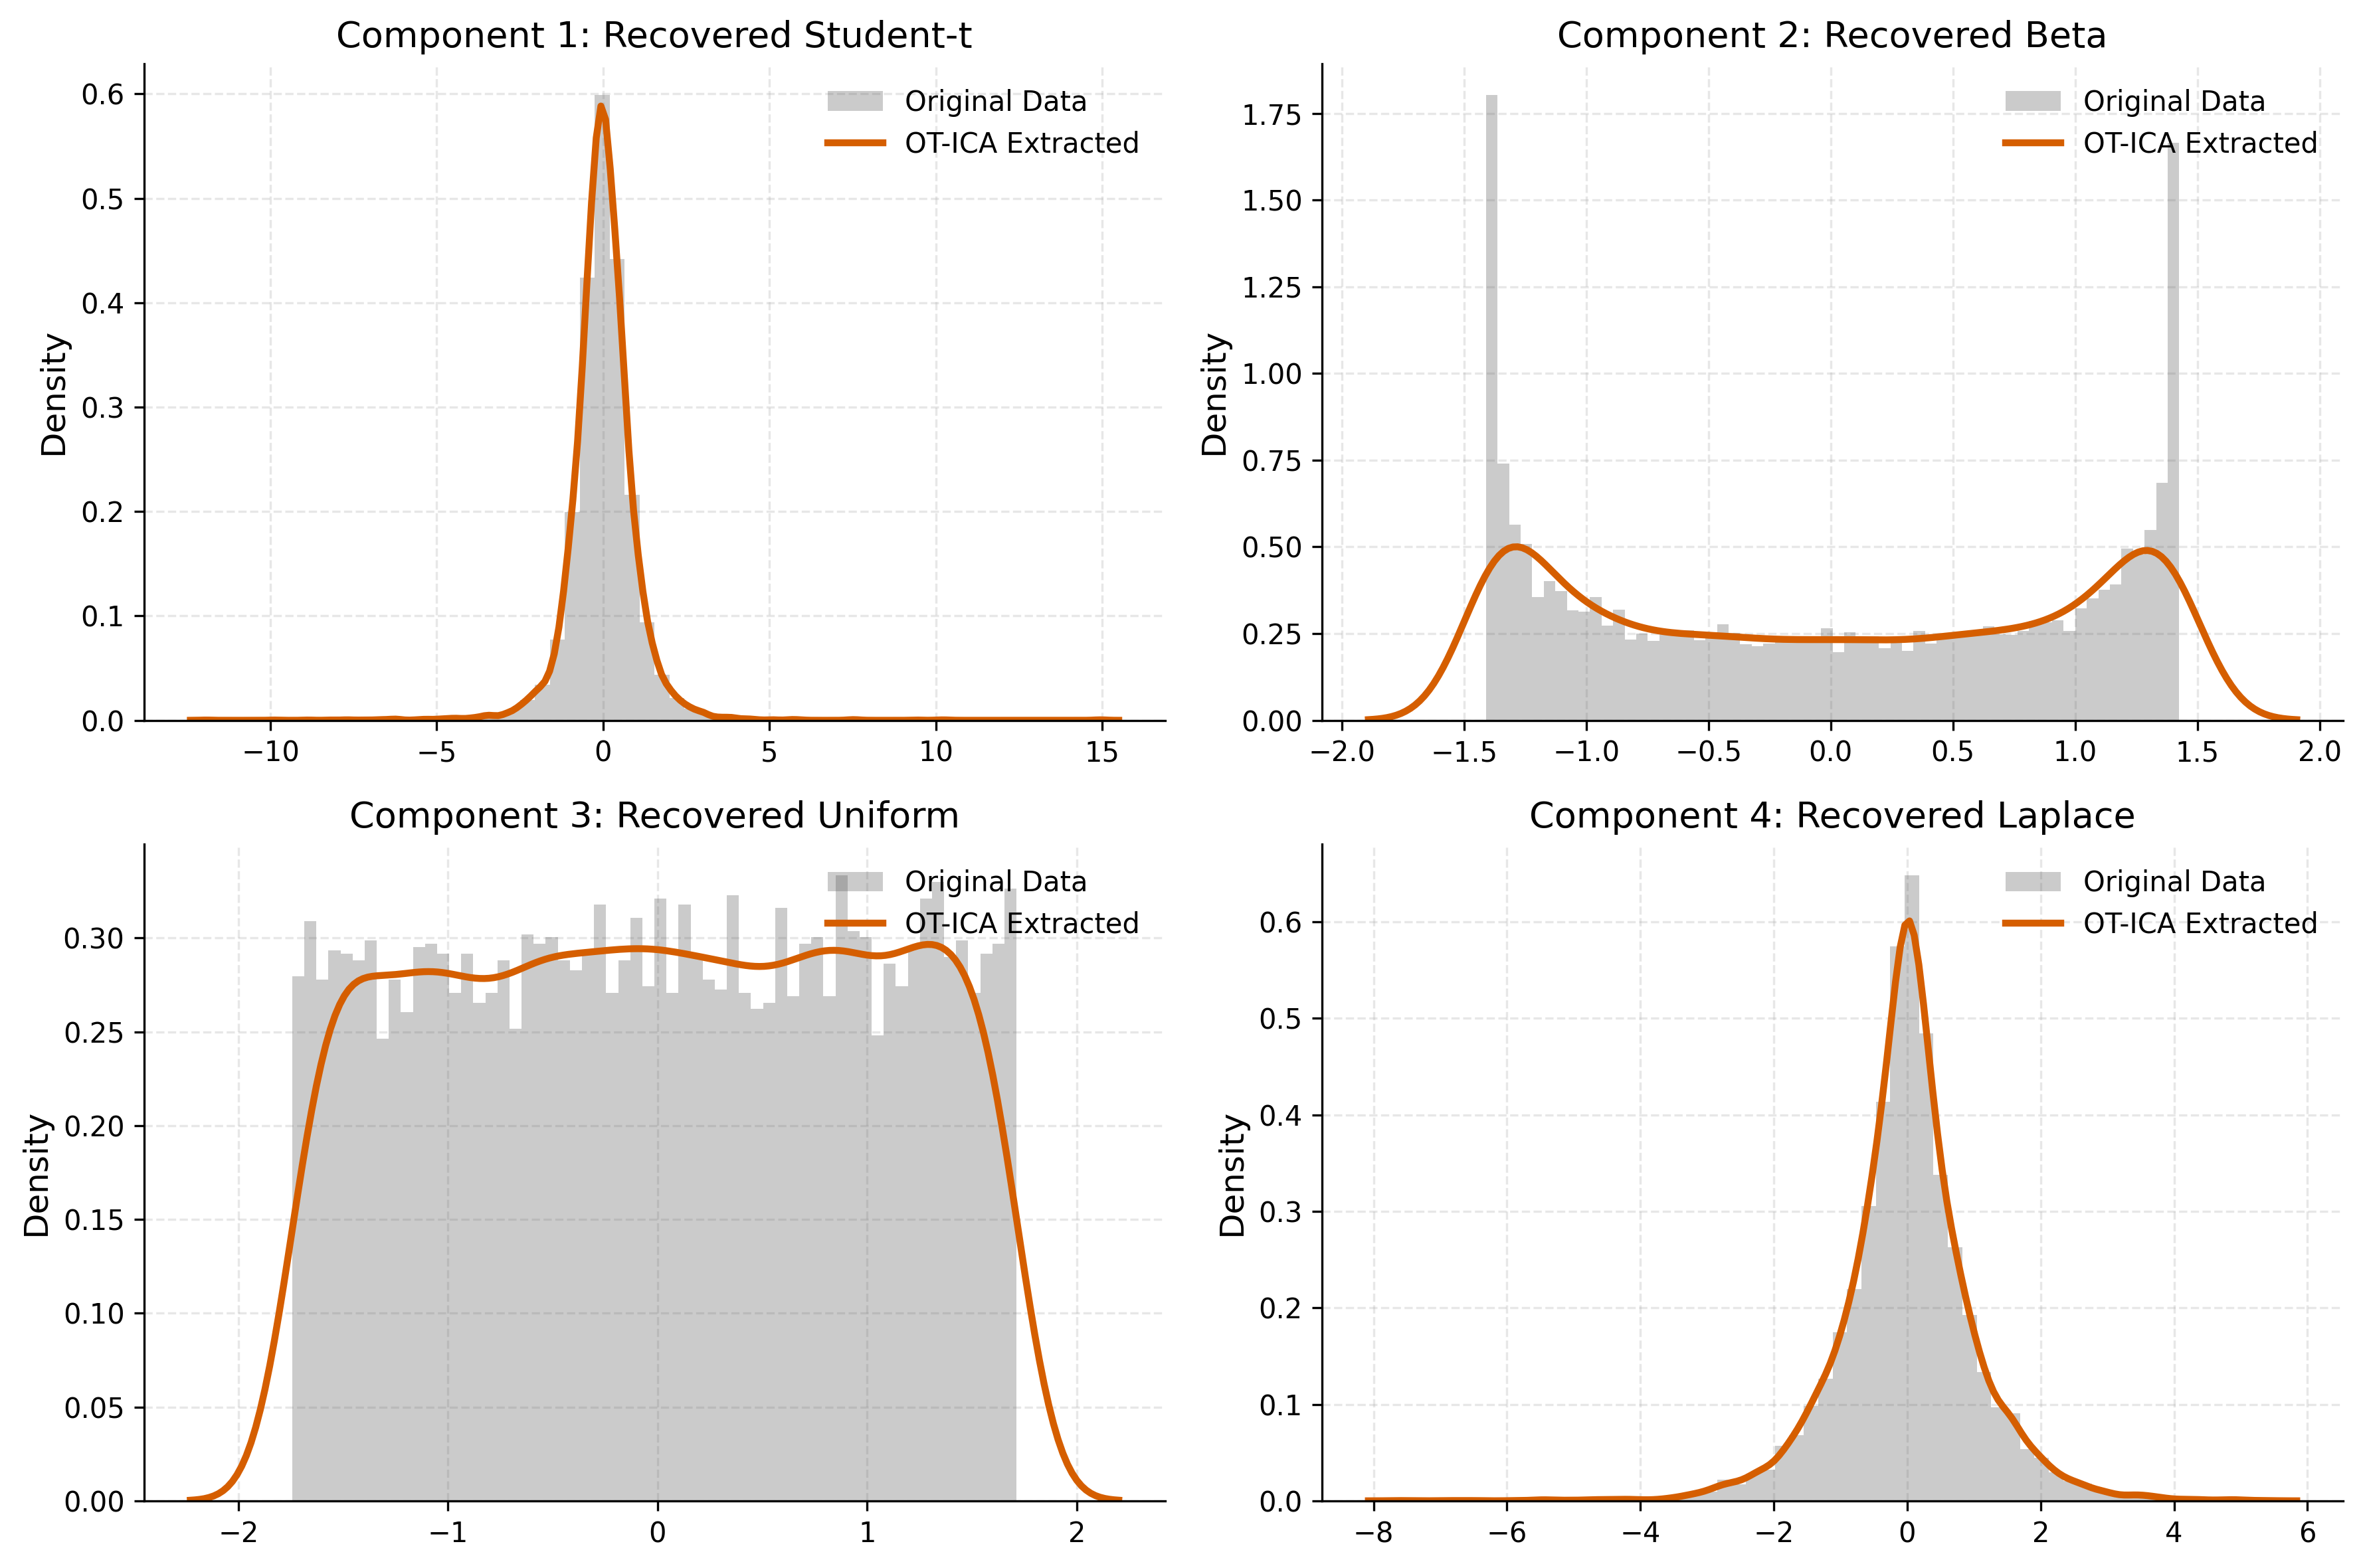
\includegraphics[width=1.0\textwidth]{otica_baseline_recovery.png} 
    \caption[Baseline Source Recovery via OT-ICA]{Empirical probability distributions of the 4D baseline validation. 
    The original generated sources are represented by gray histograms, overlaid with the sources extracted by the OT-ICA algorithm (orange curves). 
    The framework successfully reconstructs a diverse array of continuous non-Gaussian structures, easily navigating both super-Gaussian peaks and sub-Gaussian bimodality.}
    \label{fig:otica_baseline_recovery}
\end{figure}

As visualized in Figure \ref{fig:otica_baseline_recovery}, the OT-ICA algorithm flawlessly extracted all four structural signals from the mixture. 
To quantify this separation numerically, we compare the true mixing matrix $\mathbf{A}$, the estimated unmixing matrix $\mathbf{W}_{\text{est}}$, 
and the resulting global transfer matrix $\mathbf{P} = \mathbf{W}_{\text{est}}\mathbf{A}$. Because ICA is subject to inherent permutation and sign ambiguities, 
directly inferring the quality of separation by visually comparing the estimated unmixing matrix 
to the true mixing matrix is difficult, as the recovered components will be scrambled and randomly sign-flipped. 
To definitively prove the unmixing succeeded, we rely on the global transfer matrix $\mathbf{P}$. If the algorithm successfully inverted the mixing process, 
$\mathbf{P}$ collapses into a generalized permutation matrix, containing exactly one dominant absolute value near $1.0$ per row and column, with all other cross-mixing elements near zero.

\begin{table}[tbp]
    \centering
    \small
    \begin{tabular}{cc}
        \toprule
        \textbf{True Mixing Matrix ($\mathbf{A}$)} & \textbf{Estimated Unmixing Matrix ($\mathbf{W}_{\text{est}}$)} \\
        \midrule
        $
        \begin{bmatrix}
         1.058 &  1.520 & -0.249 &  1.012 \\
         0.042 & -0.486 &  0.388 & -0.523 \\
        -0.154 & -1.572 & -0.304 & -1.234 \\
        -0.006 &  0.503 &  0.053 &  0.928 
        \end{bmatrix}
        $ 
        & 
        $
        \begin{bmatrix}
         0.154 & -1.943 &  0.608 & -0.456 \\
        -0.092 & -0.284 & -0.632 & -1.977 \\
         0.146 &  0.719 &  1.097 &  1.691 \\
         1.021 &  1.204 &  0.828 &  0.677 
        \end{bmatrix}
        $ \\
        \midrule
        \multicolumn{2}{c}{\textbf{Global Transfer Matrix ($\mathbf{P} = \mathbf{W}_{\text{est}}\mathbf{A}$)}} \\
        \midrule
        \multicolumn{2}{c}{
        $
        \begin{bmatrix}
        -0.010 & -0.007 & -1.000 & -0.002 \\
         0.000 & -0.003 &  0.000 & -1.000 \\
         0.006 & -1.000 & -0.002 & -0.012 \\
         1.000 &  0.006 & -0.003 &  0.010 
        \end{bmatrix}
        $
        } \\
        \midrule
        \multicolumn{2}{c}{\textbf{Amari Performance Index}} \\
        \midrule
        \multicolumn{2}{c}{OT-ICA Error: \textbf{0.0155} \quad | \quad FastICA Error: \textbf{0.0188}} \\
        \bottomrule
    \end{tabular}
    \caption[Baseline Matrices and Amari Error]{The ground truth mixing matrix, estimated unmixing matrix, and resulting global transfer matrix for the OT-ICA baseline validation. 
    The transfer matrix closely approximates a generalized permutation matrix, visually proving successful separation alongside the comparable Amari error to FastICA.}
    \label{tab:baseline_matrices}
\end{table}

As demonstrated in Table \ref{tab:baseline_matrices}, the global transfer matrix $\mathbf{P}$ forms a near-perfect generalized permutation matrix, 
containing exactly one dominant absolute value per row and column. This confirms that OT-ICA successfully extracted the original independent sources, 
achieving an excellent Amari error well below the critical $0.1$ threshold. For comparison, we evaluated the industry-standard FastICA algorithm 
(with a \textit{logcosh} contrast function) on the exact same 4D mixture. FastICA also successfully separated the sources, achieving a highly comparable Amari error.

\section{Computational \& Temporal Scaling}
Having established that OT-ICA successfully recovers independent sources from linear mixtures in low dimensions, we must evaluate its computational scaling in high-dimensional cases. 
We benchmarked OT-ICA against FastICA, utilizing a linear mixture of continuous super-Gaussian Laplacian sources. 
We evaluated both algorithms across increasing dimensions with a fixed sample size of $N=10,000$. Because OT-ICA relies on gradient-based optimization over the Stiefel manifold, 
its capacity to find global optima depends on computational resources in higher dimensions. Therefore, we evaluated both algorithms under the predefined Low Compute and High Compute regimes (defined in Table \ref{tab:compute_regimes}).

\begin{figure}[tbp]
    \centering
    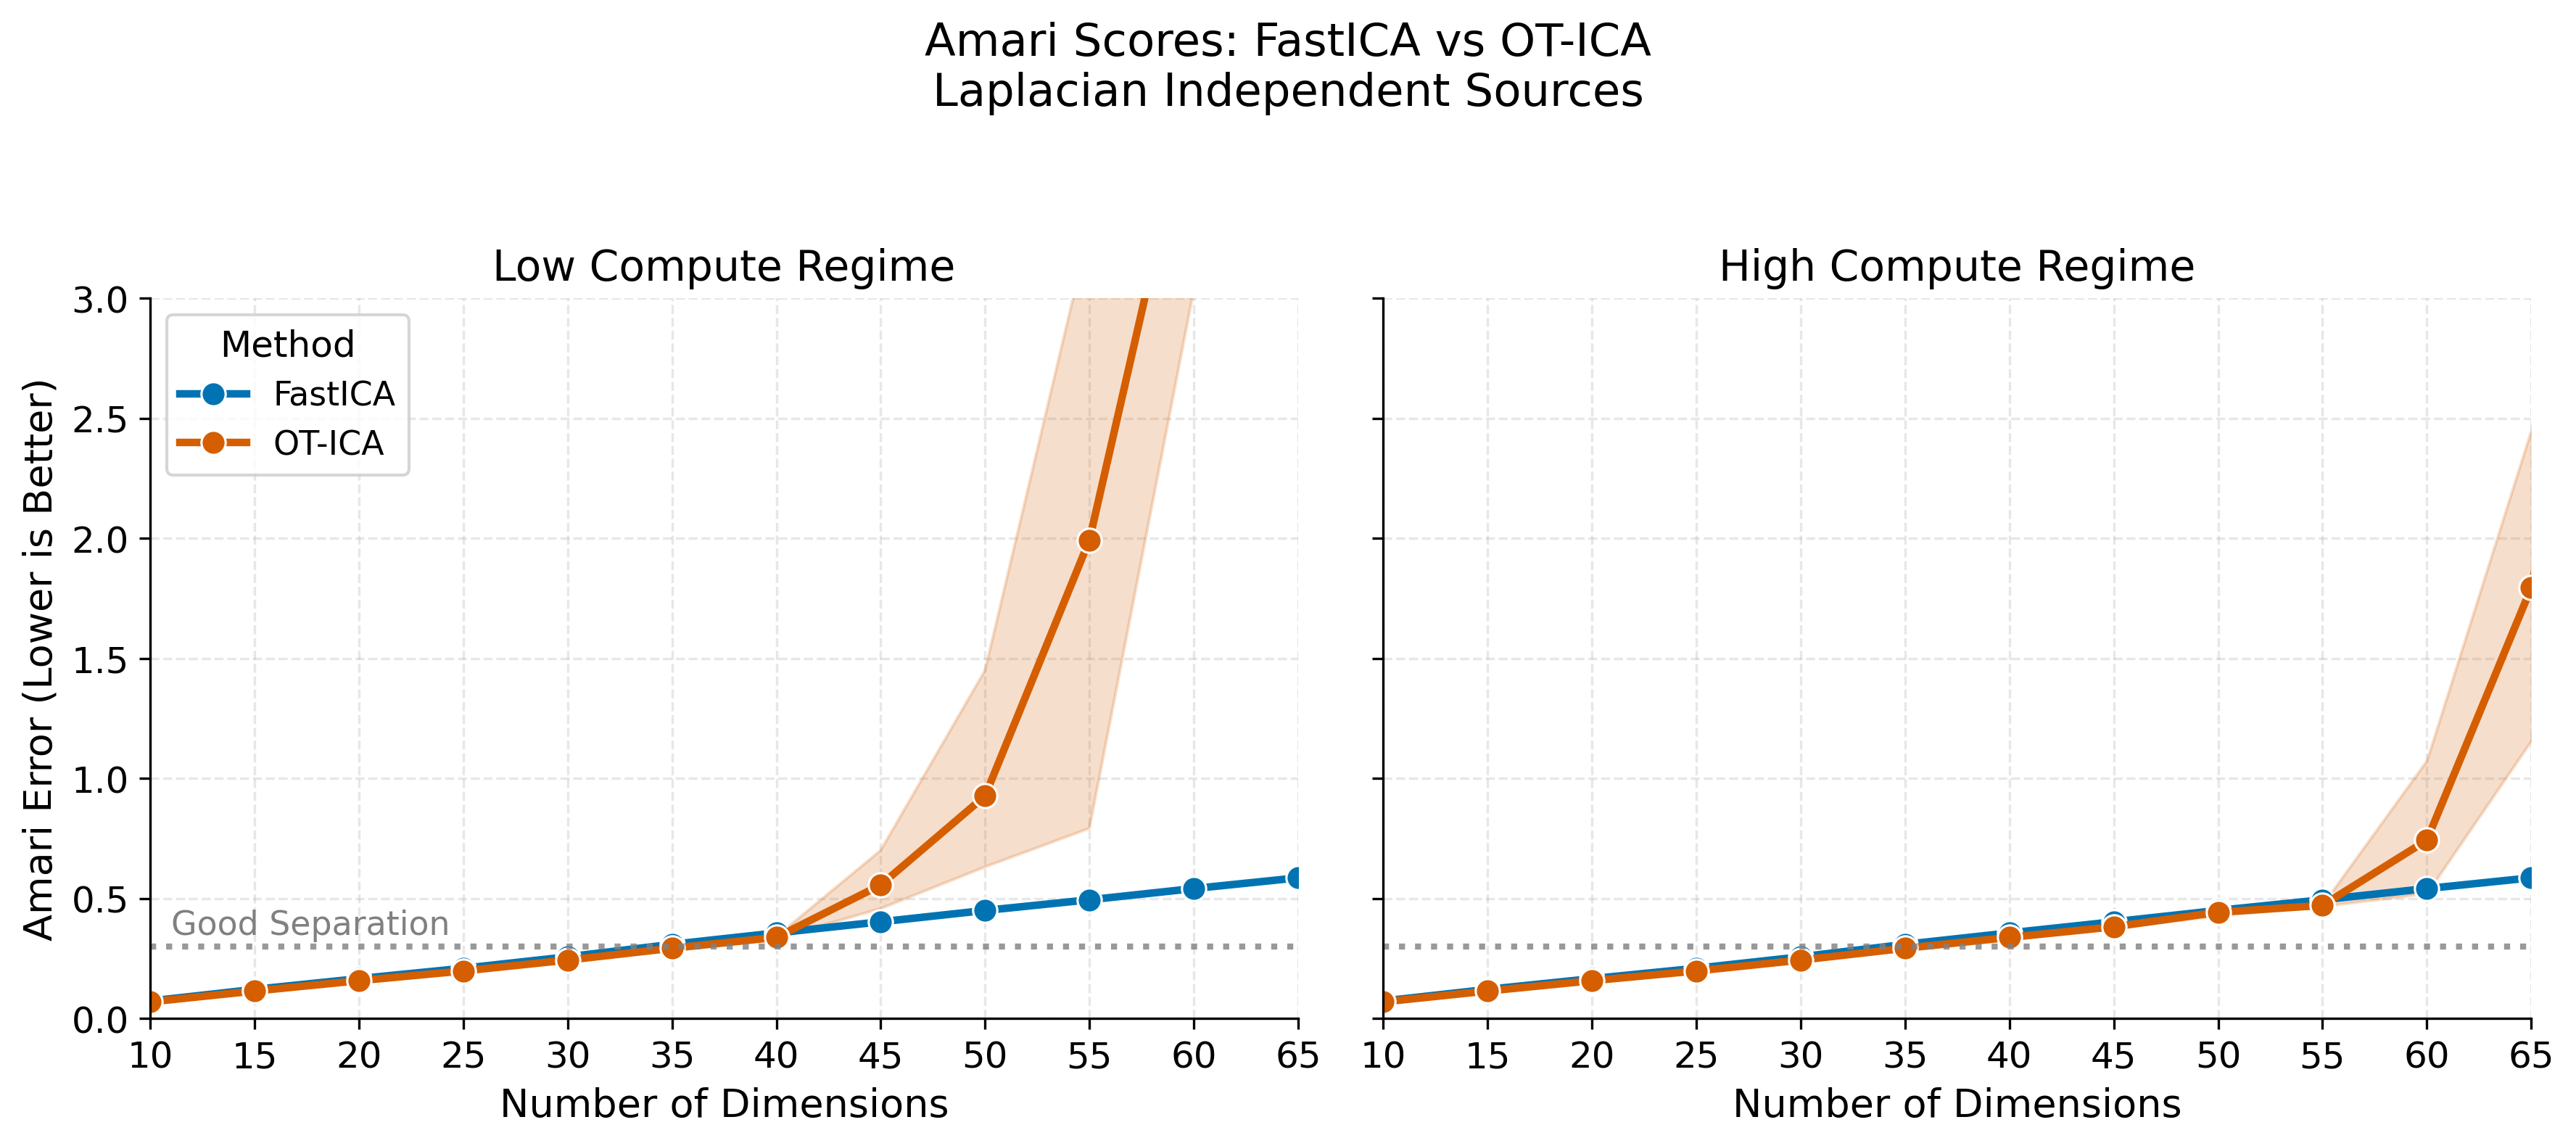
\includegraphics[width=1.0\textwidth]{laplace_amari_ot_ica_scaling.png} 
    \caption[Separation Accuracy on Laplacian Sources]{Amari error comparison between FastICA and OT-ICA across increasing dimensions for standard Laplacian sources. While OT-ICA degrades in the Low Compute regime due to the expanding surface area of the Stiefel manifold, the High Compute regime successfully restores accurate separation ($E < 0.3$), matching FastICA's capabilities up until the absolute dimensionality limit.}
    \label{fig:laplace_amari_scaling}
\end{figure}

As shown in Figure \ref{fig:laplace_amari_scaling}, FastICA performs exceptionally well in this standard environment for lower dimensions, 
maintaining near-perfect separation regardless of the compute regime. This is expected, as the Laplacian distribution perfectly aligns with FastICA's 
default \textit{logcosh} proxy contrast function. Conversely, while OT-ICA successfully scales alongside FastICA, 
it strictly requires the High Compute regime to overcome the expanding complexity of the high dimension optimization landscape. 
However, this experiment also reveals a fundamental absolute ceiling. As the dimensionality approaches and exceeds $d=40$, 
the curse of dimensionality overtakes the fixed sample size ($N=10,000$). At this extreme, the statistical resolution of the joint distribution degrades so severely 
that both algorithms, regardless of the computational power, fail to maintain the "Good Separation" threshold ($E < 0.3$). 
This shared degradation highlights the fundamental trade-off between sample size and dimensionality, demonstrating a statistical limit of the data rather than an isolated algorithmic defect.

\begin{figure}[tbp]
    \centering
    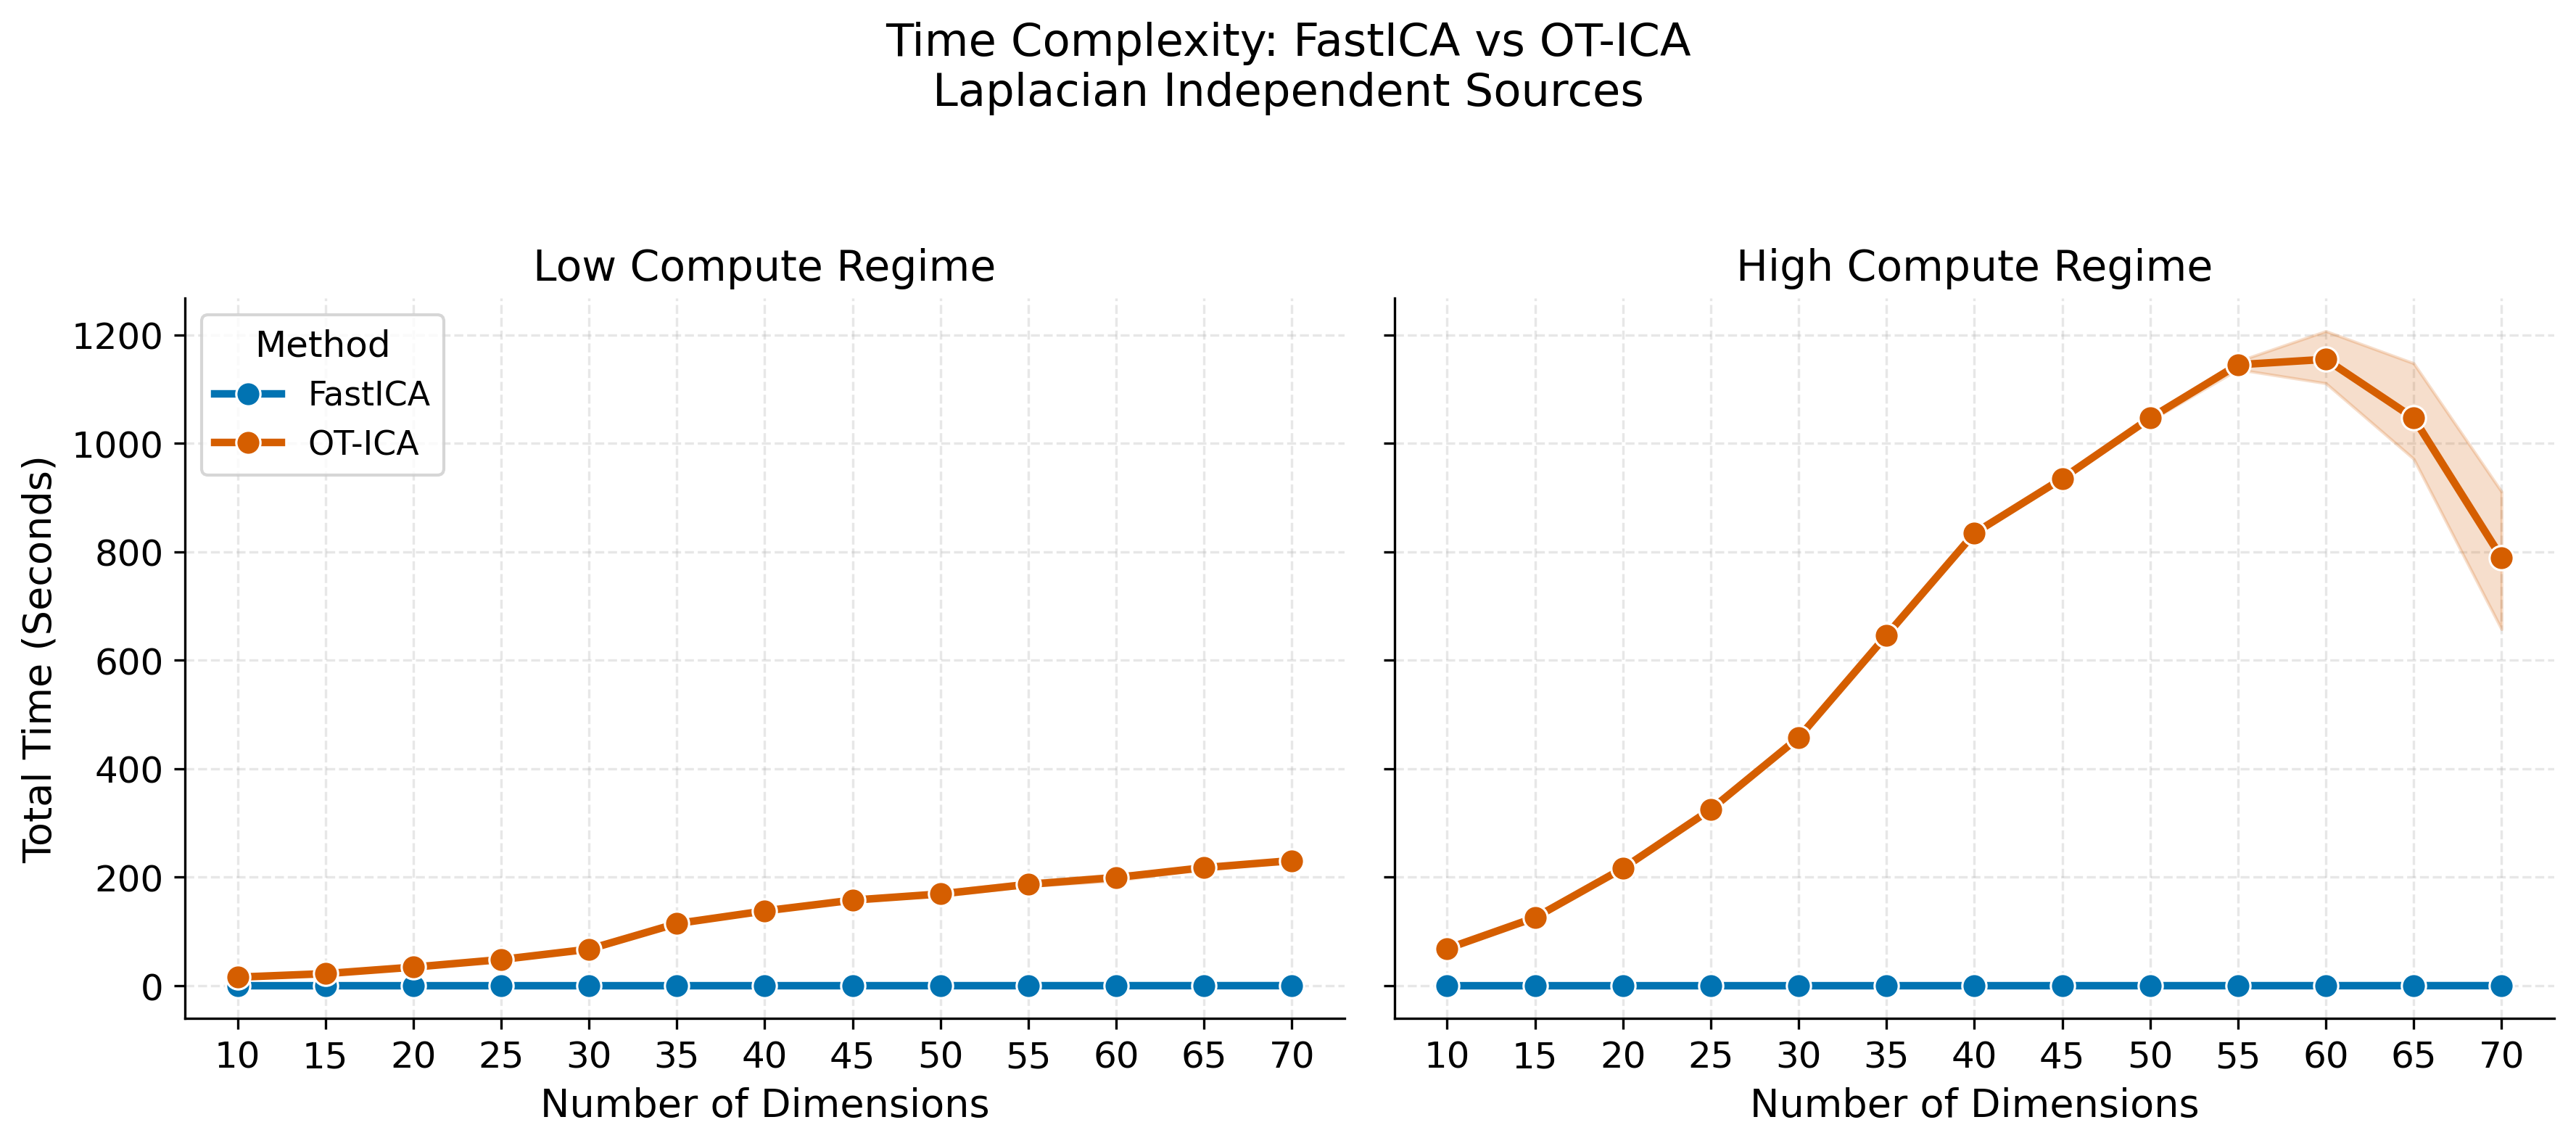
\includegraphics[width=1.0\textwidth]{laplace_time_ot_ica_scaling.png} 
    \caption[Execution Time Scaling]{Total execution time (in seconds) for FastICA and OT-ICA as dimensions increase, separated by compute regime. 
    OT-ICA exhibits exponentially higher computational costs, particularly in the High Compute regime (right) where dense parallel restarts are required to maintain performance.}
    \label{fig:laplace_time_scaling}
\end{figure}

Crucially, as illustrated in Figure \ref{fig:laplace_time_scaling}, the computational cost required for OT-ICA to remain competitive before hitting 
the dimensionality ceiling is orders of magnitude higher than FastICA. FastICA's Newton-based fixed-point iteration allows it to converge in fractions of a second. 
In contrast, OT-ICA's first-order gradient descent and required parallel restarts cause execution times to scale steeply, taking significantly longer to achieve the same result.
This stark disparity in algorithmic efficiency poses a critical question: 
\textit{If FastICA is computationally instantaneous, and mathematically highly accurate up to the exact same statistical ceiling on standard distributions, 
why develop and utilize a computationally expensive gradient based framework like OT-ICA?}

The answer lies in the fragility of proxy-based Newton solvers. While FastICA perfectly separates the homogeneous mixture of continuous distributions shown above, 
real-world data is frequently heterogeneous in nature. In the following sections, we demonstrate how agorithmic assumptions trigger failures for FastICA in generalized mixtures, 
and how the global geometry of OT-ICA natively bypasses these blind spots.

\section{The Blind Spots of FastICA}
In this section, we present two distinct mathematical blind spots that cause FastICA to fail on non-Gaussian independent components due to 
it's reliance on proxy contrast functions and Newton-based Fixed point iteration method.

\subsection{The Zero Negentropy Pitfall}
FastICA does not measure true negentropy; instead, it relies on a computationally efficient approximation. For a whitened random variable $x$, 
the negentropy $J(x)$ is approximated using a non-quadratic contrast function $G(\cdot)$, most commonly the \textit{logcosh} function $G(x) = \frac{1}{a} \log \cosh(ax)$. 
The approximation is given by:
\begin{equation}
    J(x) \propto \big( \mathbb{E}[G(x)] - \mathbb{E}[G(\nu)] \big)^2
\end{equation}
where $\nu$ is a standard Gaussian random variable. The algorithm searches for projections that maximize this squared difference. 

The first failure mode occurs if a latent independent source possesses a specific structural shape such that its expected value under the 
contrast function exactly equals that of a Gaussian, i.e., $\mathbb{E}[G(x)] = \mathbb{E}[G(\nu)]$. When this equality holds, 
the approximated negentropy evaluates to zero. In this scenario, the objective function collapses. 
FastICA becomes entirely blind to the non-Gaussianity of the source, failing to extract it.

\subsection{Empirical Results: The Zero Negentropy Pitfall}
To empirically demonstrate this pitfall, we constructed a specific non-Gaussian distribution to trigger 
the zero-negentropy condition. Utilizing a symmetric Trimodal Gaussian Mixture parameterized by peak locations $\{-b, 0, b\}$ and 
variance $\sigma^2$, we solved for the peak locations and probability mass such that the expected value of 
the \textit{logcosh} function exactly matched the theoretical baseline of a standard normal distribution ($\mathbb{E}[G(x)] = \mathbb{E}[G(\nu)]$). 
Because this engineered distribution strictly maintains unit variance, it represents a valid, independent non-Gaussian source 
that is theoretically invisible to the FastICA contrast function.

To evaluate the algorithmic resilience of both FastICA and OT-ICA, we generated linear mixtures of this engineered Trimodal Gaussian source 
across increasing dimensions ($d \in [5, 25]$) with a fixed sample size of $N=10,000$. 
To cleanly isolate fundamental mathematical blindness from standard non-convex optimization difficulty, 
we separated the evaluation into the predefined Low Compute and High Compute regimes (see Table \ref{tab:compute_regimes}).

\begin{figure}[tbp]
    \centering
    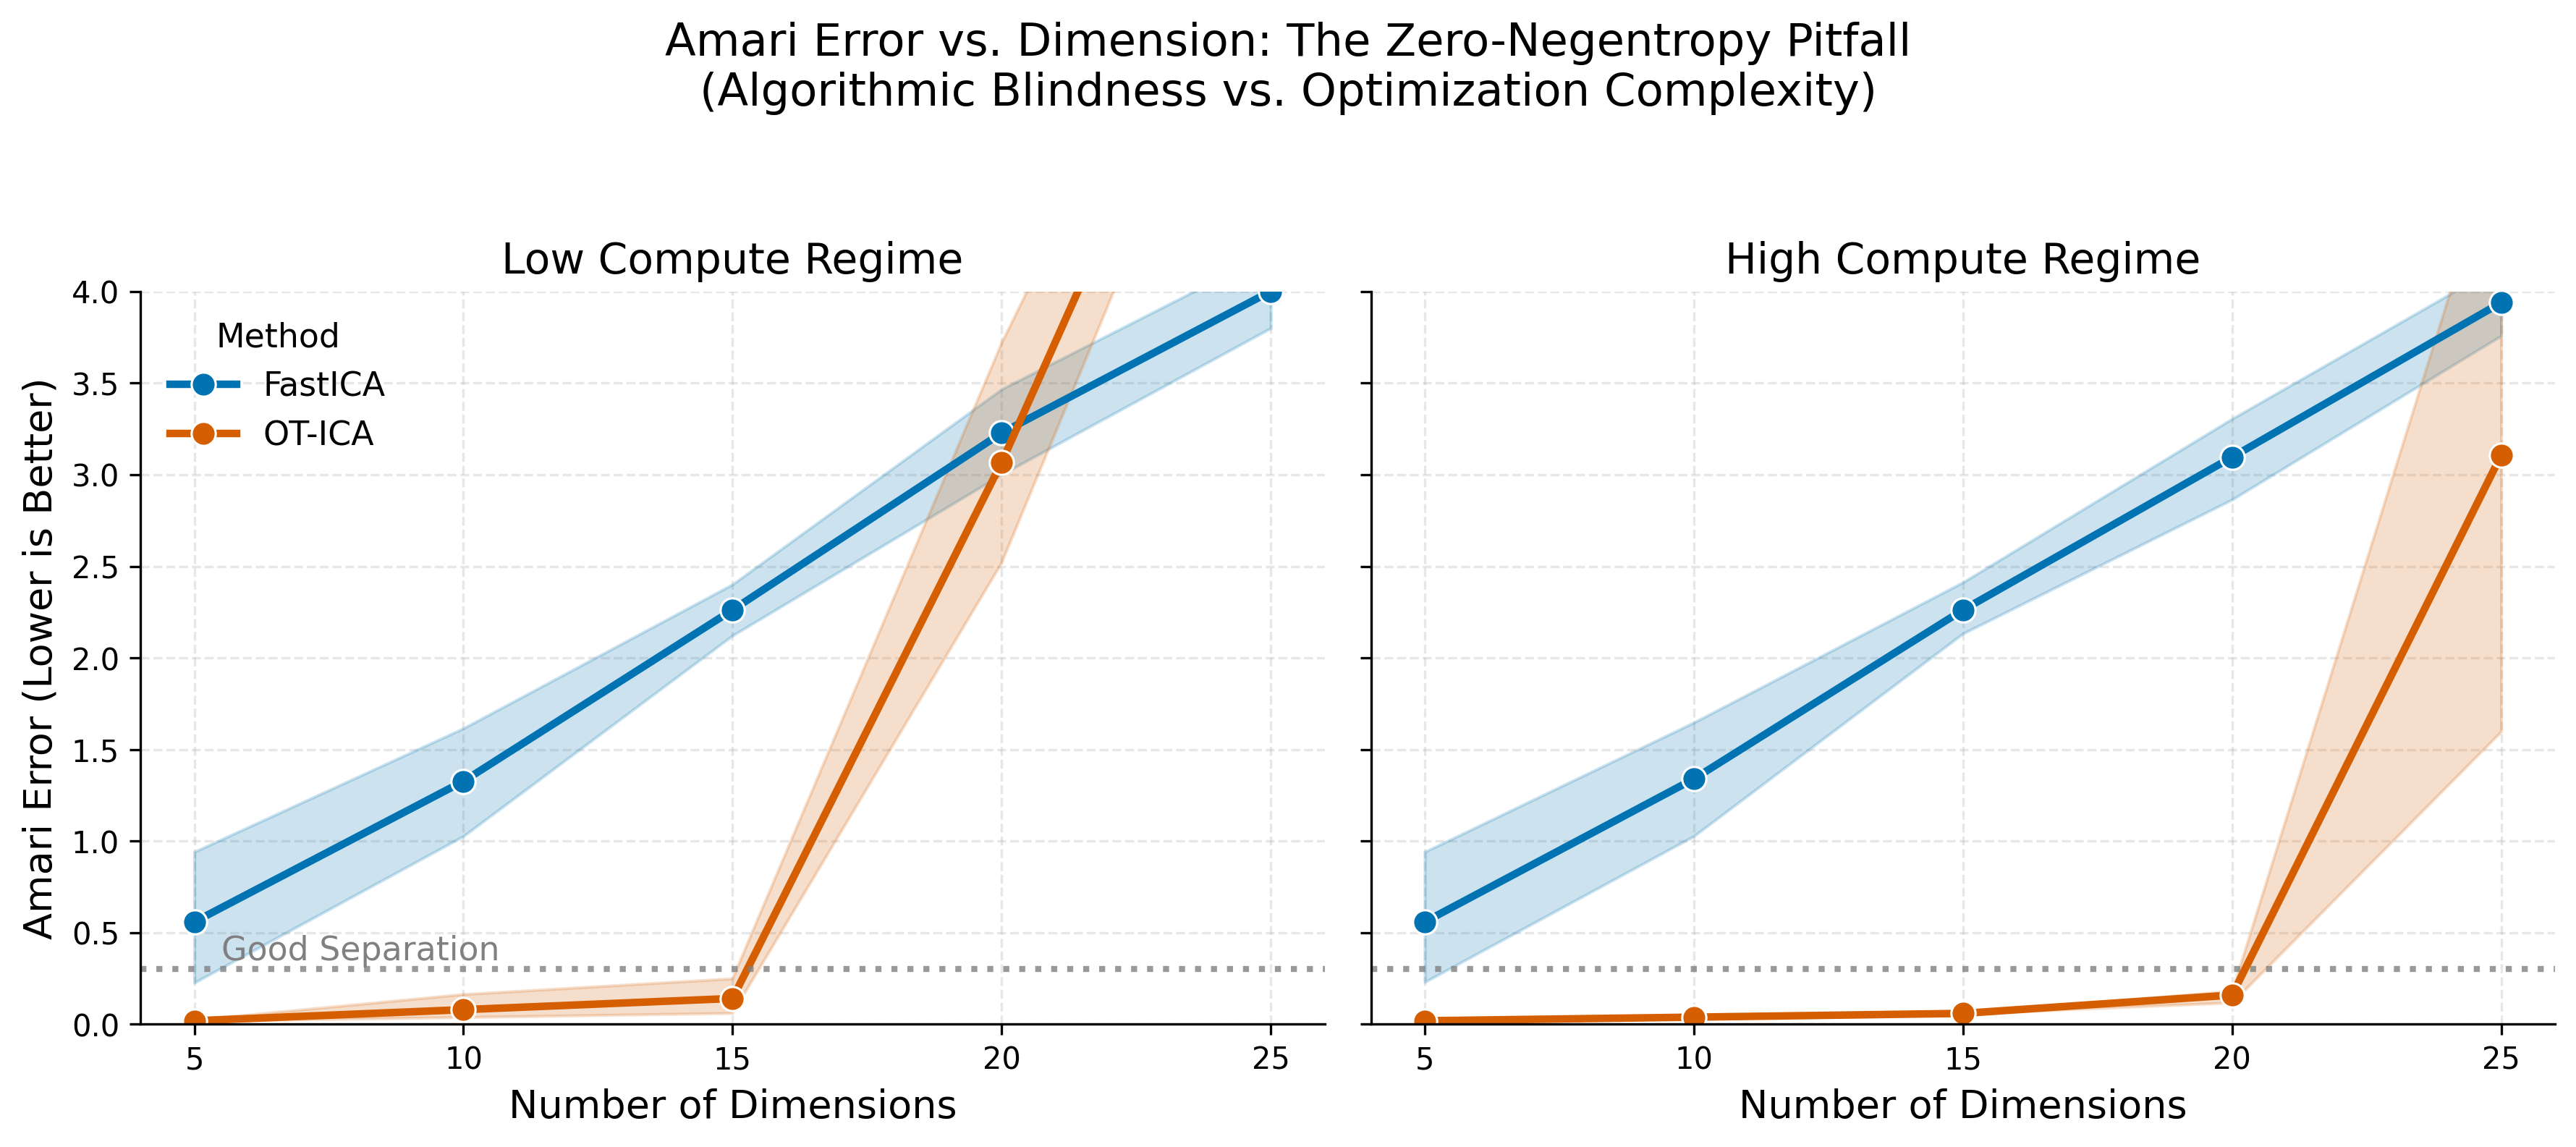
\includegraphics[width=1.0\textwidth]{zero_negentropy_amari_compute.png} 
    \caption[Performance on Zero-Negentropy Failure Mode]{Amari error comparison between FastICA and OT-ICA for the engineered 
    zero-negentropy Trimodal Gaussian distribution. FastICA experiences failure ($E > 0.5$) across all regimes due to algorithmic blindness. 
    OT-ICA successfully unmixes the sources, but depends on high compute regime for higher dimension cases.}
    \label{fig:zero_negentropy_amari}
\end{figure}

As illustrated in Figure \ref{fig:zero_negentropy_amari}, the empirical results validate the mathematical collapse of FastICA. 
Because this engineered Trimodal Gaussian generates a proxy negentropy of exactly zero, FastICA falsely perceives 
the independent source as indistinguishable from standard Gaussian noise. Consequently, the algorithm completely fails to separate the mixtures, 
consistently returning high Amari errors ($E>0.5$). Providing FastICA with High Compute resources yields no improvement; 
this confirms that the failure is strictly structural, a fundamental mathematical blind spot inherent to the proxy-based solver.

In contrast, the OT-ICA framework demonstrates robust source separation until the trade-off between a fixed sample size 
and dimensional complexity emerges. This stability is achieved by completely bypassing parametric approximations and instead mapping 
the full global geometry of the empirical Cumulative Distribution Function (CDF) via Optimal Transport.

While OT-ICA experiences performance degradation in the Low Compute regime at $d>15$, this is a symptom of the exponentially expanding, 
highly non-convex surface area of the Stiefel manifold, not a failure of the objective function. When provided with dense parallel restarts in 
the High Compute regime, OT-ICA successfully navigates the complex search space and restores accurate unmixing ($E<0.3$) untill $d=20$. 
This empirically reaffirms that while OT-ICA is bound by computational search complexity, it fundamentally resolves 
the zero-negentropy mathematical blind spot of FastICA.

\subsection{The Vanishing Curvature Pitfall}
The \textit{optimization algorithm} used by FastICA utilizes a Newton (second-order) fixed-point iteration step to achieve super-linear convergence. 
However, the mathematical stability of this convergence relies explicitly on a foundational technical assumption governing 
the algorithmic curvature of the optimization landscape. As formalized in the FastICA convergence proofs 
by Hyv{\"a}rinen, Karhunen, and Oja \cite[Chapter 8]{hyvarinen2001} (reproduced in Appendix \ref{app:fastica_proof}), 
this requirement is dictated by the following expectation:

The proof states that for the fixed-point iteration to converge to a true independent component $s_i$, 
the expected value governing the second-order Taylor expansion of the iteration must not vanish. 
Specifically, defining $g(x) = G'(x)$ and $g'(x) = G''(x)$, where $G$ is the contrast function, the convergence requires:
\begin{equation}
    \mathbb{E}\big[s_i g(s_i) - g'(s_i)\big] \neq 0
\end{equation}
This expectation geometrically represents the algorithmic curvature of the optimization landscape at the optimal point. 
For the standard \textit{logcosh} contrast function (with $a=1$), this equates to $g(x) = \tanh(x)$ and $g'(x) = 1 - \tanh^2(x)$. 

If a specific non-Gaussian source distribution naturally causes this specific expectation to evaluate precisely to zero, 
the algorithmic curvature vanishes. When this condition fails, the denominator of the FastICA update rule collapses, 
negating the local quadratic (or cubic) convergence guarantees. The fixed-point iteration fails to converge, 
even though the component is strictly independent and non-Gaussian.

\subsection{Empirical Results: The Vanishing Curvature Pitfall}
To empirically demonstrate the vanishing curvature limitation, we engineered a continuous source distribution specifically designed to trigger the assumption 
described in the previous section. 
We analyzed the target function representing the curvature condition: 
\begin{equation}
    h(x) = x \tanh(x) - 1 + \tanh^2(x).
\end{equation}
We observed that $h(x)$ evaluates to negative values near the origin ($|x| < 0.82$) and positive values in the extreme tails. 

We constructed a Trimodal Gaussian Mixture model parameterized by symmetrically spaced peak locations $\{-b, 0, b\}$ and a shared variance $\sigma^2$. 
By solving the integral equation $\int h(x) \text{PDF}(x) dx = 0$ subject to the standard unit variance constraint ($\mathbb{E}[X^2] = 1$), 
we determined the exact probability masses required to perfectly balance the negative central region against the positive tail regions. 

\begin{figure}[tbp]
    \centering
    
\includegraphics[width=0.85\textwidth]{vanishing_curvature_trimodal_pdf.png} 
    \caption[The Vanishing Curvature Counterexample]{The engineered Trimodal Gaussian Mixture designed to illustrate 
    the vanishing curvature pitfall in FastICA. The central mass generates negative algorithmic curvature, while 
    the side peaks (marked by red dotted lines at $\pm b$) generate positive algorithmic curvature. 
    The parameters $b$ and $p$ are computationally root-solved such that these regions perfectly cancel out ($\int h(x) \text{PDF}(x) dx = 0$) 
    while strictly maintaining unit variance, effectively hiding the non-Gaussian signal from the Newton-step solver.}
    \label{fig:vanishing_curvature}
\end{figure}

This carefully engineered distribution, illustrated in Figure \ref{fig:vanishing_curvature}, 
remains strictly non-Gaussian and perfectly valid under the linear ICA assumptions, 
yet its algorithmic curvature is exactly zero, which should render it mathematically invisible to FastICA's fixed-point solver.

To isolate fundamental mathematical failures from standard optimization difficulties, we evaluated both FastICA and OT-ICA 
across increasing dimensions ($d \in [5, 25]$) at a fixed sample size of $N=10,000$. The experiment was conducted under the 
predefined Low Compute and High Compute regimes (Table \ref{tab:compute_regimes}).

\begin{figure}[tbp]
    \centering
    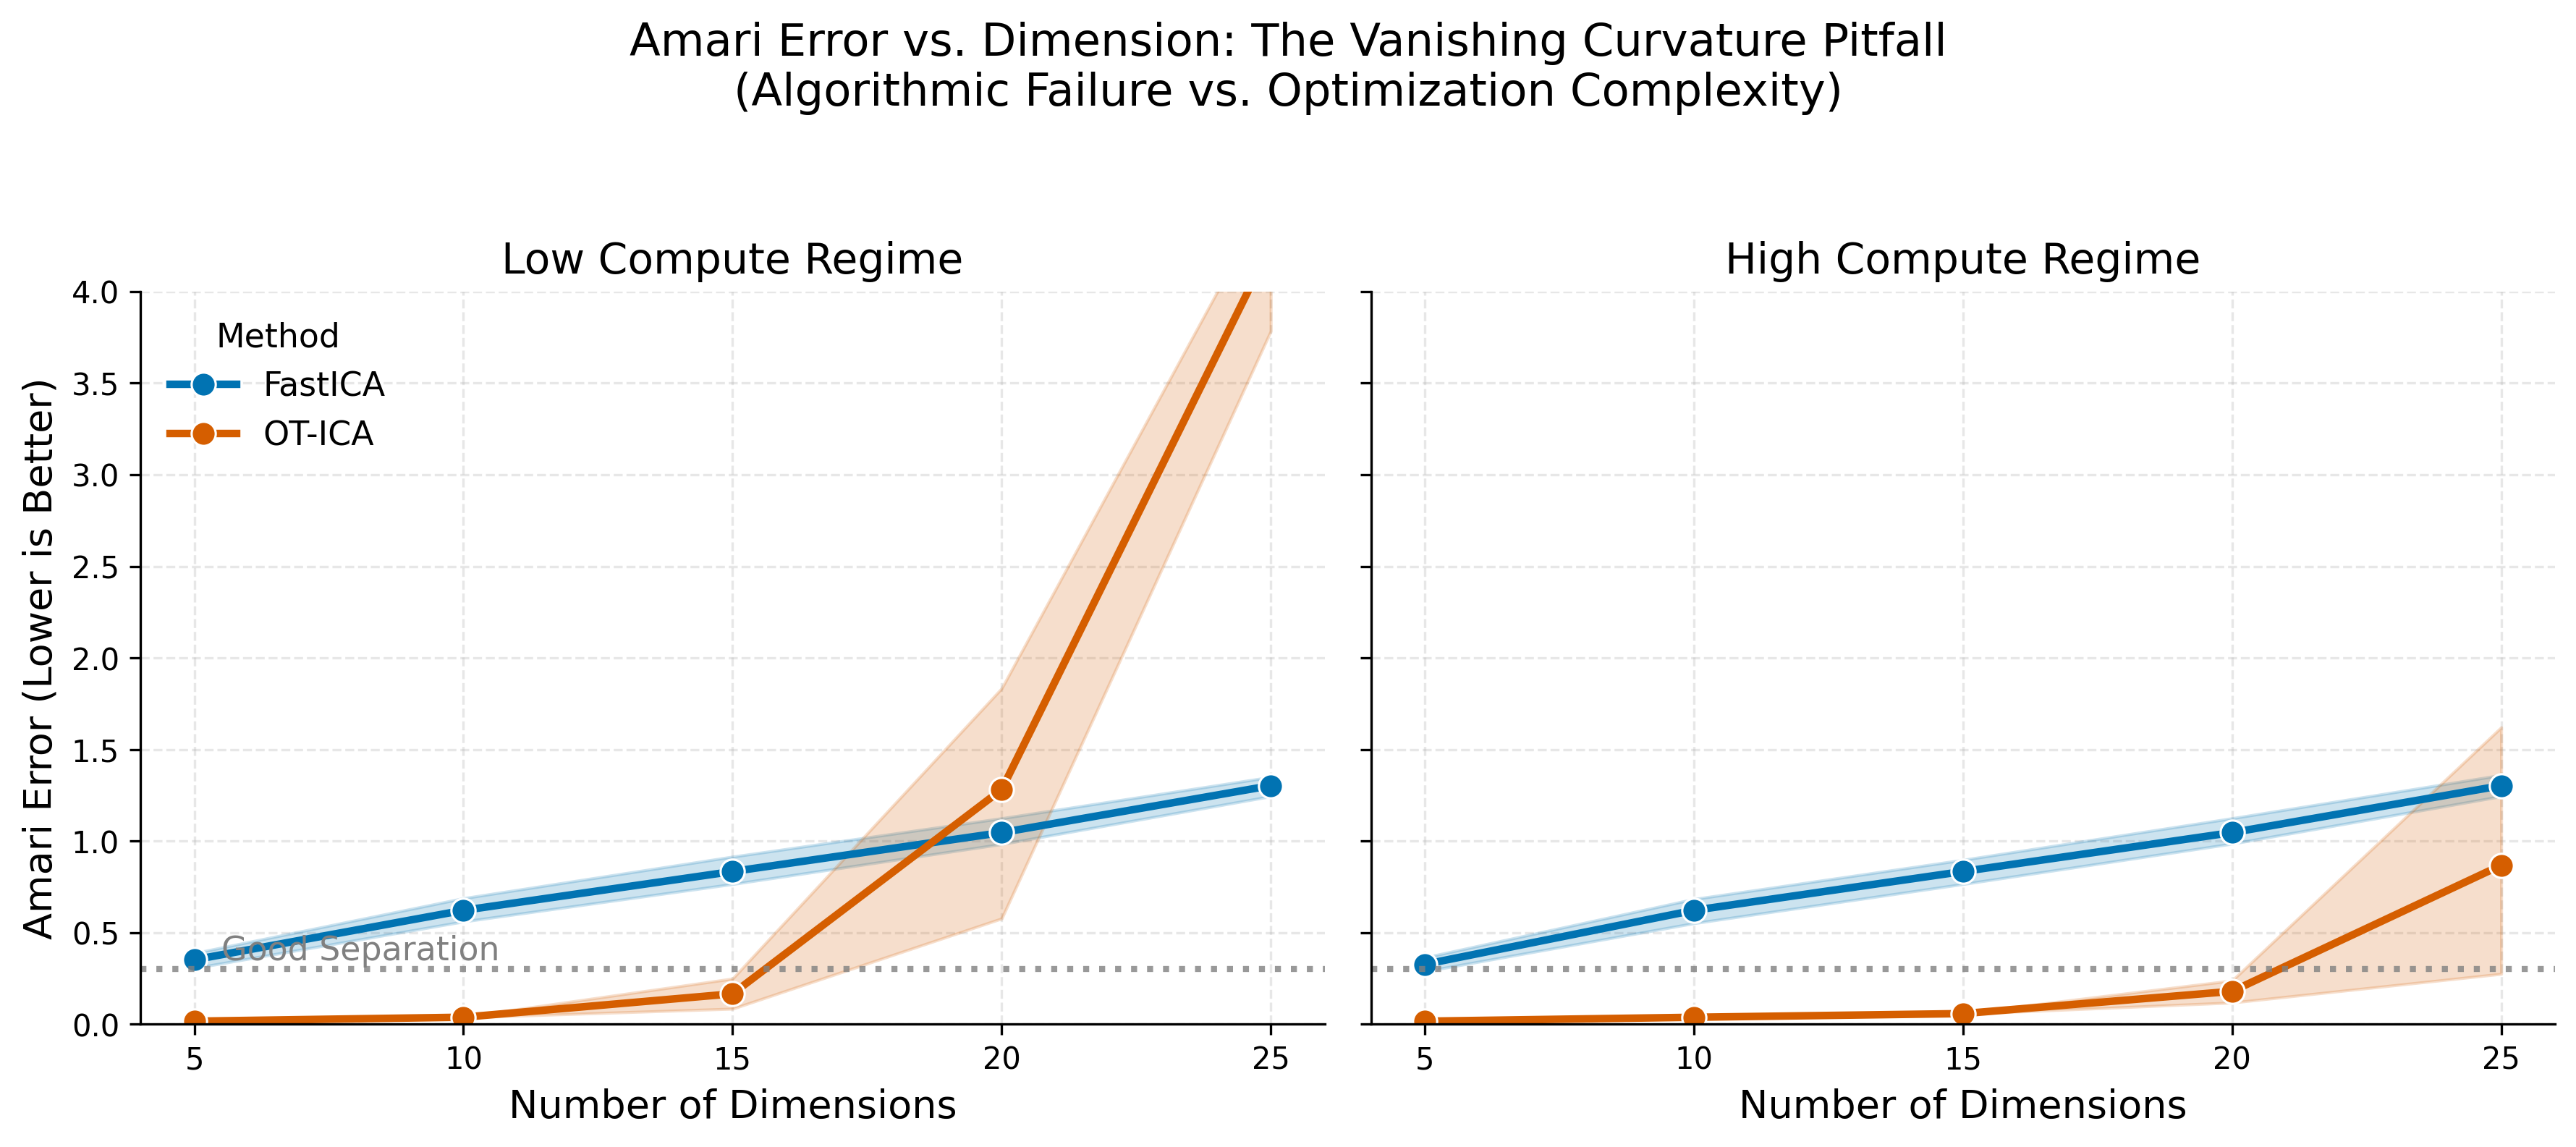
\includegraphics[width=1.0\textwidth]{vanishing_curvature_amari_compute.png} 
    \caption[Performance on Trimodal Failure Mode]{Amari error comparison between FastICA and OT-ICA across increasing dimensions for 
    the engineered Trimodal distribution. FastICA experiences catastrophic mathematical failure ($E > 1.0$) across all regimes. 
    OT-ICA's performance degradation at higher dimensions is revealed to be a non-convexity search problem, 
    as the High Compute regime successfully restores good separation.}
    \label{fig:amari_trimodal_failure}
\end{figure}

The empirical results, visualized in Figure \ref{fig:amari_trimodal_failure}, confirm a stark structural divergence between the two algorithms. 
As mathematically predicted, FastICA consistently returned unmixing matrices with high Amari errors ($E > 0.3$) for all dimensions. 
Crucially, the High Compute Regime did nothing to improve FastICA's performance. This confirms that its failure is not a matter 
of search space exploration or iteration limits, but a fundamental algorithmic breakdown; the vanishing curvature blind spot ensures that
it's Newton Solver does not converge.

Conversely, OT-ICA's behavior reveals a completely different limitation. Under the Low Compute regime, OT-ICA successfully unmixed 
lower dimensions ($d < 20$) but degraded as $d$ increased with fixed sample size of $N=10,000$. However, when shifted to the High Compute regime, 
OT-ICA's performance recovered, maintaining a good separation, Amari error ($E < 0.3$) up through 20 dimensions. This proves that OT-ICA does not 
suffer from the curvature trap. Because it evaluates the entire global geometry of the empirical CDF via Optimal Transport, 
it is mathematically immune to local density blind spots. Its performance ceiling is instead dictated by the 
\textit{Curse of Dimensionality} and non-convexity. As dimensions increase, the surface area of the Stiefel manifold expands exponentially, 
becoming littered with shallow local maxima. OT-ICA succeeds mathematically, but requires sufficient computational power (dense random restarts) 
to thoroughly search the highly non-convex optimization landscape.

\section{The Generalized Hybrid Mixture Stress Test}
Real-world signals rarely belong to a single statistical family. To test the algorithmic robustness of both OT-ICA and FastICA, 
we designed a generalized hybrid mixture.

\subsection{Experimental Setup}
We generated linear mixtures at standard high-dimensional benchmarks ($d=30$ and $d=40$), maintaining a fixed sample size of $N=10,000$. 
To satisfy the ICA identifiability constraint, exactly one source was fixed as a standard Gaussian distribution, $\mathcal{N}(0,1)$. 
The remaining $(d-1)$ independent sources were randomly drawn from a diverse pool of eight distinct distributions: 
Laplace, Bernoulli, Uniform, Student-t, Poisson, Binomial, Chi-squared, and Exponential. 

To definitively isolate structural mathematical failures from optimization timeouts, FastICA was granted an 
extended convergence limit of $10,000$ iterations for these trials, while OT-ICA utilized its standard baseline parameters (\ref{tab:compute_regimes}).

\subsection{Empirical Results: Hybrid Mixture Stress Test}
The results, visualized in Figure \ref{fig:hybrid_mixture_results}, reveal a stark divergence in the stability of the two algorithms. 
The OT-ICA framework successfully maintained moderate to good separation ($E < 0.5$) across the tested dimensions for all but discrete only mixtures. 
This validates that the $W_2$ metric, smoothed via dithering and regularized via stochastic mini-batching, 
generalizes well across hybrid mixtures with baseline compute resources (Table \ref{tab:compute_regimes}), discrete only mixtures present 
a unique challenge that we will explore in the next section.

\begin{figure}[tbp]
    \centering
    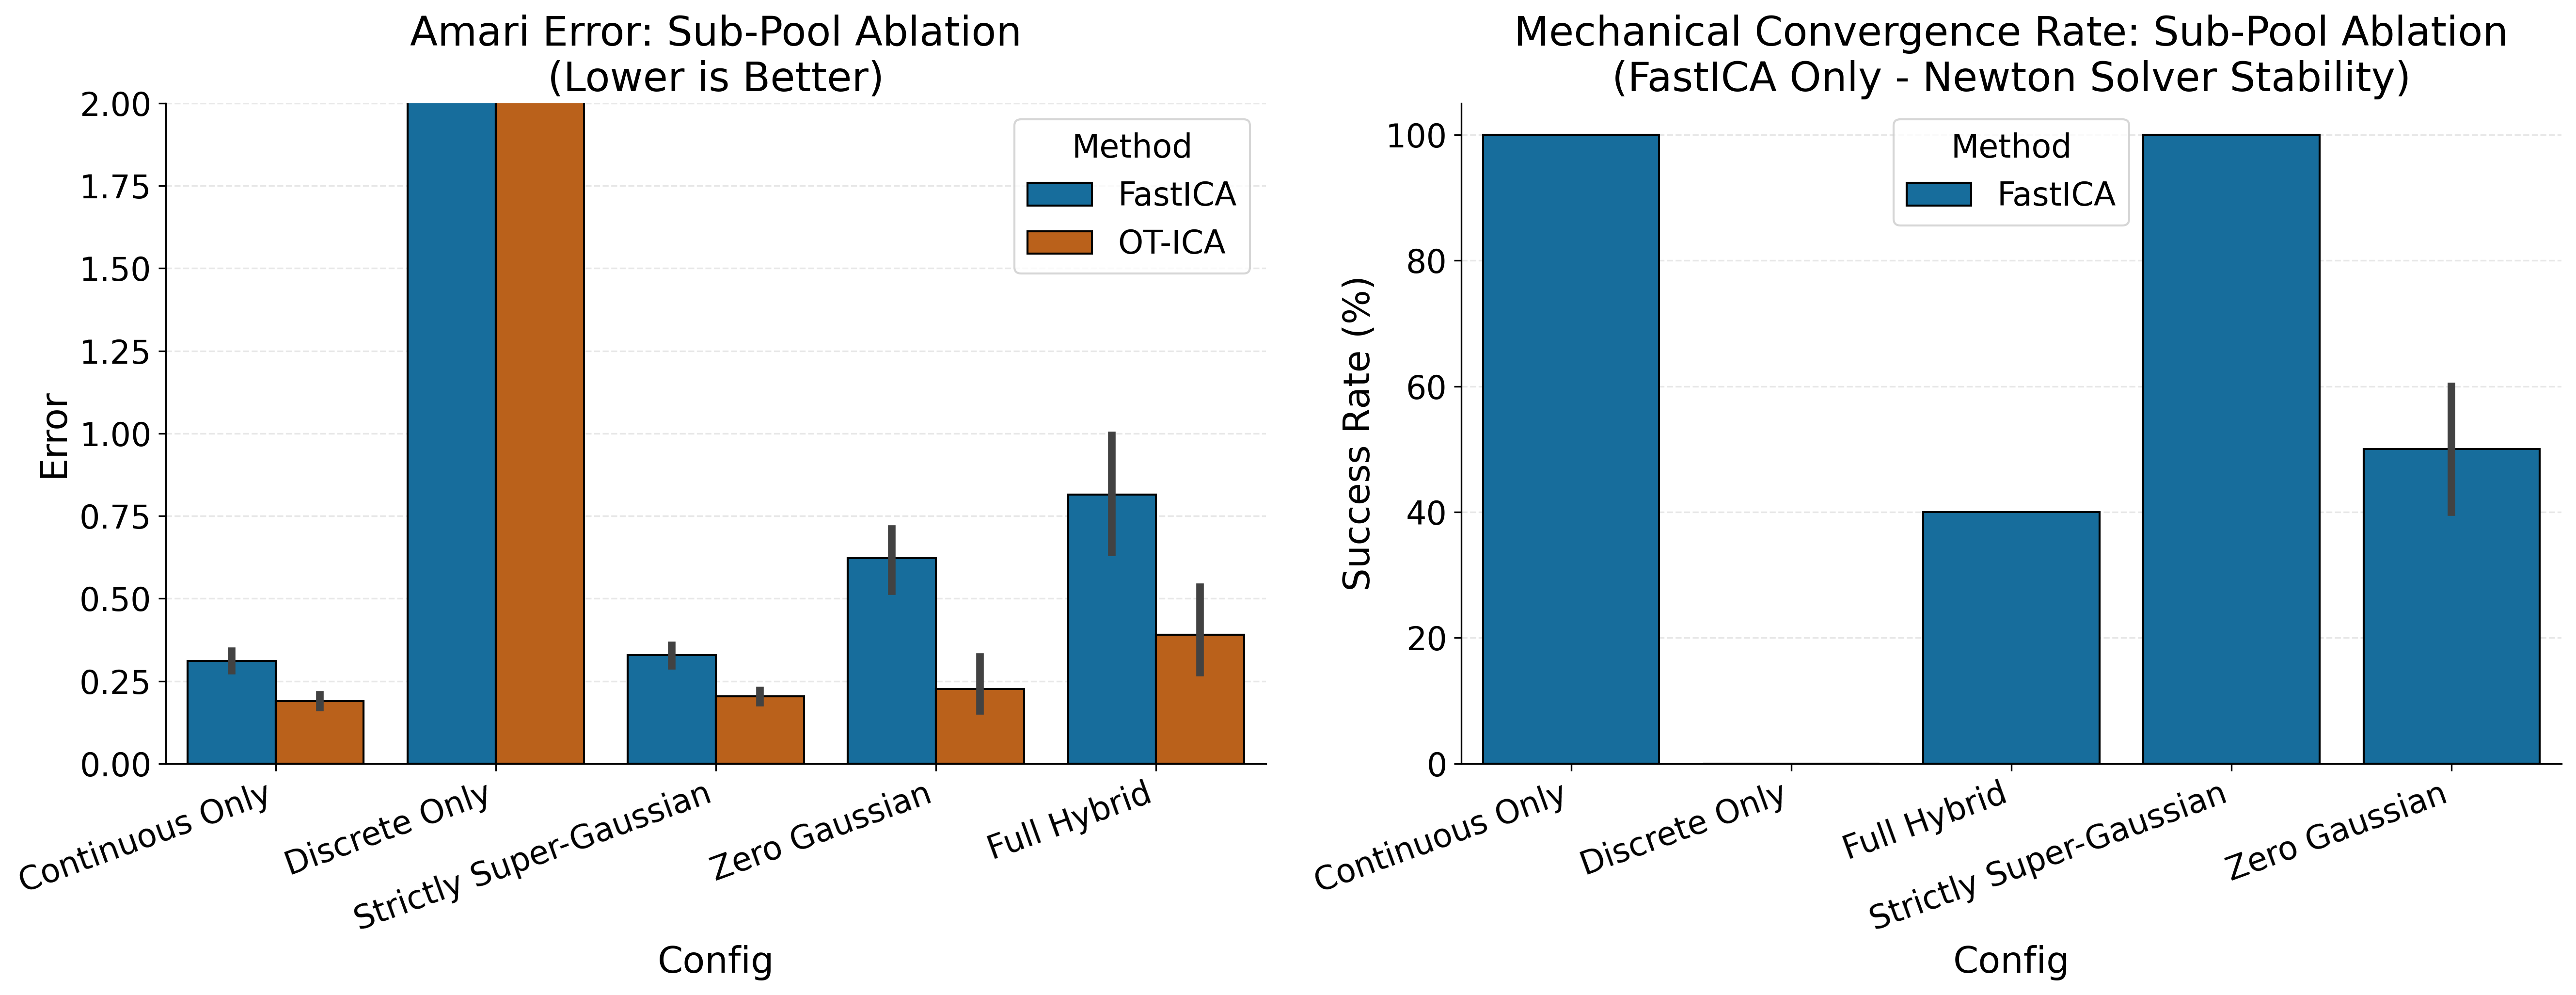
\includegraphics[width=1.0\textwidth]{general_hybrid_test.png} 
    \caption[General Hybrid Mixture Stress Test]{Amari error comparison for the Generalized Hybrid Mixture. 
    FastICA exhibits erratic behavior and high mean error, signaling a failure of its underlying curvature assumptions. 
    OT-ICA maintains stability across the tested dimensions, successfully navigating the complex non-convex landscape.}
    \label{fig:hybrid_mixture_results}
\end{figure}

In contrast, FastICA's performance is characterized by instability in the three of the five hybrid mixtures, full hybrid, zero gaussian and discrete only. 
Even at the baseline of $d=30$, FastICA consistently triggered non-convergence warnings. Crucially, providing FastICA with an extendend $10,000$ 
iteration limit did not help improve performance; the Amari error remained high ($E>0.5$). 

This confirms our hypothesis: FastICA's failure in hybrid environments is structural. When the Newton-Raphson solver is forced to 
simultaneously evaluate super gaussian signals (e.g., Laplace) and sub gaussian signals (e.g., Uniform), the fixed-point update steps 
generate contradictory gradient information. The solver is trapped in a state of permanent structural oscillation, 
perpetually overshooting the optimal projection because the uniform curvature assumed by the Newton step does not exist. 
Conversely, OT-ICA's first-order global CDF matching bypasses these local curvature traps for all but discrete only mixtures, we explore this
conundrum in the following section.

\section{Discrete Only Mixtures: A Unique Challenge}
To further understand the behavior of these algorithms in discrete environments, we isolated specific discrete distributions 
from the discrete only mixtures to observe their individual impact on the optimization landscape. 
We generated mixtures containing one continuous Gaussian source and $(d-1)$ sources of a \textit{single} discrete type (Bernoulli, Poisson, or Binomial).

\subsection{Empirical Results: Discrete Only Mixtures}
The empirical results, visualized in Figure \ref{fig:discrete_isolation}, reveal an identical performance dichotomy for both algorithms. 
While FastICA and OT-ICA proved highly capable of separating purely binary Bernoulli mixtures, both frameworks report high Amari errors ($E > 1.0$) 
when faced with the multi-step, count-based geometries of standard Poisson ($\lambda=3$) and Binomial ($n=10$) distributions. 
This shared vulnerability raises a critical question: is this breakdown caused by the fundamental geometric intractability of a 
jagged discrete optimization landscape, or do these specific parameterizations simply lack sufficient statistical non-Gaussianity 
to successfully drive blind source separation?

\begin{figure}[tbp]
    \centering
    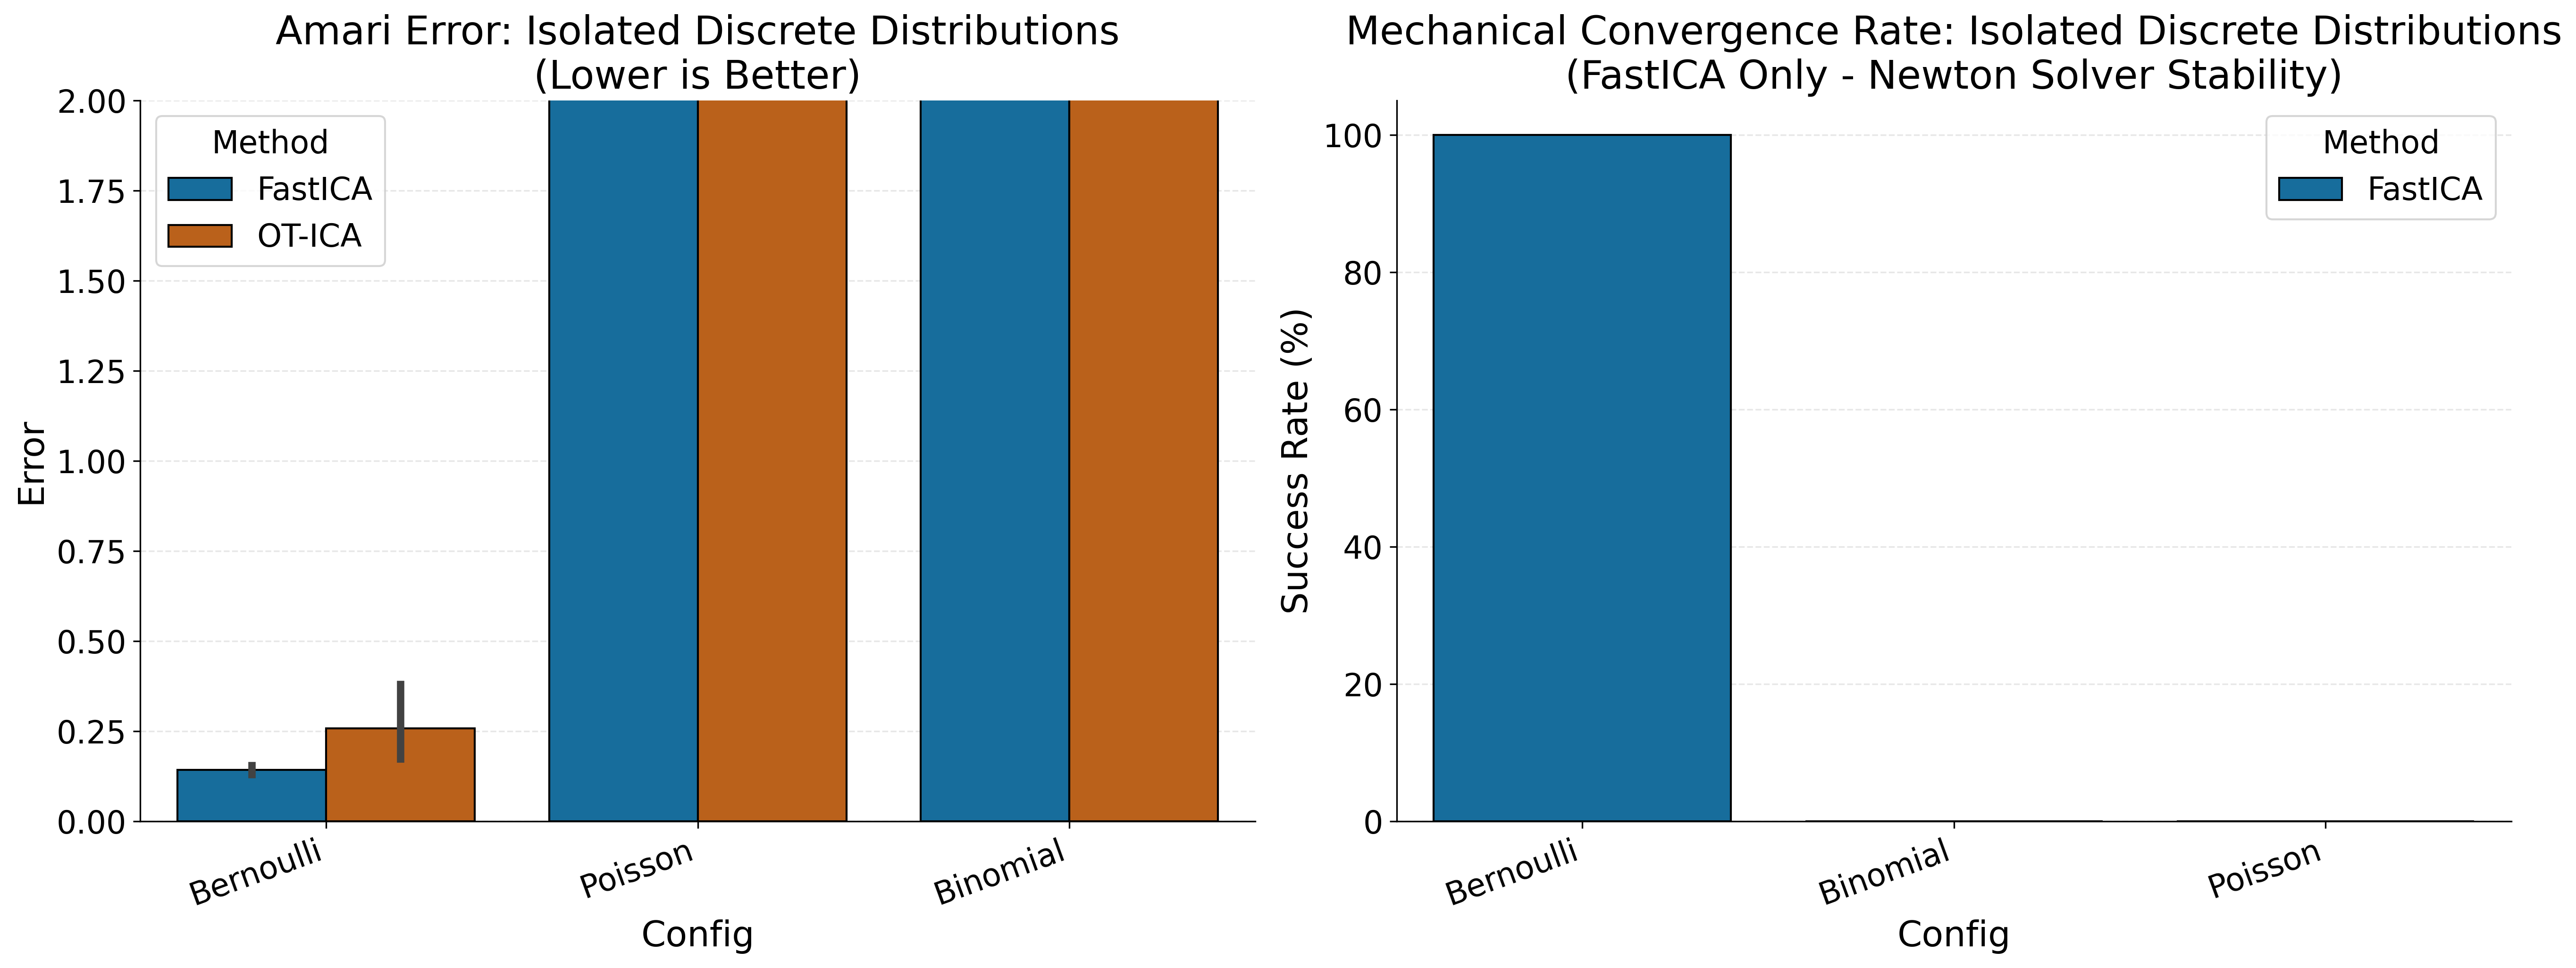
\includegraphics[width=1.0\textwidth]{isolated_discrete_test.png} 
    \caption[Performance on Isolated Discrete Pools]{Amari error and convergence rates for mixtures composed entirely of a single discrete distribution type. 
    Both FastICA and OT-ICA succeed on binary (Bernoulli) data but experience complete failure on multi-step count data (Poisson, Binomial).}
    \label{fig:discrete_isolation}
\end{figure}

%Note that convergence rates are only reported for FastICA. Because FastICA utilizes a second-order Newton solver, 
%it is susceptible to mechanical non-convergence (infinite oscillation) when assumptions are violated. 
%Conversely, OT-ICA relies on first-order L-BFGS gradient descent, which mechanically guarantees convergence to a minimum. 
%For OT-ICA, algorithmic failure manifests not as a non-convergence warning, but as convergence to a spurious local minimum, 
%which is fully captured by the Amari Error metric.

\subsection{Optimization Intractability Or Statistical Non-Gaussianity}
To determine whether the shared failure on Poisson and Binomial distributions was due to a lack of statistical non-Gaussianity 
(i.e., the distributions appearing too 'Gaussian-like') or due to the fundamental geometry of the optimization surface, 
we conducted a sensitivity analysis. We calculated the exact squared Wasserstein distance ($W_2^2$) utilized by OT-ICA, 
alongside the Logcosh proxy negentropy utilized by FastICA, to measure the distance between standard normal noise and two different parameterizations of these discrete distributions.

\begin{table}[htbp]
    \centering
    \begin{tabular}{lcc}
        \toprule
        \textbf{Distribution} & \textbf{$W_2^2$ Distance} & \textbf{Logcosh Proxy Negentropy} \\
        \midrule
        Laplace (Continuous Baseline) & 0.0398 & 0.001214 \\
        Binomial (Standard, $n=10$) & 0.0344 & 0.000031 \\
        Poisson (Standard, $\lambda=3.0$) & 0.0513 & 0.000000 \\
        Binomial (Harsh, $n=2$) & 0.2022 & 0.000267 \\
        Poisson (Harsh, $\lambda=0.5$) & 0.3384 & 0.000085 \\
        \bottomrule
    \end{tabular}
    \caption[Non-Gaussianity Sensitivity Analysis]{Comparison of non-Gaussianity metrics. While the Optimal Transport metric ($W_2^2$) correctly identifies 
    the extreme non-Gaussianity of the 'Harsh' parameterizations, FastICA's proxy negentropy completely fails to capture it, evaluating orders of magnitude lower than the continuous baseline.}
    \label{tab:w2_sensitivity}
\end{table}

As demonstrated in Table \ref{tab:w2_sensitivity}, lowering the parameters (Poisson $\lambda=0.5$, Binomial $n=2$) forces the distributions to become drastically non-Gaussian. 
The Optimal Transport metric ($W_2^2$) perfectly captures this reality, registering distances up to nearly ten times further from the Gaussian baseline than the Laplace distribution, 
which both algorithms easily separated in earlier tests. However, while the actual data is highly non-Gaussian, FastICA's negentropy approximation (\textit{logcosh}) 
becomes mathematically indifferent to the discrete count data. Even on the highly non gaussian 'Harsh' parameterizations, the proxy negentropy evaluates to values on 
order of magnitude lower than the continuous Laplace baseline, and evaluates to effectively zero for the Standard Poisson. 

This establishes a critical divergence in the root cause of failure on discrete data for FastICA and OT-ICA. FastICA's failure on these distributions is inherently statistical; 
its proxy objective function is structurally indifferent to the non-Gaussianity of sparse discrete data. Conversely, OT-ICA's metric perfectly measures the true non-Gaussianity, 
proving that its corresponding failure on these same distributions must be dictated entirely by the intractability of the optimization landscape itself.

To visually confirm why both algorithms struggle with these distributions under different conditions, we mapped the 1D optimization surfaces for both 
the $W_2^2$ distance (OT-ICA) and the \textit{logcosh} proxy (FastICA) across the standard and harsh parameterizations. 
As illustrated in Figure \ref{fig:optimization_surface}, the discrete nature of the data fundamentally fractures the loss landscape, revealing the distinct weaknesses of each algorithm. 

\begin{figure}[tbp]
    \centering
    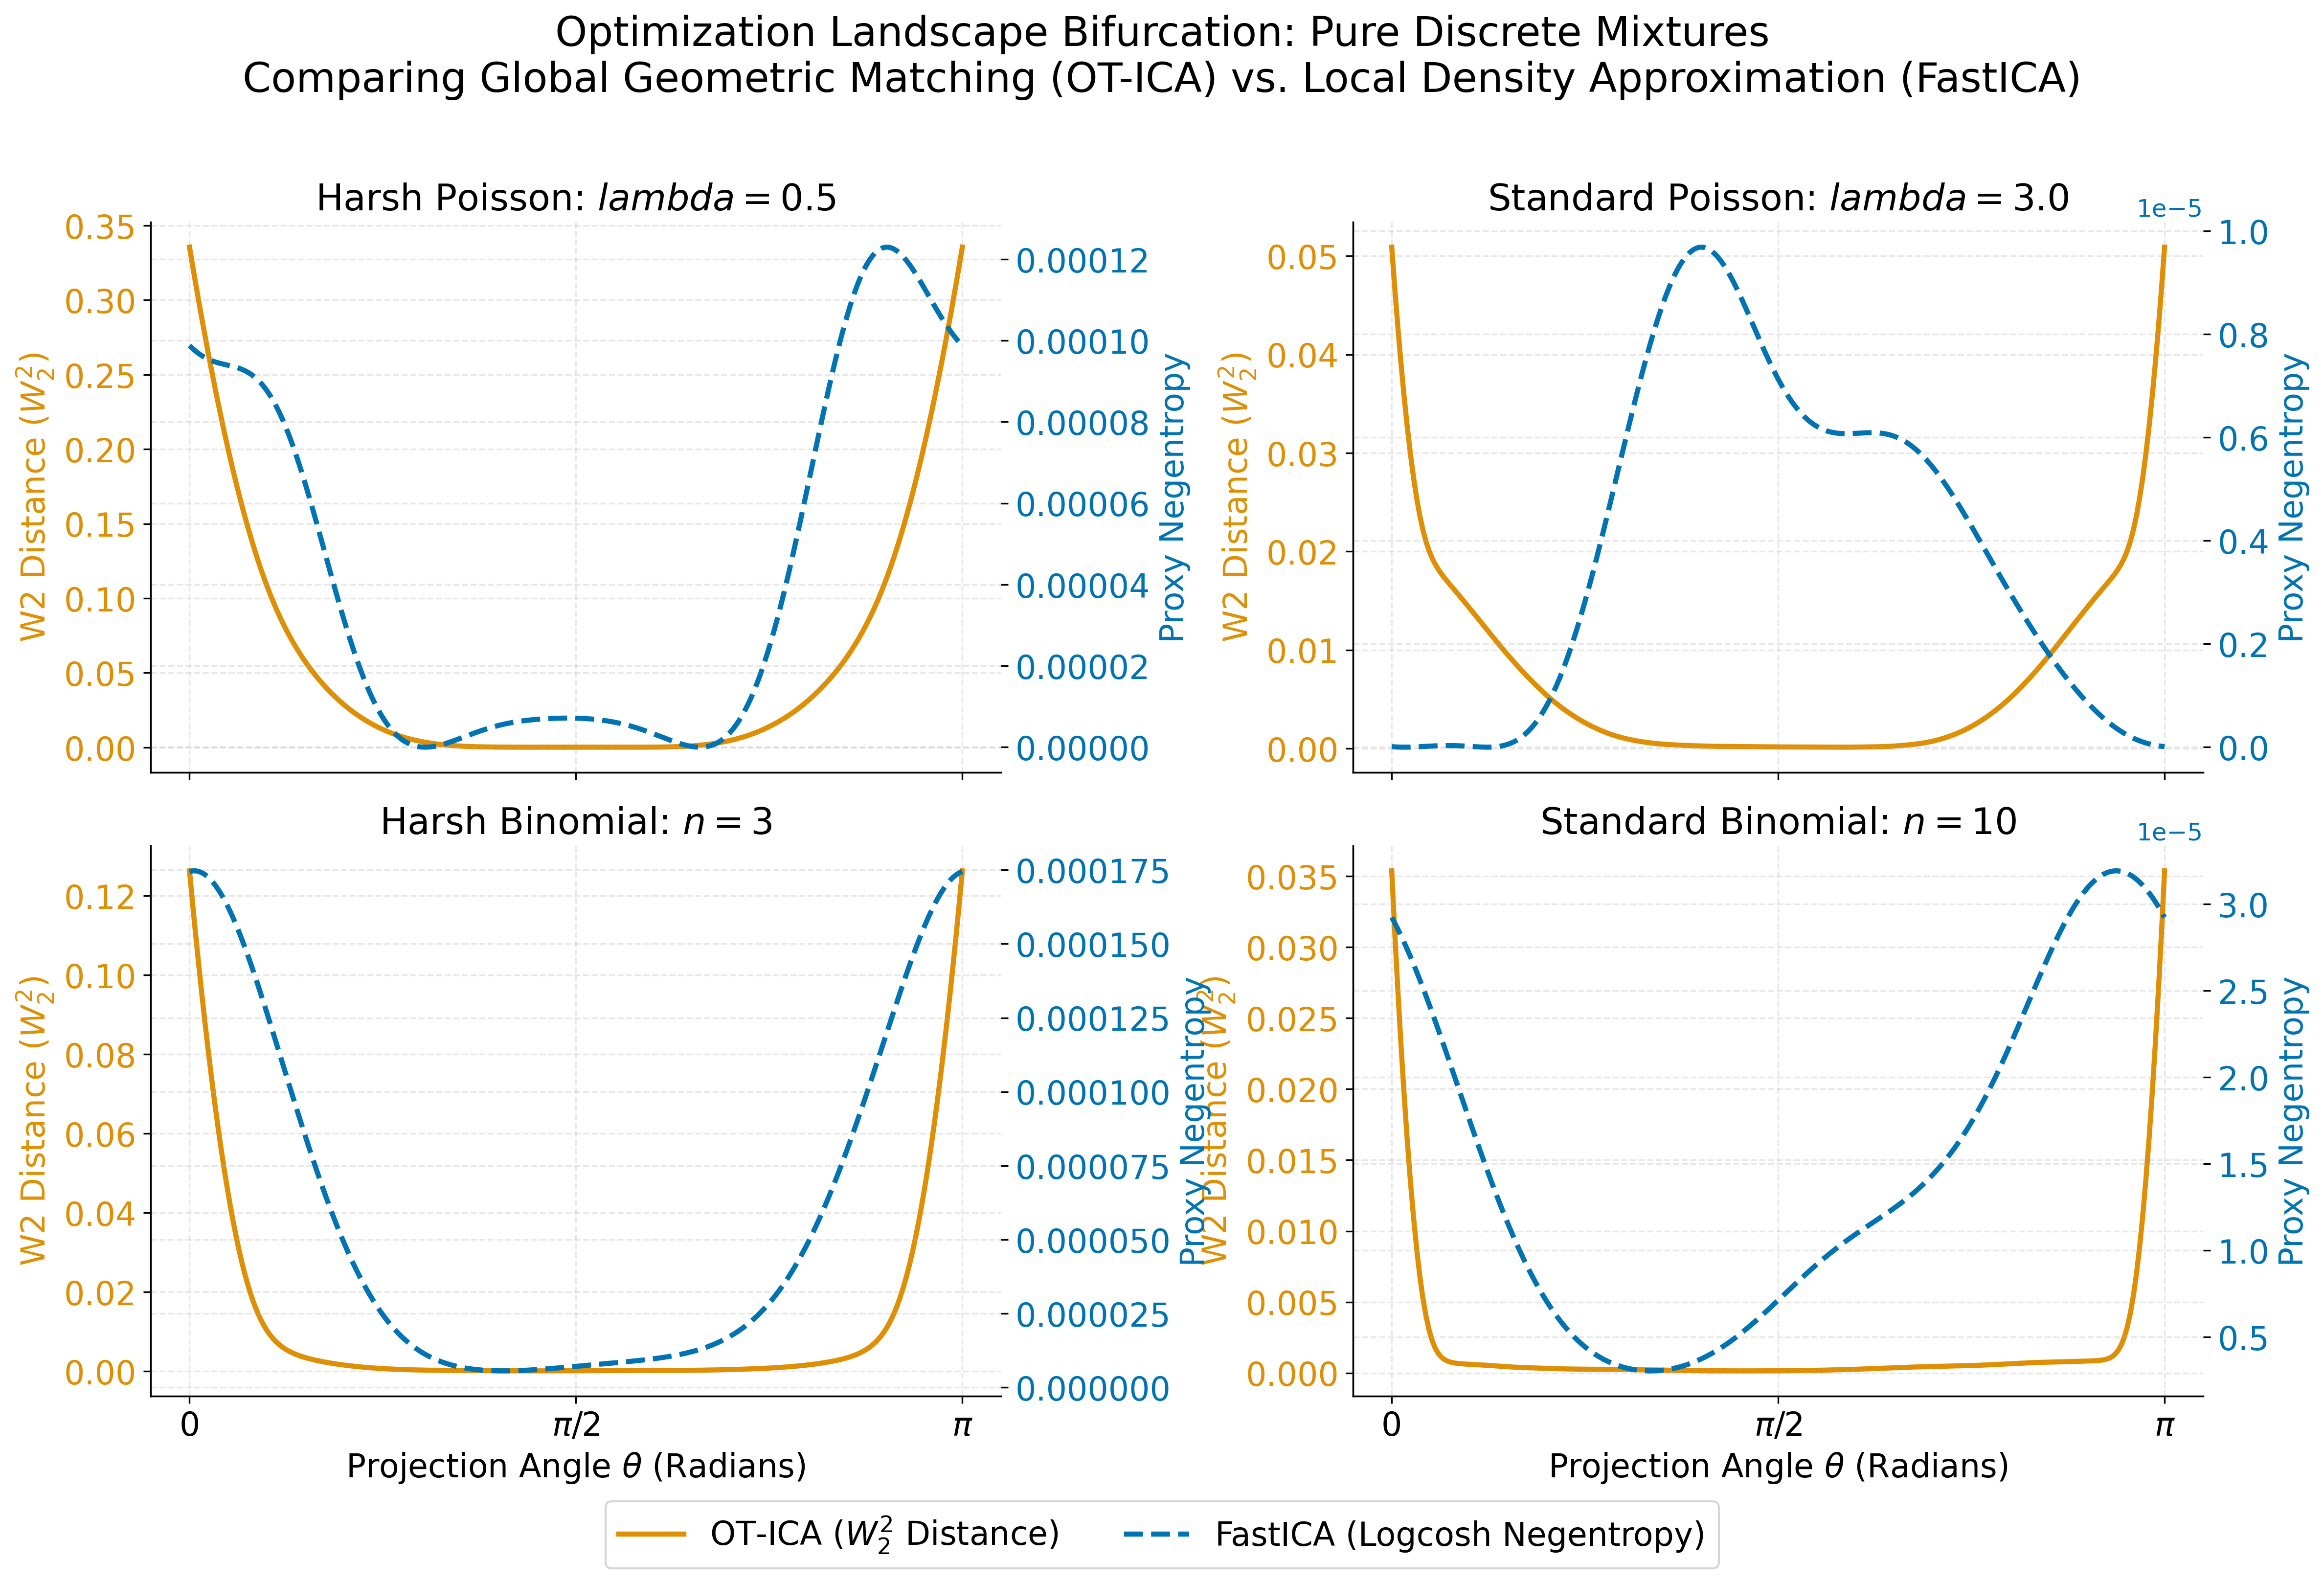
\includegraphics[width=1.0\textwidth]{all_optimization_surfaces.png}
    \caption[Optimization Surface of Discrete Mixtures]{The 1D optimization landscapes for discrete mixtures. 
    The standard parameterizations (right column) exhibit relatively smooth objectives. 
    The harsh parameterizations (left column) severely fracture the OT-ICA surface into non-convex geometric plateaus,
    while simultaneously blunting the FastICA proxy approximation to microscopic scales ($10^{-5}$).}
    \label{fig:optimization_surface}
\end{figure}

For FastICA (dashed blue line), the \textit{logcosh} proxy landscape appears to possess structural peaks, but observing the secondary y-axis reveals that 
the function has effectively flatlined at a microscopic scale ($1e-5$). Because the FastICA Newton solver divides by the second derivative, 
this lack of meaningful gradient amplitude causes the algorithmic curvature to vanish. The solver loses its convergence guarantees and thus fails.

Conversely, for OT-ICA (solid orange line), the exact geometric matching reflects the step-function nature of the discrete empirical CDF. 
While this guarantees the true global optimum is preserved, it nonetheless creates flat plateaus at the bottom of the valleys where the gradient is exactly zero. 
This creates a geometrically intractable landscape that prematurely stalls the L-BFGS gradient solver before it reaches the exact true components.

\subsection{Empirical Results: Harsh Discrete Environments}
If FastICA's failure is statistical and OT-ICA's failure is intractability of optimization, evaluating the algorithms on the 'Harsh' parameterizations should 
yield highly bifurcated results based on the shape of the specific discrete distribution. We executed a final evaluation using this parameterizations.

\begin{figure}[tbp]
    \centering
    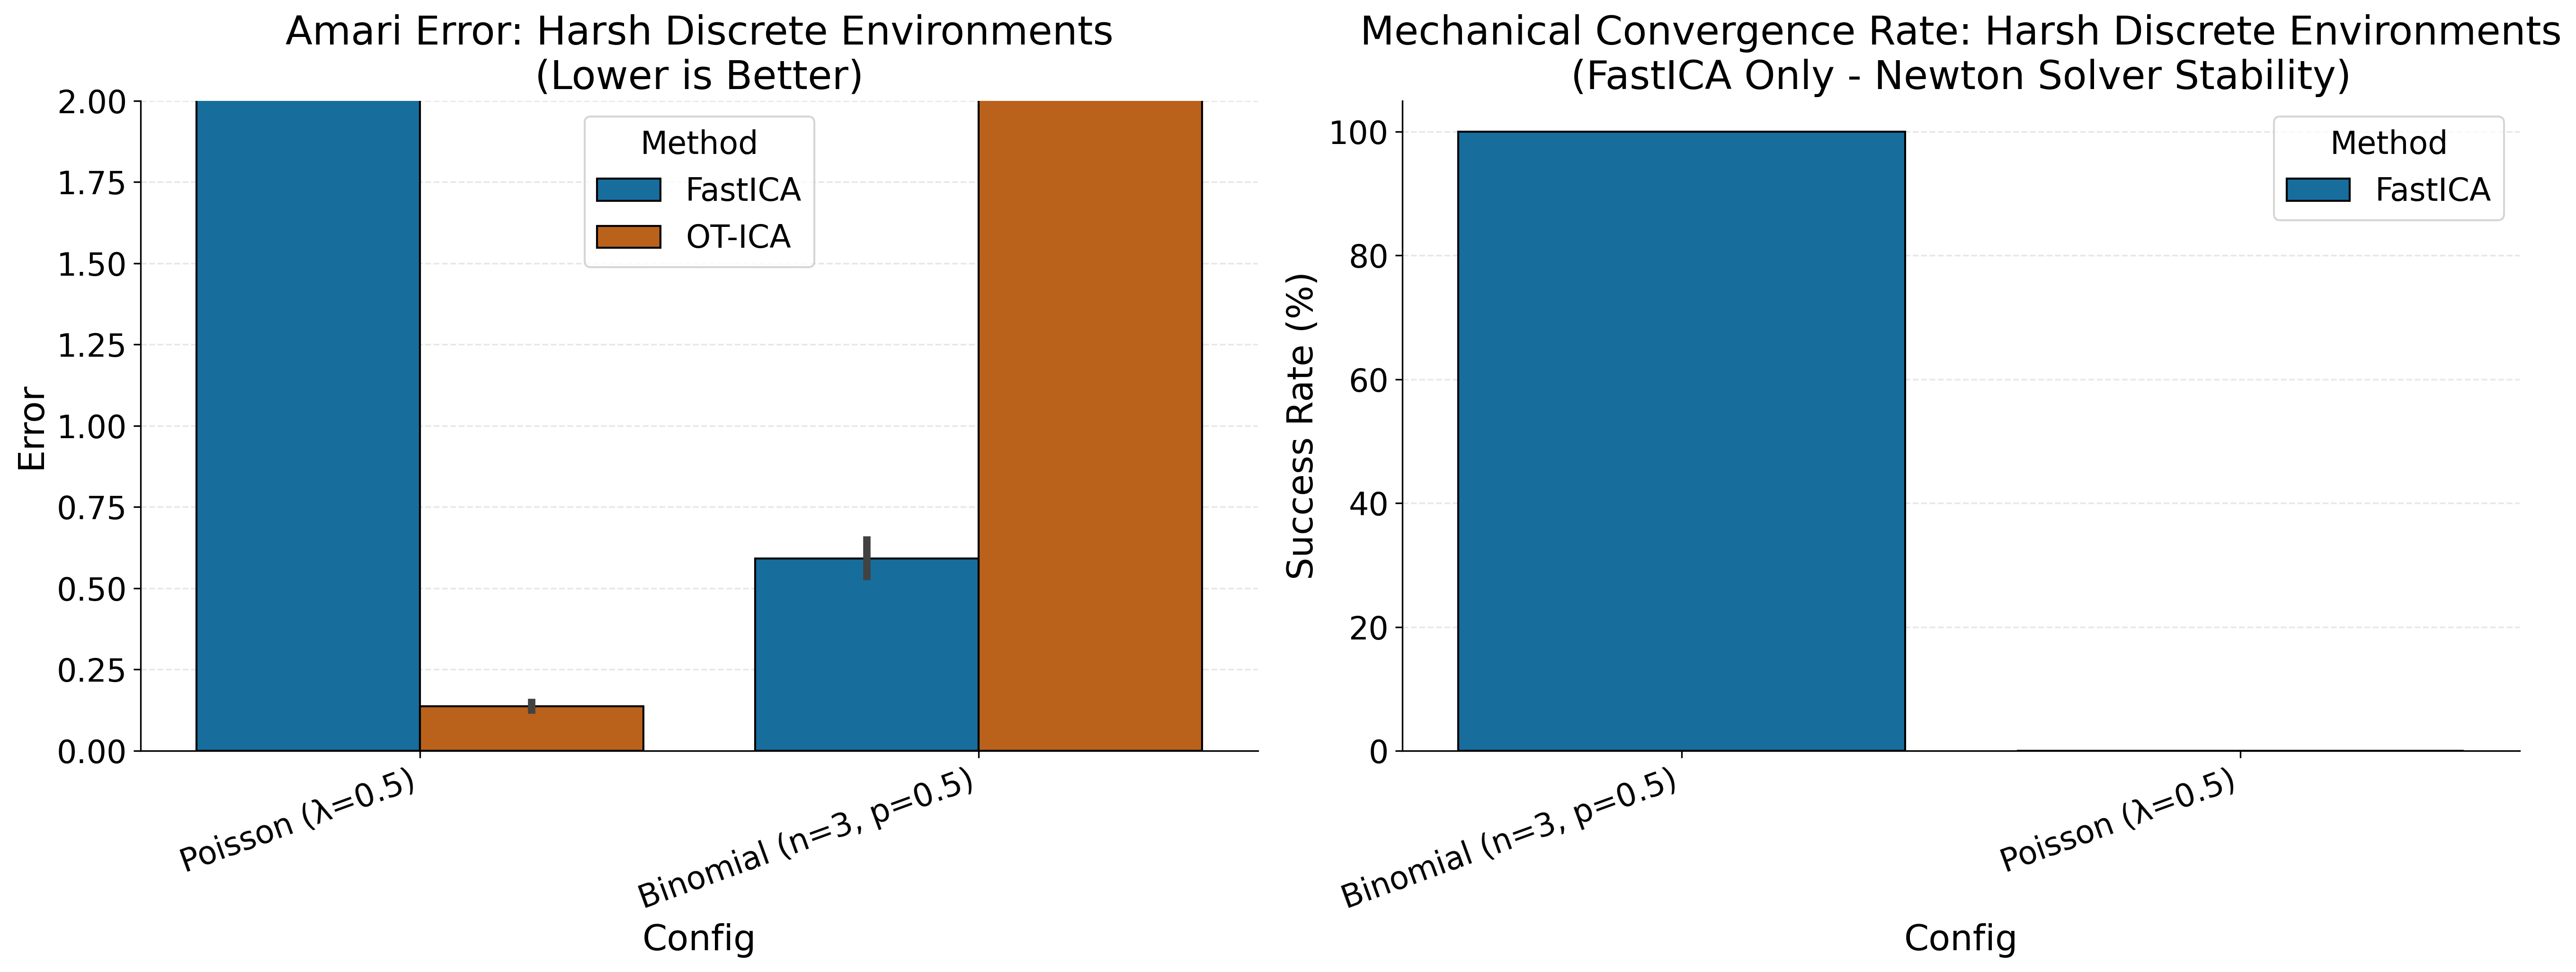
\includegraphics[width=1.0\textwidth]{binomial_poisson_fast_vs_ot_ica.png} 
    \caption[Performance on Harsh Discrete Environments]{Amari Error and FastICA Convergence for 'Harsh' discrete parameterizations. 
    FastICA suffers complete mechanical failure on the Poisson distribution, while OT-ICA's performance bifurcates based on the geometric width of the optimization plateau.}
    \label{fig:harsh_discrete}
\end{figure}

The results, shown in Figure \ref{fig:harsh_discrete}, definitively prove this divergence. For the harsh Poisson mixture ($\lambda=0.5$), 
FastICA experienced a 0\% mechanical convergence rate. The solver mathematically collapsed due to the vanished curvature observed in the optimization surface. 
Conversely, OT-ICA achieved excellent separation ($E \approx 0.15$). This success occurs because the highly skewed nature of the harsh Poisson creates a relatively narrow 
flat plateau at the minimum of the optimization surface. The gradient remains strong enough to guide the solver exceptionally close to the true independent component before 
the plateau is encountered (Figure \ref{fig:optimization_surface}). However, for the harsh Binomial mixture ($n=3$), OT-ICA fails, despite the distribution possessing a significant 
$W_2^2$ non-Gaussian gap. Unlike the skewed Poisson, the Binomial distribution remains perfectly symmetric. As seen in Figure \ref{fig:optimization_surface}, this symmetry creates a wide plateau 
at the bottom of the loss landscape. The gradient solver falls into this valley early, and the algorithm permanently stalls while still mathematically far away from 
the correct unmixing projection, resulting in a severe Amari error of $E > 2.0$.

\section{Synthesis: The Case for OT-ICA}
The empirical evaluations throughout this chapter reveal a critical distinction between the theoretical identifiability of ICA and the mechanical realities of optimization. 
While statistical non-Gaussianity guarantees that independent sources can be theoretically separated, extracting them via Optimal Transport requires a geometrically tractable optimization surface. As observed in the pure discrete environments, jagged step-functions create flat, zero-gradient plateaus that can trap first-order solvers, despite the objective function correctly identifying the non-Gaussianity.

This optimization bottleneck highlights precisely why OT-ICA thrives in generalized, heterogeneous environments. As demonstrated in Figure \ref{fig:hybrid_mixture_results}, 
OT-ICA successfully disentangled 'Full Hybrid' mixtures combining both continuous and discrete variables. In these mixed environments, the continuous distributions act as a mathematical smoothers; 
they smooth the overall joint Cumulative Distribution Function (CDF), effectively bridging the discrete geometric gaps and eliminating the zero-gradient plateaus. 
This smoothing allows the gradient solver to successfully leverage the global Optimal Transport metric across the entire manifold.

Crucially, this hybrid environment exposes the fundamental divergence in reliability between the two algorithms. FastICA relies on static, 
local negentropy approximations (\textit{logcosh}). As demonstrated throughout this chapter, these approximations create rigid mathematical blind spots, specifically 
the zero-negentropy trap and vanishing algorithmic curvature. When forced to navigate a generalized hybrid mixture containing contradictory statistical structures, 
FastICA's proxy is imprecise, causing the Newton solver to fail.

By contrast, because OT-ICA explicitly maps the full empirical geometry of the data, it is inherently immune to these local proxy blind spots. 
While OT-ICA experiences performance degradation in highly complex or purely symmetric discrete environments, these are strictly optimization landscape issues stemming from 
the non-convexity of the Stiefel manifold. Because OT-ICA's global metric remains mathematically valid across all non-Gaussian domains, its performance scales directly with compute power. 
When provided with dense parallel restarts or higher computational precision, OT-ICA demonstrably navigates these complex landscapes and restores accurate separation in 
regimes where FastICA permanently stalls.

Ultimately, FastICA retains a massive advantage in computational efficiency, making it the strictly superior choice for homogeneous mixtures of standard, 
well-behaved continuous distributions where its convergence is practically instantaneous. However, real-world data is rarely pristine. 
In heterogeneous, hybrid environments where structural assumptions are routinely violated, computational speed becomes irrelevant if the algorithm fundamentally cannot converge. 
By trading temporal efficiency for global geometric awareness, OT-ICA provides a robust alternative capable of disentangling complex mixtures where traditional proxies fail.

\section{Application: Price Discovery and Information Shares}

\subsection{Non-Gaussianity in Econometric Market Microstructure}
To demonstrate the empirical utility of the OT-ICA framework, we apply it to the problem of price discovery in financial econometrics. 
In fragmented financial markets where the same asset is traded across multiple venues, 
determining which market contributes most to the incorporation of new information (price discovery) is a non-trivial challenge. 
Standard vector error correction models (VECMs) identify information shares by relying on the uncorrelation of price innovations. 
However, as demonstrated by Zema and Cordoni \citeyear{zema2025}, any identification approach relying solely on uncorrelation is statistically equivalent up to an orthogonal transformation. 

By leveraging the inherent non-Gaussianity of latent market shocks, ICA can be utilized to resolve this orthogonal ambiguity, 
unifying disparate price discovery metrics into a single, unique measurement of market information shares. 

\subsection{Economic Identification Strategy}
While ICA successfully identifies the independent structural shocks driving the market, the raw statistical output remains subject to the inherent permutation and sign ambiguities 
discussed in Chapter 2. To translate these statistical components into meaningful economic drivers, we impose two strict economic identification constraints.

First, to resolve the permutation ambiguity, we enforce a Dominant Diagonal constraint. 
We postulate that the structural shock assigned to Market $i$ must be the specific shock that contributes the maximum variance to that market's price innovations. 
We implement this assignment algorithmically using the Hungarian Algorithm, which uniquely solves the optimal bipartite matching problem between the recovered independent components 
and the individual markets.

Second, to resolve the sign ambiguity, we enforce a Positive Impact constraint based on the economic theory of positive spillovers. 
We assert that a structural innovation representing 'good news' must have a positive initial impact on its own market price. 
Any column of the unmixing matrix that violates this economic logic is sign-flipped, ensuring the final structural parameters are economically interpretable. 

\subsection{Empirical Results on Simulated Market Data}
To validate the efficacy of our Optimal Transport based identification strategy, we simulated a fragmented market scenario. 
The simulation targets three distinct markets with pre-defined theoretical Information Shares of $12\%$, $24\%$, and $64\%$, respectively. 
The market innovations were generated using heavy-tailed Student-t distributions to satisfy the fundamental non-Gaussianity requirements of the ICA framework. 
We executed 500 Monte Carlo simulations, each comprising 5,000 observations.

For each simulation, the OT-ICA framework successfully recovered the independent structural shocks. Figure \ref{fig:shock_recovery} illustrates a representative run, 
demonstrating the high correlation between the true generative shocks and the empirical shocks estimated by OT-ICA. The tight alignment along the identity line confirms that 
the algorithm successfully unmixed the latent variables prior to any economic transformation.

\begin{figure}[tbp]
    \centering
    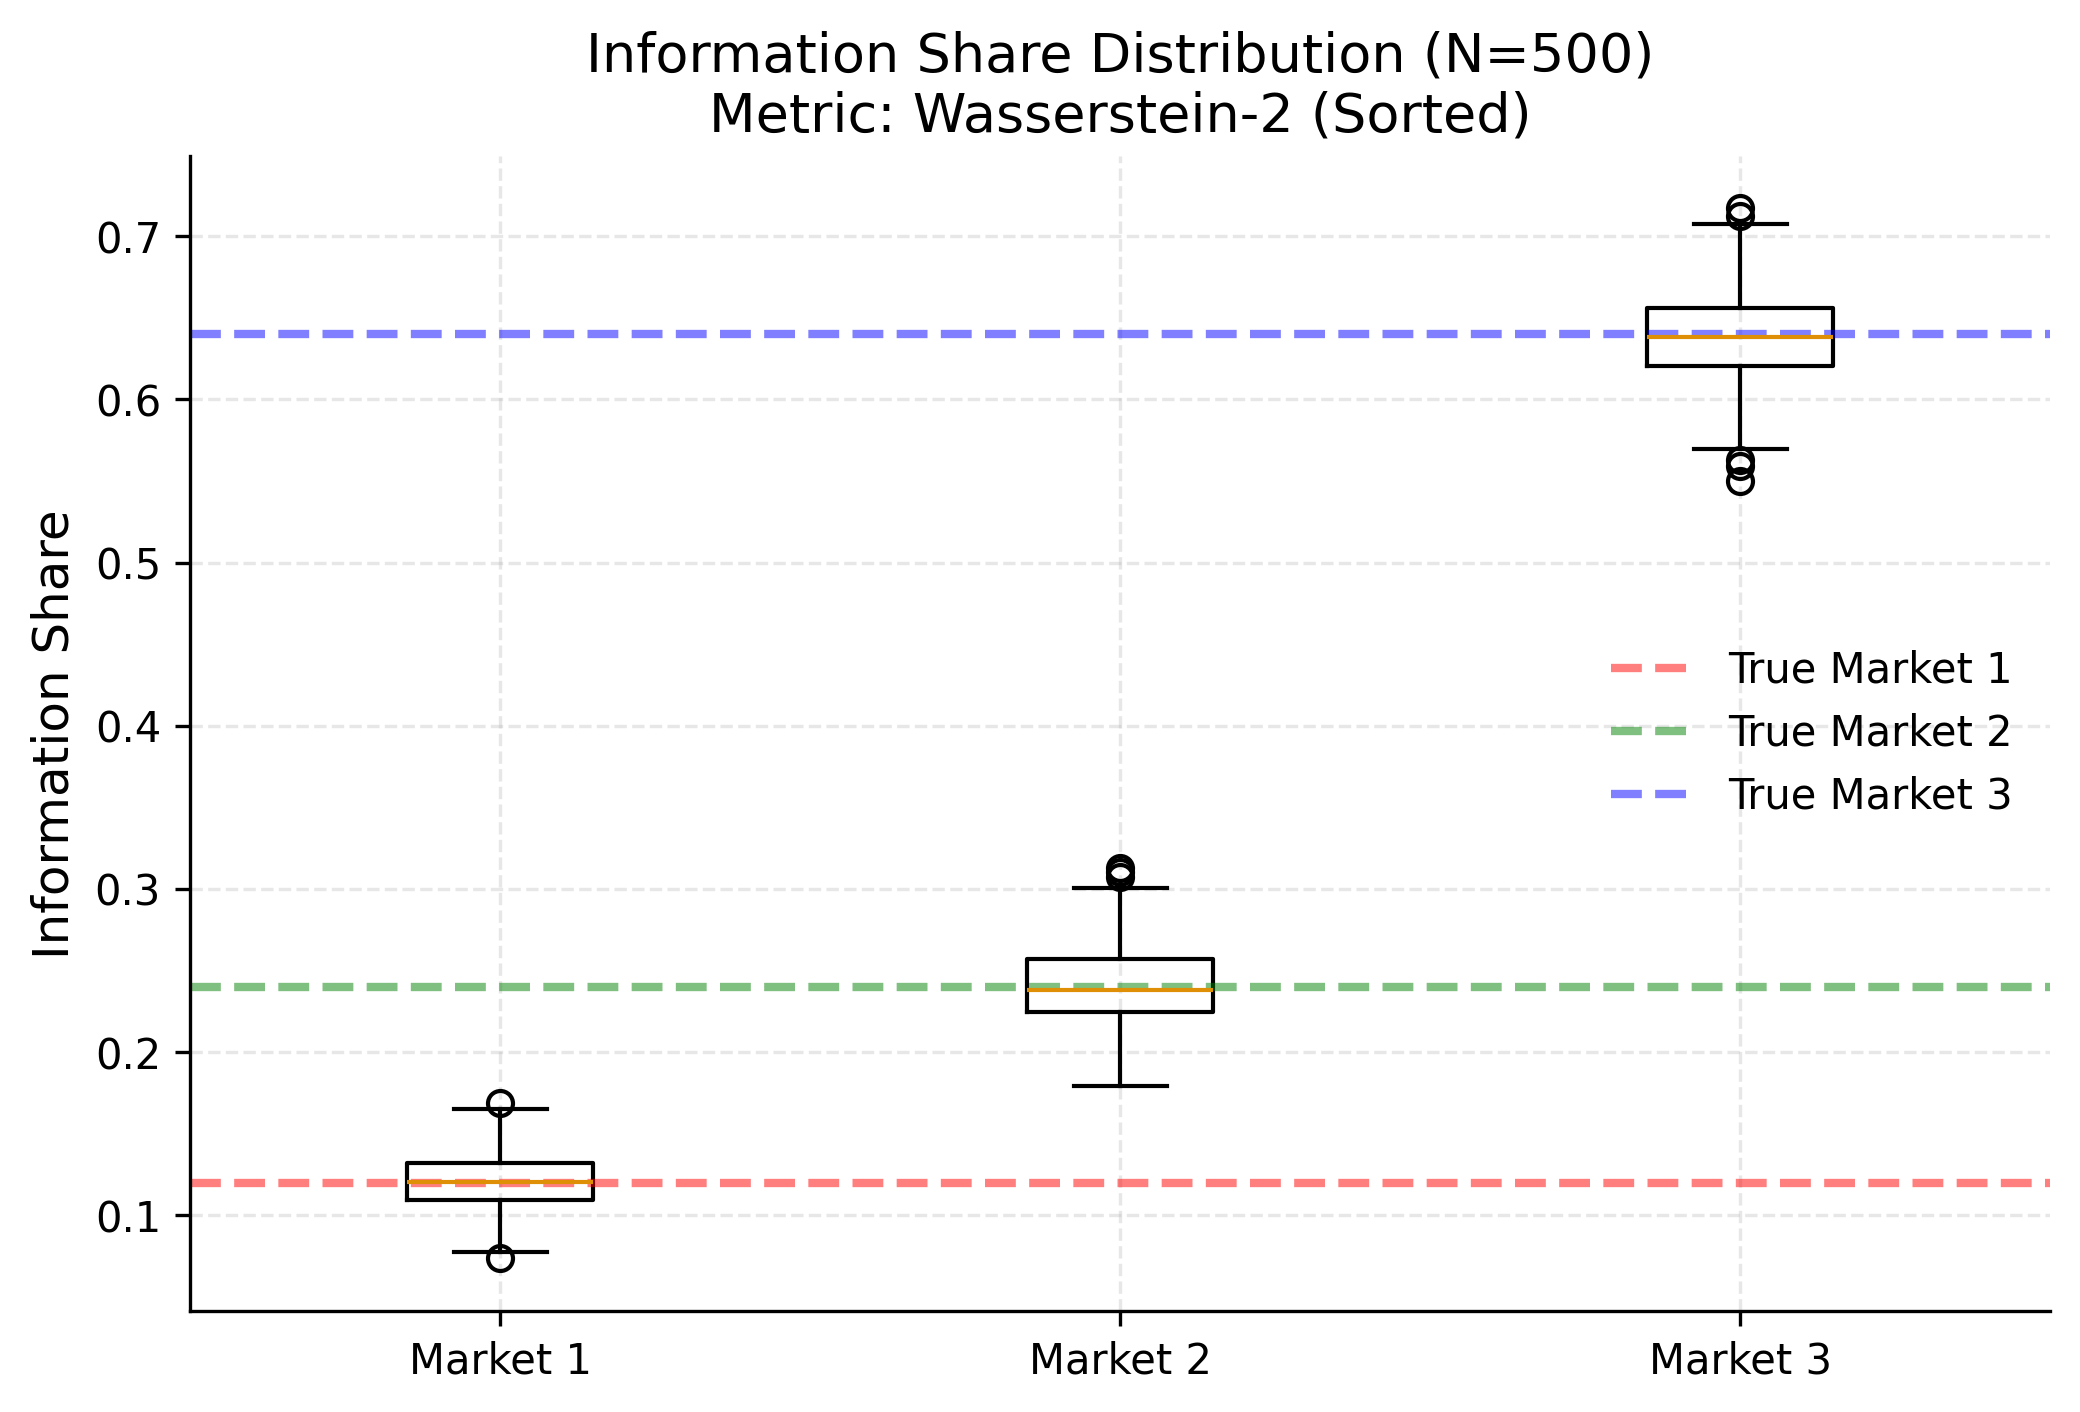
\includegraphics[width=1.0\textwidth]{shock_recovery_scatter.png}
    \caption[Recovery of Structural Shocks via OT-ICA]{Pairplot demonstrating the recovery of true structural shocks versus the estimated shocks from OT-ICA 
    for a single Monte Carlo run. \textbf{Takeaway:} The strong linear alignment indicates highly accurate unmixing of the latent non-Gaussian market innovations.}
    \label{fig:shock_recovery}
\end{figure}

By applying the economic identification constraints detailed in the previous section, specifically, the Dominant Diagonal and Positive Impact rules, 
we uniquely mapped these statistical components to their corresponding markets and calculated the resulting empirical information shares.

Table \ref{tab:simulated_is_results} presents the aggregate results across all 500 simulations. The OT-ICA estimator, combined with our economic identification strategy, 
demonstrates exceptional accuracy. The mean estimated information shares converge almost exactly to their theoretical targets, with minimal standard deviations indicating 
a highly stable recovery process. 

\begin{table}[htbp]
    \centering
    \begin{tabular}{@{}lccc@{}}
        \toprule
        \textbf{Market / Source} & \textbf{True IS} & \textbf{Estimated IS (Mean)} & \textbf{Standard Deviation} \\
        \midrule
        Market 1 & 0.1200 & 0.1212 & 0.0161 \\
        \addlinespace
        Market 2 & 0.2400 & 0.2399 & 0.0245 \\
        \addlinespace
        Market 3 & 0.6400 & 0.6389 & 0.0260 \\
        \bottomrule
    \end{tabular}
    \caption[Simulation Results for Information Share Recovery]{Monte Carlo simulation results comparing true Information Shares (IS) against the estimated IS recovered 
    via the OT-ICA framework over 500 runs. \textbf{Takeaway:} OT-ICA robustly and accurately recovers the true structural parameters of the market.}
    \label{tab:simulated_is_results}
\end{table}

Furthermore, Figure \ref{fig:is_distribution} illustrates the empirical density of the estimated information shares across all simulation runs. 
The distributions are tightly centered around the true parameter values, empirically confirming that OT-ICA effectively resolves the orthogonal ambiguity and robustly recovers 
the structural drivers of price discovery.

\begin{figure}[tbp]
    \centering
    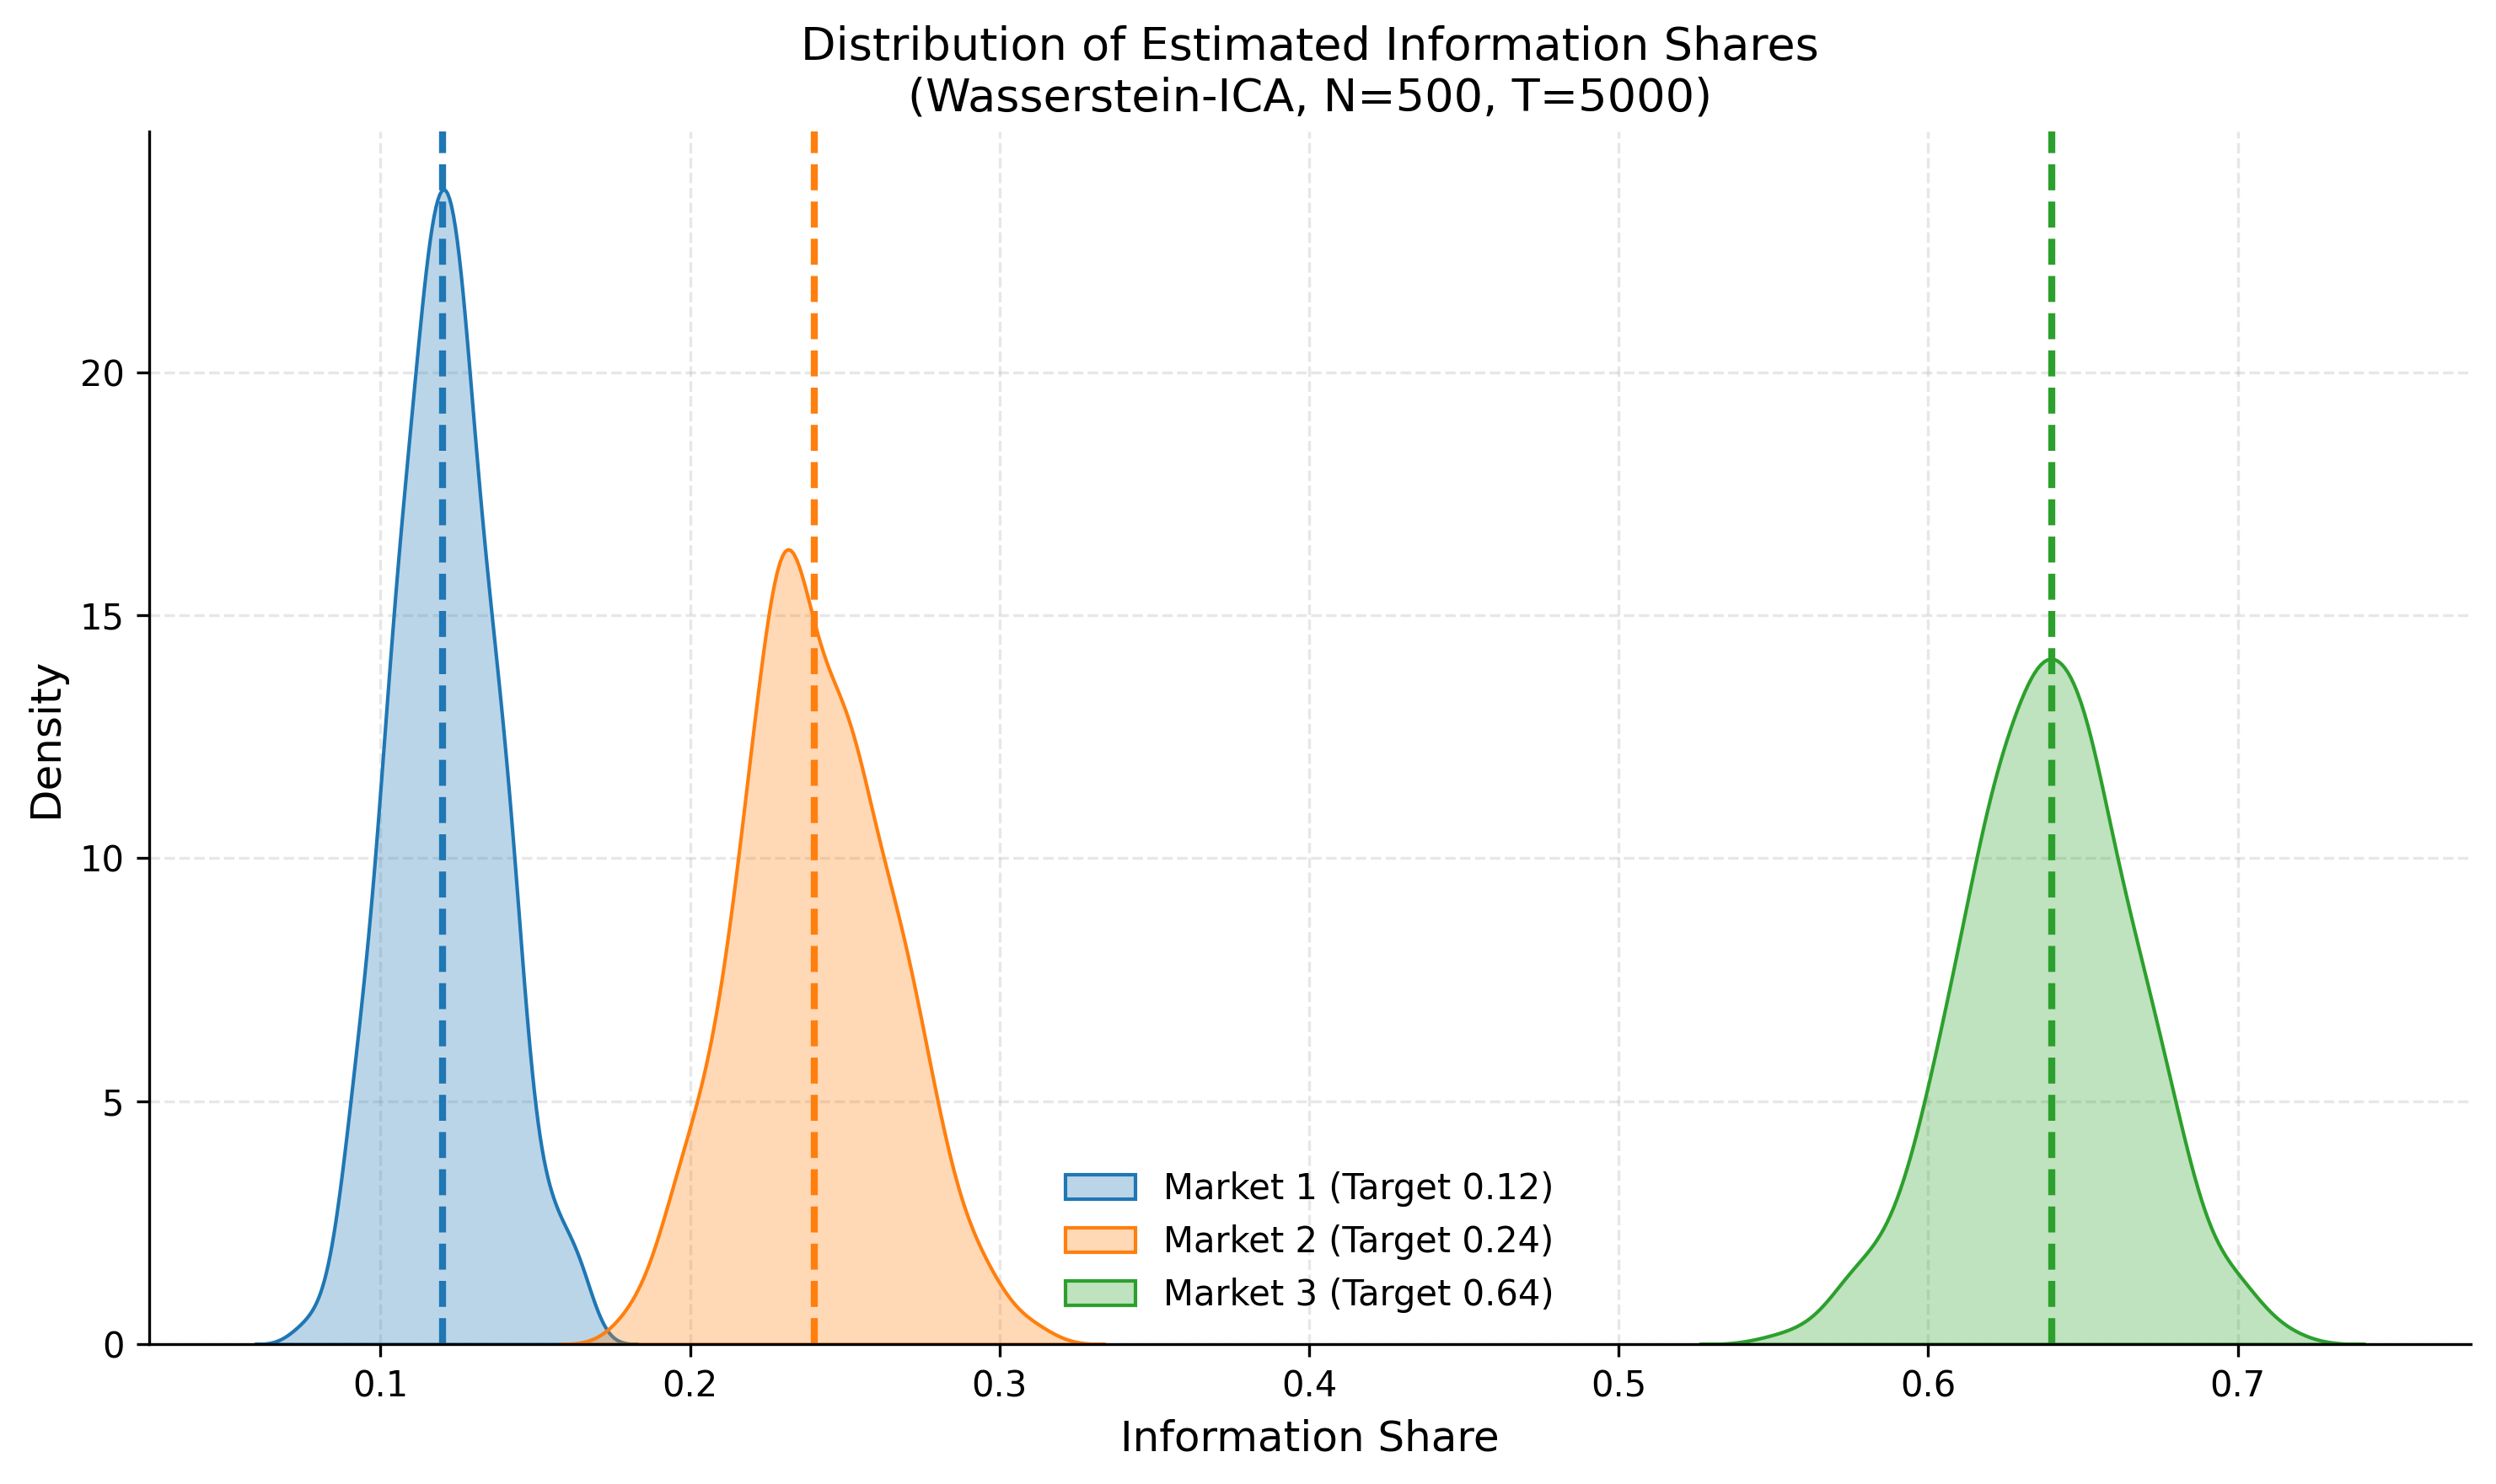
\includegraphics[width=1.0\textwidth]{econ_applicatn_is_distribution.png} 
    \caption[Empirical Distribution of Estimated Information Shares]{Empirical density distributions of the estimated Information Shares across 500 Monte Carlo simulations. 
    The vertical dashed lines represent the true theoretical values. \textbf{Takeaway:} The tight, unimodal centering around the true values demonstrates 
    the lack of structural oscillation in the Optimal Transport gradients.}
    \label{fig:is_distribution}
\end{figure}


% -----------------------------------------------------------------
% CHAPTER 6: CONCLUSION
% -----------------------------------------------------------------
\chapter{Conclusion}

\section{Summary of Contributions}
This thesis proposed and rigorously evaluated the Optimal Transport Independent Component Analysis (OT-ICA) framework, shifting the paradigm of linear source separation 
from local proxy approximations to global geometric matching. By formulating the search for independent components as a minimization of the squared Wasserstein distance ($W_2^2$) 
to a standard normal distribution on the Stiefel manifold, we addressed critical mathematical vulnerabilities inherent in proxy algorithms like FastICA.

Our theoretical analysis established that the squared Wasserstein distance strictly bounds mixture non-Gaussianity, providing a mathematically sound objective for extracting latent sources. 
Empirically, we demonstrated that while algorithms like FastICA fail in the presence of specific structural blind spots, such as zero-negentropy topologies 
and vanishing curvature, OT-ICA consistently maintains algorithmic stability. By mapping the full cumulative distribution function rather than relying on point-estimates of density, 
OT-ICA proved uniquely capable of resolving highly complex, generalized hybrid mixtures where proxy solvers infinitely oscillate.

Furthermore, we introduced several critical algorithmic enhancements to make optimal transport computationally viable for ICA. These included the derivation of exact analytical Gaussian 
targets to eliminate discretization noise, batched vectorization for parallel hypothesis exploration, and the novel application of Gaussian dithering to prevent 
the piecewise linear shattering of discrete optimization landscapes. Finally, we demonstrated the practical utility of this framework in a financial econometrics setting, 
utilizing the robust non-Gaussian recovery of OT-ICA to uniquely resolve orthogonal ambiguities in market price discovery. Ultimately, this framework establishes a new baseline for handling structurally heterogeneous data across the broader fields of signal processing and machine learning.

\section{Limitations}
Despite its geometric robustness, the OT-ICA framework is subject to specific constraints that delineate its operational boundaries. 
The primary limitation is computational efficiency. Because the exact Hessian of the Wasserstein distance requires continuous density estimation, 
OT-ICA cannot leverage the quadratic or cubic convergence guarantees of FastICA's fixed-point iteration. Instead, the framework relies on first-order 
Quasi-Newton methods (L-BFGS) combined with dense parallel random restarts to navigate the non-convex objective. This results in a significant temporal overhead, 
where the execution time scales exponentially with the dimensionality of the search space.

Furthermore, the framework encounters a strict statistical performance ceiling dictated by the curse of dimensionality. While 1D Optimal Transport is statistically robust, 
the global search for the unmixing matrix is bound by the statistical resolution of the joint distribution. As the dimensionality expands, 
the non-convex search space of the orthogonal group $O(d)$ becomes increasingly complex. The 'volume' of the search space increases, and the $\mathcal{O}(N \log N)$ sorting cost is compounded by the necessity for $K$ restarts to avoid local minima. 
In our empirical evaluations, a fixed sample size of $N=10,000$ became insufficient for $d > 40$, as the surface area of the manifold became too vast for stable recovery, 
matching the statistical limits of linear ICA with respect to Amari Error.

Finally, there remains a geometric bottleneck regarding purely discrete distributions. While Gaussian dithering successfully smooths step-wise empirical CDFs, 
purely symmetric and sparse discrete distributions (such as a low-$n$ Binomial distribution) still yield intractable optimization landscapes with zero-gradient plateaus. 
While OT-ICA excels in hybrid environments where continuous variables act as mathematical smoothers, isolating purely discrete, symmetrically clustered sources remains 
a significant hurdle for first-order gradient solvers.

\section{Future Work}
The findings of this thesis open several promising avenues for future research. A natural progression is the integration of entropic regularization (Sinkhorn distances) 
to replace the Gaussian dithering step. While exact 1D Optimal Transport requires strict sorting, Sinkhorn divergence provides a naturally differentiable, 
smooth approximation of the Wasserstein metric that inherently handles discrete combinatorial traps without altering the underlying data.

Another critical direction involves improving the computational scaling of the framework. Investigating stochastic second-order methods, 
or utilizing neural-based transport map approximations (such as Normalizing Flows), 
could drastically reduce the execution time required to search the Stiefel manifold. Specifically, leveraging Amortized Optimal Transport to learn the transport map once offline would bypass the $\mathcal{O}(N \log N)$ sorting bottleneck entirely at runtime.

Finally, extending the geometric principles of $W_2$ based contrast functions into the realm of nonlinear Independent Component Analysis represents 
a highly compelling frontier. Because the Optimal Transport metric captures global structural deformations perfectly, it is uniquely positioned to regularize 
the highly unconstrained function spaces encountered when unmixing deep nonlinear representations.

%%%%%%%%%%%%%%%%%%%%%%%%%%%%%%%%%%%%%%%%%%%%%%%%%%%%%%%%%%%%%%%%%%%
% BACK MATTER
%%%%%%%%%%%%%%%%%%%%%%%%%%%%%%%%%%%%%%%%%%%%%%%%%%%%%%%%%%%%%%%%%%%
\backmatter

\bibliographystyle{apacite}
\bibliography{references} 

\begin{appendices}
    \chapter{Mathematical Proofs and Derivations}
    
    \section{Derivation of the FastICA Fixed-Point Failure Condition}
    \label{app:fastica_proof}
    
    \textbf{Proof of Theorem 8.1} Denote by $H(\mathbf{w})$ the function to be minimized/maximized, $E\{G(\mathbf{w}^T \mathbf{z})\}$. Make the orthogonal change of coordinates $\mathbf{q} = \mathbf{A}^T \mathbf{V}^T \mathbf{w}$. Then we can calculate the gradient as $\frac{\partial H(\mathbf{q})}{\partial \mathbf{q}} = E\{\mathbf{s}g(\mathbf{q}^T \mathbf{s})\}$ and the Hessian as $\frac{\partial^2 H(\mathbf{q})}{\partial \mathbf{q}^2} = E\{\mathbf{s}\mathbf{s}^T g'(\mathbf{q}^T \mathbf{s})\}$. Without loss of generality, it is enough to analyze the stability of the point $\mathbf{q} = \mathbf{e}_1$, where $\mathbf{e}_1 = (1, 0, 0, 0, \dots)$. Evaluating the gradient and the Hessian at point $\mathbf{q} = \mathbf{e}_1$, we get using the independence of the $s_i$,
    \begin{equation}
        \frac{\partial H(\mathbf{e}_1)}{\partial \mathbf{q}} = \mathbf{e}_1 E\{s_1 g(s_1)\} \tag{A.1}
    \end{equation}
    and
    \begin{equation}
        \frac{\partial^2 H(\mathbf{e}_1)}{\partial \mathbf{q}^2} = \text{diag}(E\{s_1^2 g'(s_1)\}, E\{g'(s_1)\}, E\{g'(s_1)\}, \dots). \tag{A.2}
    \end{equation}
    Making a small perturbation $\epsilon = (\epsilon_1, \epsilon_2, \dots)$, we obtain
    \begin{equation}
    \begin{aligned}
        H(\mathbf{e}_1 + \epsilon) &= H(\mathbf{e}_1) + \epsilon^T \frac{\partial H(\mathbf{e}_1)}{\partial \mathbf{q}} + \frac{1}{2} \epsilon^T \frac{\partial^2 H(\mathbf{e}_1)}{\partial \mathbf{q}^2} \epsilon + o(\|\epsilon\|^2) \\
        &= H(\mathbf{e}_1) + E\{s_1 g(s_1)\} \epsilon_1 + \frac{1}{2} \Big[ E\{s_1^2 g'(s_1)\} \epsilon_1^2 + E\{g'(s_1)\} \sum_{i>1} \epsilon_i^2 \Big] + o(\|\epsilon\|^2)
    \end{aligned} \tag{A.3}
    \end{equation}
    Due to the constraint $\|\mathbf{w}\| = 1$ we get $\epsilon_1 = \sqrt{1 - \epsilon_2^2 - \epsilon_3^2 - \dots} - 1$. Due to the fact that $\sqrt{1 - \gamma} = 1 - \gamma/2 + o(\gamma)$, the term of order $\epsilon_1^2$ in (A.3) is $o(\|\epsilon\|^2)$, i.e., of higher order, and can be neglected. Using the aforementioned first-order approximation for $\epsilon_1$ we obtain $\epsilon_1 = - \sum_{i>1} \epsilon_i^2 / 2 + o(\|\epsilon\|^2)$, which finally gives
    \begin{equation}
        H(\mathbf{e}_1 + \epsilon) = H(\mathbf{e}_1) + \frac{1}{2} \Big[ E\{g'(s_1) - s_1 g(s_1)\} \Big] \sum_{i>1} \epsilon_i^2 + o(\|\epsilon\|^2) \tag{A.4}
    \end{equation}
    which clearly proves $\mathbf{q} = \mathbf{e}_1$ is an extremum, and of the type implied by the condition of the theorem.

    \vspace{1em}
    \noindent\textbf{Proof of convergence of FastICA} The convergence is proven under the assumptions that first, the data follows the ICA data model (8.1) and second, that the expectations are evaluated exactly.
    
    Let $g$ be the nonlinearity used in the algorithm. In the case of the kurtosis-based algorithm in Section 8.2.3, this is the cubic function, so we obtain that algorithm as a special case of the following proof for a general $g$. We must also make the following technical assumption:
    \begin{equation}
        E\{s_i g(s_i) - g'(s_i)\} \neq 0, \quad \text{for any } i \tag{A.5}
    \end{equation}
    which can be considered a generalization of the condition valid when we use kurtosis, that the kurtosis of the independent components must be nonzero. If (A.5) is true for a subset of independent components, we can estimate just those independent components.
    
    To begin with, make the change of variable $\mathbf{q} = \mathbf{A}^T \mathbf{V}^T \mathbf{w}$, as earlier, and assume that $\mathbf{q}$ is in the neighborhood of a solution (say, $q_1 \approx 1$ as before). As shown in the proof of Theorem 8.1, the change in $q_1$ is then of a lower order than the change in the other coordinates, due to the constraint $\|\mathbf{q}\| = 1$. Then we can expand the terms in (8.43) using a Taylor approximation for $g$ and $g'$, first obtaining
    \begin{equation}
    \begin{aligned}
        g(\mathbf{q}^T \mathbf{s}) &= g(q_1 s_1) + g'(q_1 s_1)\mathbf{q}_{-1}^T \mathbf{s}_{-1} + \frac{1}{2} g''(q_1 s_1)(\mathbf{q}_{-1}^T \mathbf{s}_{-1})^2 \\
        &\quad + \frac{1}{6} g'''(q_1 s_1)(\mathbf{q}_{-1}^T \mathbf{s}_{-1})^3 + O(\|\mathbf{q}_{-1}\|^4)
    \end{aligned} \tag{A.6}
    \end{equation}
    and then
    \begin{equation}
    \begin{aligned}
        g'(\mathbf{q}^T \mathbf{s}) &= g'(q_1 s_1) + g''(q_1 s_1)\mathbf{q}_{-1}^T \mathbf{s}_{-1} \\
        &\quad + \frac{1}{2} g'''(q_1 s_1)(\mathbf{q}_{-1}^T \mathbf{s}_{-1})^2 + O(\|\mathbf{q}_{-1}\|^3)
    \end{aligned} \tag{A.7}
    \end{equation}
    where $\mathbf{q}_{-1}$ and $\mathbf{s}_{-1}$ are the vectors $\mathbf{q}$ and $\mathbf{s}$ without their first components. Denote by $\mathbf{q}^+$ the new value of $\mathbf{q}$ (after one iteration). Thus we obtain, using the independence of the $s_i$ and doing some tedious but straightforward algebraic manipulations,
    \begin{equation}
        q_1^+ = E\{s_1 g(q_1 s_1) - g'(q_1 s_1)\} + O(\|\mathbf{q}_{-1}\|^2) \tag{A.8}
    \end{equation}
    \begin{equation}
    \begin{aligned}
        q_i^+ &= \frac{1}{2} E\{s_i^3\} E\{g''(s_1)\} q_i^2 \\
        &\quad + \frac{1}{6} \text{kurt}(s_i) E\{g'''(s_1)\} q_i^3 + O(\|\mathbf{q}_{-1}\|^4), \quad \text{for } i > 1
    \end{aligned} \tag{A.9}
    \end{equation}
    We obtain also
    \begin{equation}
        \mathbf{q}^* = \mathbf{q}^+ / \|\mathbf{q}^+\| \tag{A.10}
    \end{equation}
    This shows clearly that under assumption (A.5), the algorithm converges (locally) to such a vector $\mathbf{q}$ that $q_1 = \pm 1$ and $q_i = 0$ for $i > 1$. This means that $\mathbf{w} = ((\mathbf{V}\mathbf{A})^T)^{-1}\mathbf{q}$ converges, up to the sign, to one of the rows of the inverse of the mixing matrix $\mathbf{V}\mathbf{A}$, which implies that $\mathbf{w}^T\mathbf{z}$ converges to one of the $s_i$. Moreover, if $E\{g''(s_1)\} = 0$, i.e., if the $s_i$ has a symmetric distribution, as is usually the case, (A.9) shows that the convergence is cubic. In other cases, the convergence is quadratic. If kurtosis is used, however, we always have $E\{g''(s_1)\} = 0$ and thus cubic convergence. In addition, if $G(y) = y^4$, the local approximations are exact, and the convergence is global.
    
    %\chapter{Additional Algorithms and Code}
\end{appendices}

\end{document}